\section{Casi d'uso}
I casi d'uso sono catalogati come:
\begin{center}
	UC[numero][caso]
\end{center}
dove:
\begin{itemize}
	\item \textit{UC} specifica che si sta parlando di un caso d'uso;
	\item \textit{numero} è assoluto e rappresenta un riferimento univoco al caso d'uso in questione;
	\item \textit{caso} individua eventuali diramazioni all'interno dello stesso caso d'uso.
\end{itemize}

\subsection{Framework}

\UC{Istanziazione della bubble generica}{UC1.35}

\begin{figure}[H]
	\centering
	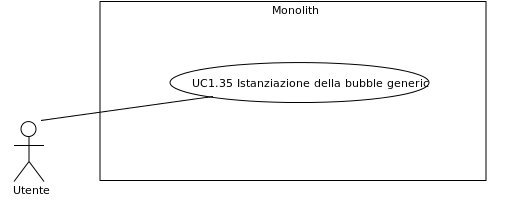
\includegraphics[width=15cm]{../../documenti/AnalisiDeiRequisiti/Diagrammi_img/uc1_35.png}
	\caption{\UCCaption{} Istanziazione della bubble generica}
\end{figure}

\begin{itemize}
	\item \textbf{Attori:}
	\\Utilizzatore del framework.
	\item \textbf{Scopo e descrizione:} 
	\\L'utilizzatore del framework può istanziare il contenitore \glossario{bubble generica}, il quale funge da contenitore dei vari elementi di input, output e di logica specificati all'interno del framework.
	\item \textbf{Flusso principale degli eventi:}
	\\L'utilizzatore del framework chiama il metodo per istanziare la bubble generica e la memoria ad essa associata.
	\item \textbf{Post-condizione:}
	\\È presente la bubble generica, compresa la sua memoria.
\end{itemize}

\UC{Interazione con database MongoDB}{UC2}

\begin{figure}[H]
	\centering
	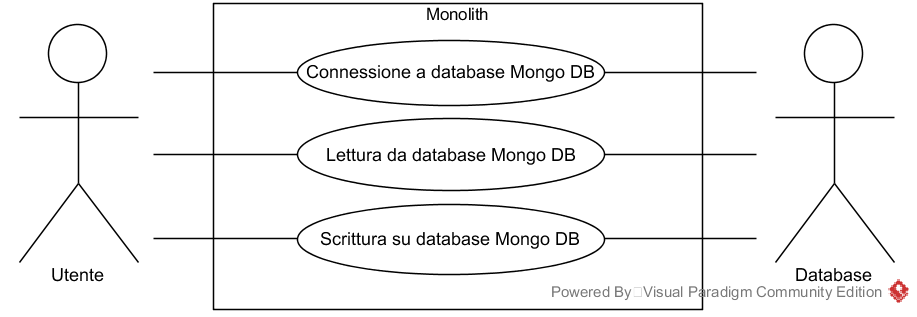
\includegraphics[width=15cm]{../../documenti/AnalisiDeiRequisiti/Diagrammi_img/Database.png}
	\caption{\UCCaption{} Interazione con database MongoDB}
\end{figure}

\begin{itemize}
	\item \textbf{Attori:}
	\\Utilizzatore del framework.
	\item \textbf{Scopo e descrizione:} 
	\\L'utilizzatore del framework interagisce con un database MongoDB esterno.
	\item \textbf{Precondizioni:}
	\begin{itemize}
		\item Avere già istanziato una bubble generica;
		\item Avere l'indirizzo di un database MongoDB con cui si desidera interagire.
	\end{itemize}
	\item \textbf{Flusso principale degli eventi:}
	\\L'utilizzatore del framework interagisce con il database MongoDB di cui possiede l'indirizzo.
	\item \textbf{Post-condizione:}
	\\L'utilizzatore del metodo ha interagito con il database.
\end{itemize}

\pagebreak

\UCF{Connessione a database \glossario{MongoDB}}{UC1.00}

\begin{figure}[H]
	\centering
	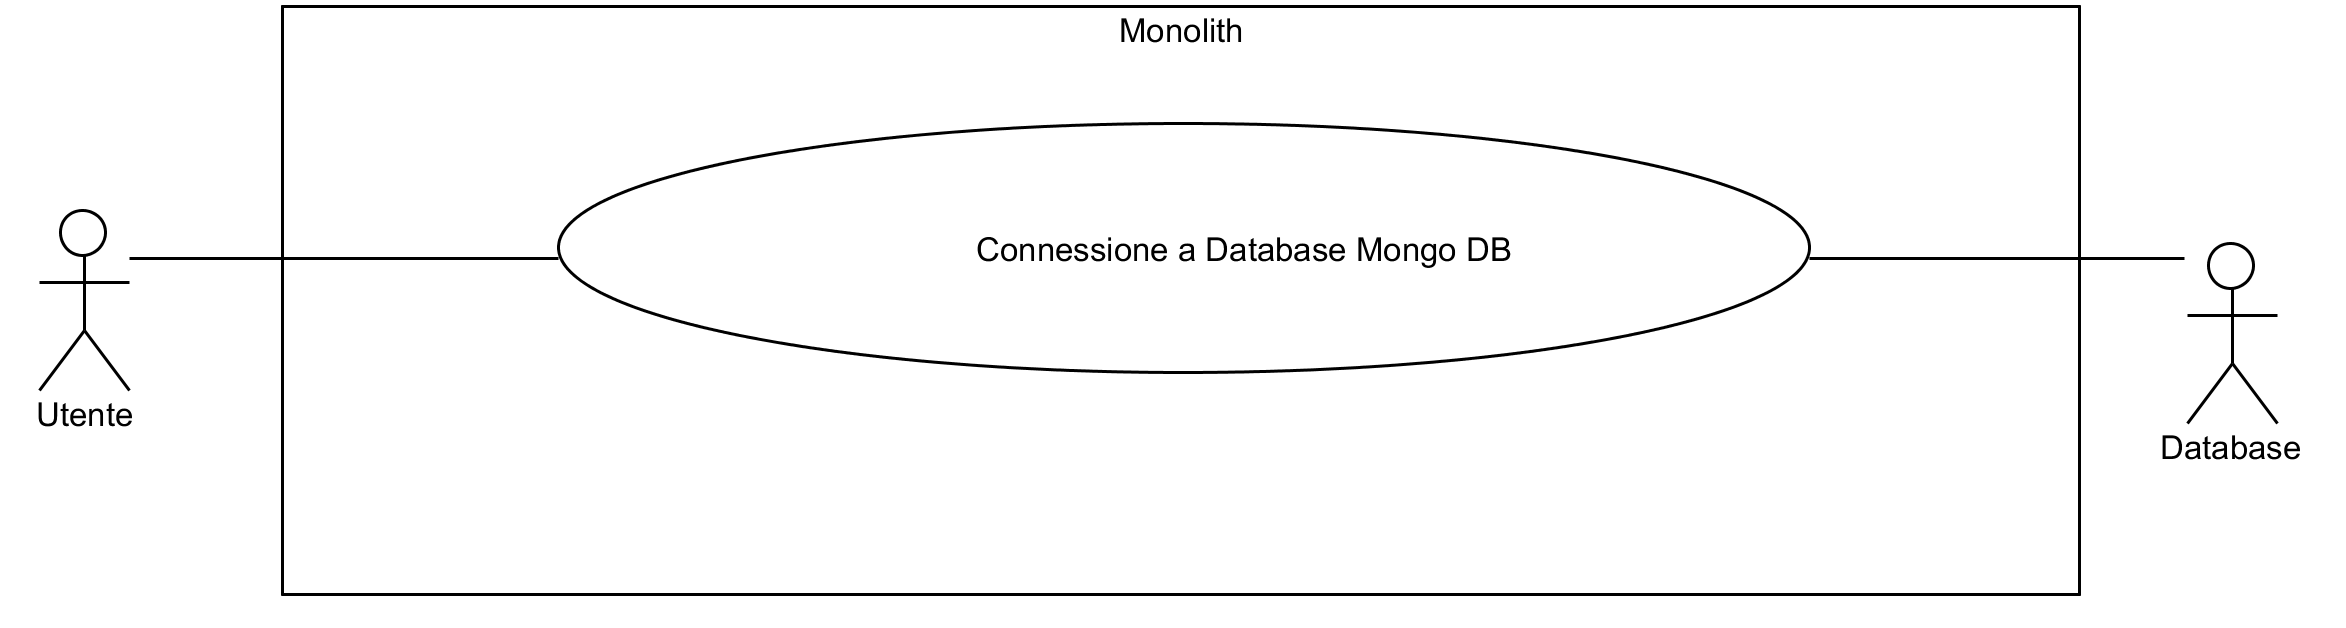
\includegraphics[width=15cm]{../../documenti/AnalisiDeiRequisiti/Diagrammi_img/uc1_00.png}
	\caption{\UCFCaption{} Connessione a database MongoDB}
\end{figure}

\begin{itemize}
\item \textbf{Attori:}
\\Utilizzatore del framework.
\item \textbf{Scopo e descrizione:} 
\\Connettersi ad un database MongoDB esterno all'applicazione.
\item \textbf{Precondizioni:}
	\begin{itemize}
		\item Avere già istanziato una bubble generica;
		\item Avere l'indirizzo del database MongoDB a cui si desidera connettersi.
	\end{itemize}
\item \textbf{Flusso principale degli eventi:}
\\L'utilizzatore passa l'indirizzo del database a cui connettersi al metodo che genera una connessione con il database MongoDB.
\item \textbf{Post-condizione:}
\\La bubble generica da cui è invocato il metodo è connessa al database.
\end{itemize}

\pagebreak

\UCF{Lettura da database MongoDB}{UC1.01}

\begin{figure}[H]
	\centering
	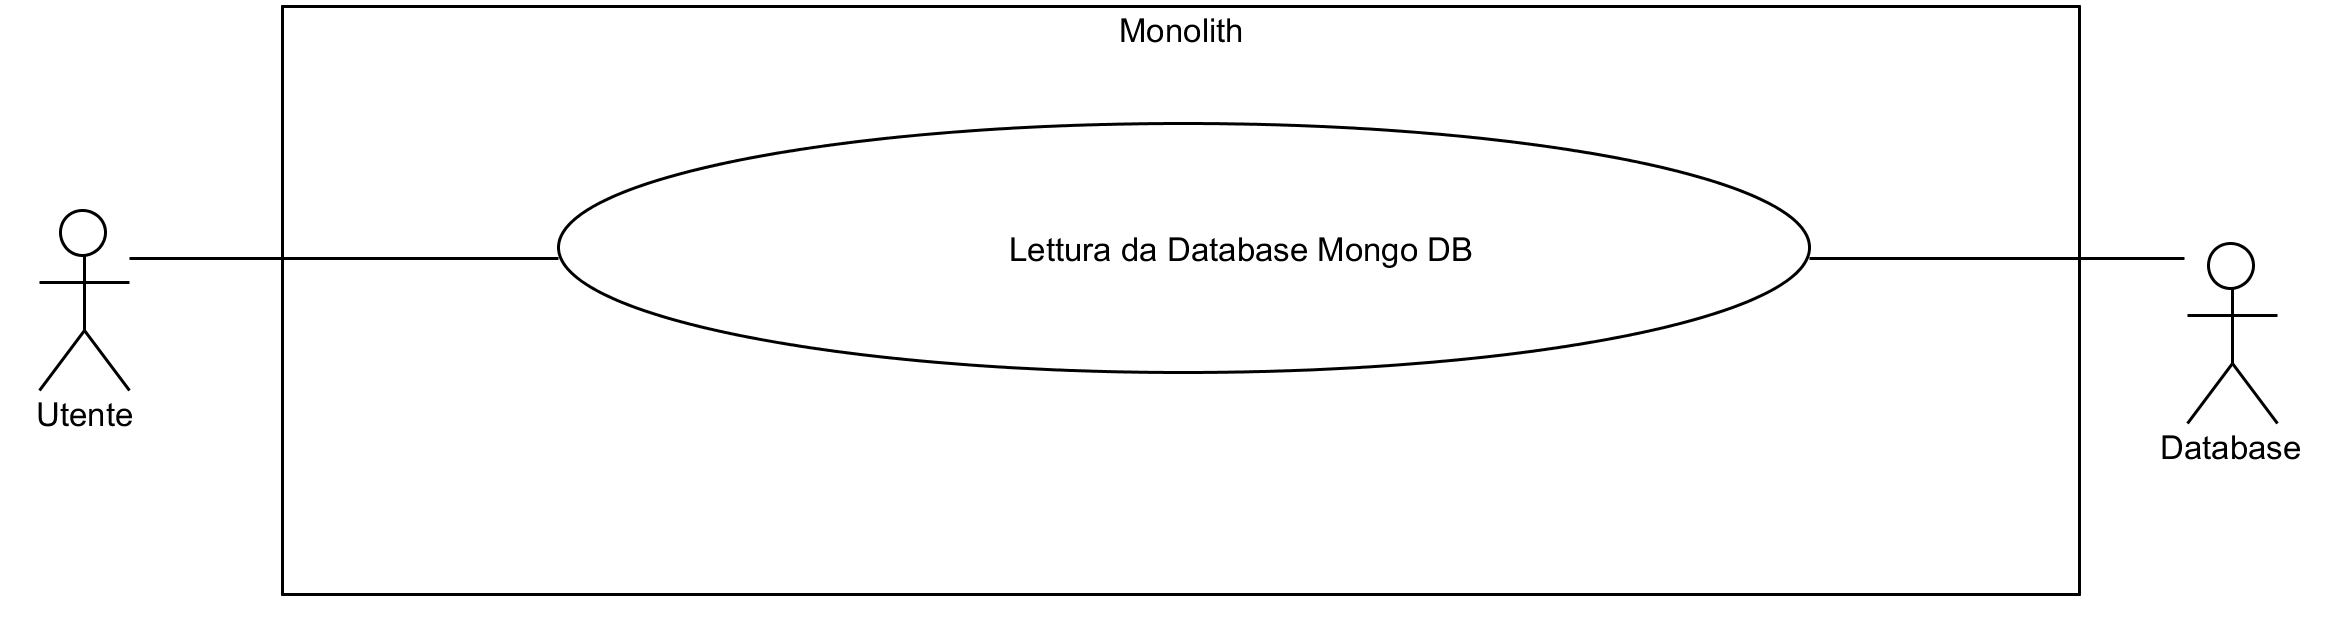
\includegraphics[width=15cm]{../../documenti/AnalisiDeiRequisiti/Diagrammi_img/uc1_01.png}
	\caption{\UCFCaption{} Lettura da database MongoDB}
\end{figure}

\begin{itemize}
	\item \textbf{Attori:}
	\\Utilizzatore del framework.
	\item \textbf{Scopo e descrizione:} 
	\\Prelevare dati dal database connesso alla bubble.
	\item \textbf{Precondizioni:}
	\begin{itemize}
		\item Avere già istanziato una bubble generica;
		\item La bubble è connessa al database MongoDB \ref{UC1.00};
		\item L'utilizzatore deve conoscere il nome della \glossario{collection} da cui prelevare i dati.
	\end{itemize}
	\item \textbf{Flusso principale degli eventi:}
	\\L'utilizzatore chiama il metodo su una bubble, il quale gli ritorna un oggetto \glossario{JSON} letto dal database, eventualmente assegnabile ad un campo della \glossario{bubble memory}.
	\item \textbf{Post-condizione:}
	\\I dati sono prelevati dal database e sono pronti all'uso nella bubble.
\end{itemize}

\pagebreak

\UCF{Scrittura su database MongoDB}{UC1.02}

\begin{figure}[H]
	\centering
	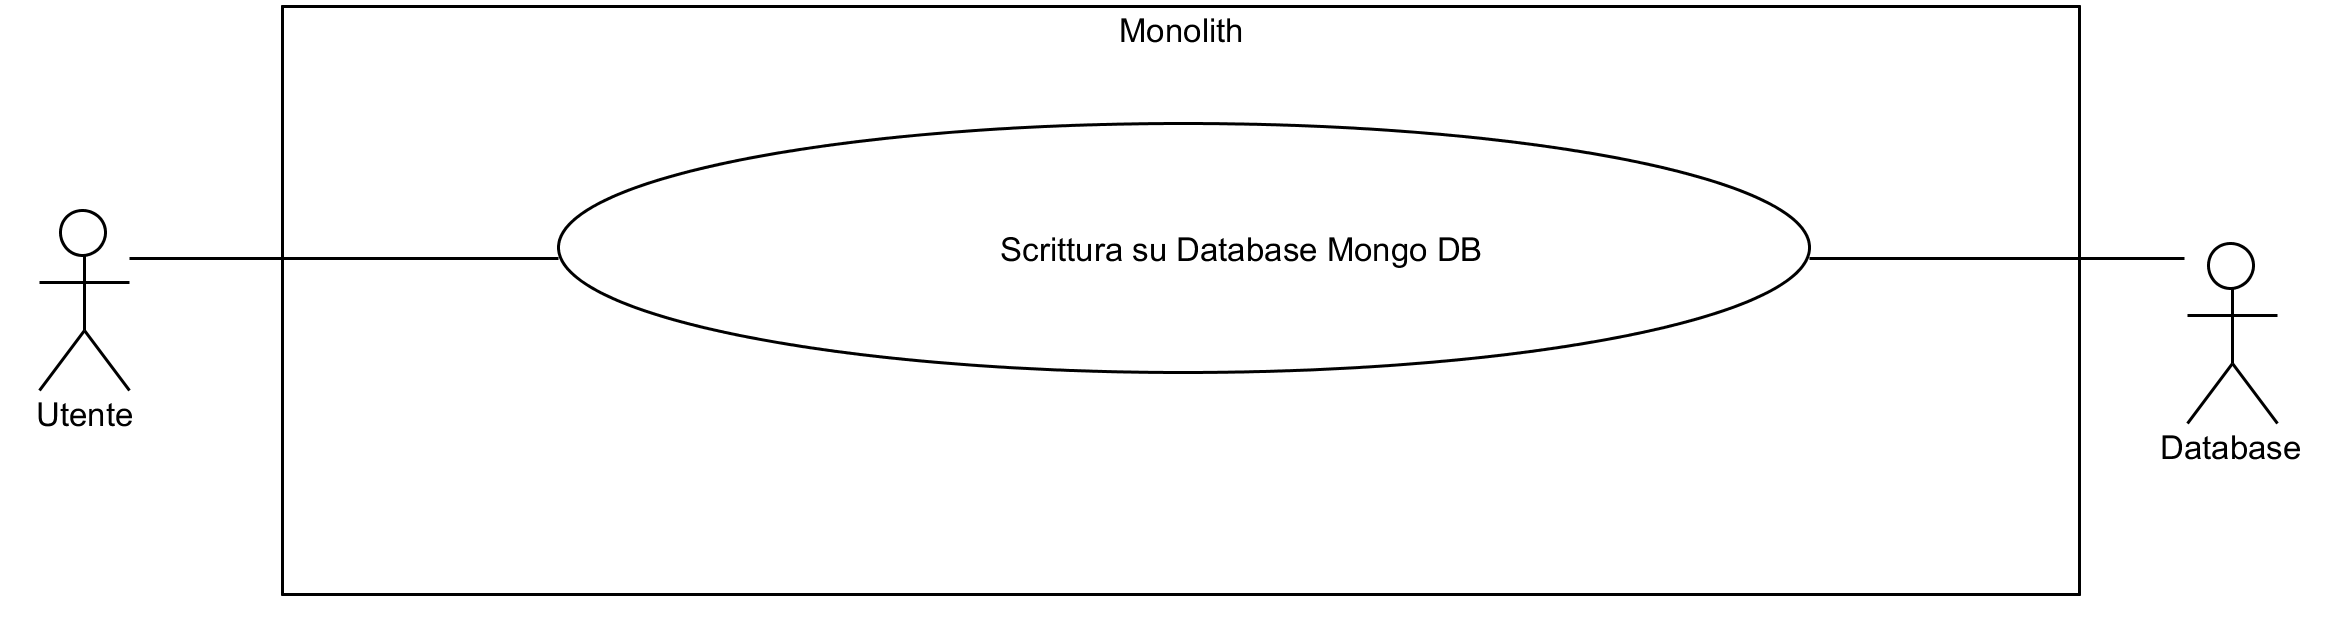
\includegraphics[width=15cm]{../../documenti/AnalisiDeiRequisiti/Diagrammi_img/uc1_02.png}
	\caption{\UCFCaption{} Scrittura su database MongoDB}
\end{figure}

\begin{itemize}
\item \textbf{Attori:}
\\Utilizzatore del framework.
\item \textbf{Scopo e descrizione:} 
\\Scrittura dati nel database connesso alla bubble.
\item \textbf{Precondizioni:}
\begin{itemize}
	\item Avere già istanziato una bubble generica;
	\item La bubble è connessa al database MongoDB \ref{UC1.00};
	\item L'utilizzatore deve conoscere il nome della collection da cui prelevare i dati.
\end{itemize}
\item \textbf{Flusso principale degli eventi:}
\\L'utilizzatore chiama il metodo su una bubble passandogli un oggetto \glossario{JavaScript}, serializzabile in JSON, e il metodo lo salva nel database.
\item \textbf{Post-condizione:}
\\I dati sono scritti nel database collegato.
\end{itemize}

\UC{Effettuare operazioni sugli elementi}{UC1.02}

\begin{figure}[H]
	\centering
	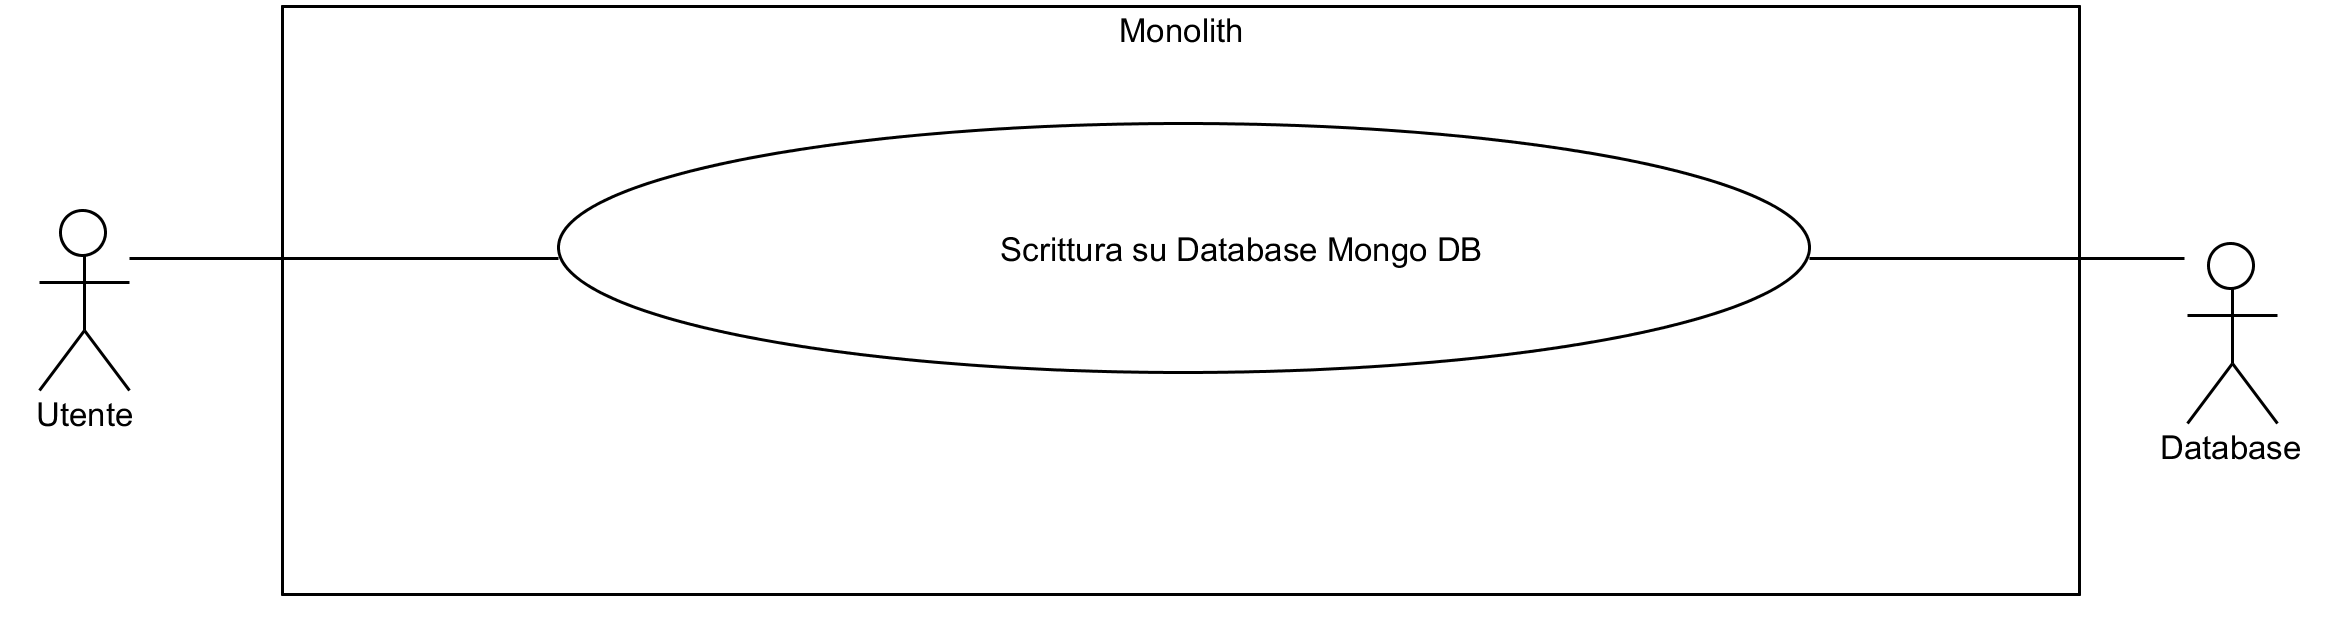
\includegraphics[width=15cm]{../../documenti/AnalisiDeiRequisiti/Diagrammi_img/uc1_02.png}
	\caption{\UCCaption{} Effettuare operazioni sugli elementi}
\end{figure}

\begin{itemize}
	\item \textbf{Attori:}
	\\Utilizzatore del framework.
	\item \textbf{Scopo e descrizione:} 
	\\Effettuare una o più operazioni sugli elementi della bubble.
	\item \textbf{Precondizioni:}
	\begin{itemize}
		\item Avere già istanziato una bubble generica.
	\end{itemize}
	\item \textbf{Flusso principale degli eventi:}
	\\L'utilizzatore effettua delle operazioni sugli elementi della bubble.
	\item \textbf{Post-condizione:}
	\\Sono state apportate delle modifiche agli elementi della bubble.
\end{itemize}

\pagebreak

\UCF{Creazione di un elemento}{UC1.02}

\begin{figure}[H]
	\centering
	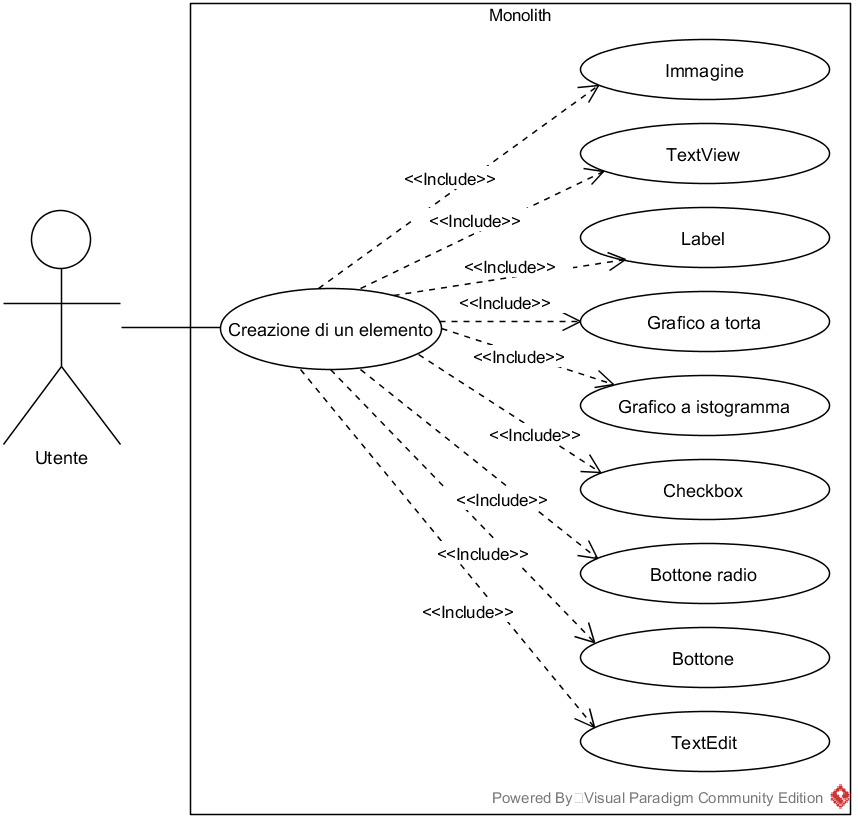
\includegraphics[width=15cm]{../../documenti/AnalisiDeiRequisiti/Diagrammi_img/creazione_elem.png}
	\caption{\UCFCaption{} Creazione di un elemento}
\end{figure}

\begin{itemize}
	\item \textbf{Attori:}
	\\Utilizzatore del framework.
	\item \textbf{Scopo e descrizione:} 
	\\Costruzione di un elemento.
	\item \textbf{Precondizioni:}
	\begin{itemize}
		\item Avere già istanziato una bubble generica;
		\item Disporre di tutte le risorse necessarie a creare l'elemento.
	\end{itemize}
	\item \textbf{Flusso principale degli eventi:}
	\\L'utilizzatore crea l'elemento della tipologia desiderata.
	\item \textbf{Post-condizione:}
	\\È stato creato un elemento.
\end{itemize}

\pagebreak

\UCFF{Immagine}{UC1.25}

\begin{figure}[H]
	\centering
	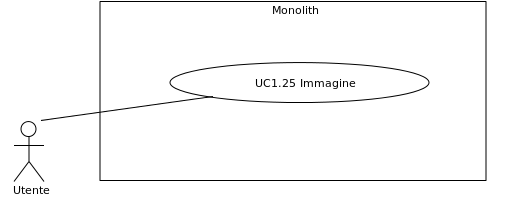
\includegraphics[width=15cm]{../../documenti/AnalisiDeiRequisiti/Diagrammi_img/uc1_25.png}
	\caption{\UCFFCaption{} Immagine}
\end{figure}

\begin{itemize}
	\item \textbf{Attori:}
	\\Utilizzatore del framework.
	\item \textbf{Scopo e descrizione:} 
	\\L'utilizzatore del framework può creare un elemento immagine.
	\item \textbf{Precondizioni:}
	\begin{itemize}
		\item Avere già istanziato una bubble generica;
		\item Avere un'immagine di cui fare la preview.
	\end{itemize}
	\item \textbf{Flusso principale degli eventi:}
	\\L'utilizzatore del framework crea un elemento immagine.
	\item \textbf{Post-condizione:}
	\\È stato creato un elemento immagine.
\end{itemize}

\pagebreak

\UCFF{TextView}{UC1.26}

\begin{figure}[H]
	\centering
	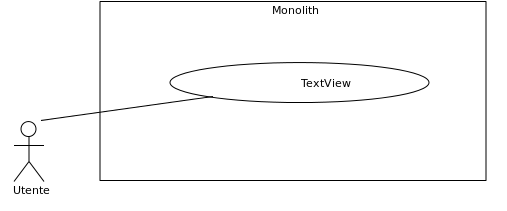
\includegraphics[width=15cm]{../../documenti/AnalisiDeiRequisiti/Diagrammi_img/uc1_26.png}
	\caption{\UCFFCaption{} TextView}
\end{figure}

\begin{itemize}
	\item \textbf{Attori:}
	\\Utilizzatore del framework.
	\item \textbf{Scopo e descrizione:} 
	\\L'utilizzatore del framework può creare un elemento \glossario{TextView}.
	\item \textbf{Precondizioni:}
	\begin{itemize}
		\item Avere già istanziato una bubble generica;
		\item Avere un testo da visualizzare.
	\end{itemize}
	\item \textbf{Flusso principale degli eventi:}
	\\L'utilizzatore del framework crea l'elemento TextView specificando il testo da includere.
	\item \textbf{Post-condizione:}
	\\È stato creato un elemento TextView.
\end{itemize}

\pagebreak

\UCFF{Label}{UC1.27}

\begin{figure}[H]
	\centering
	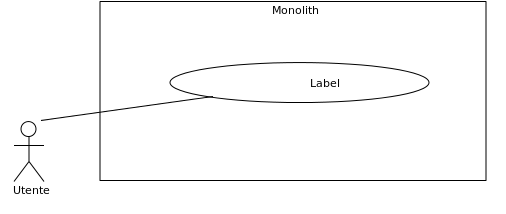
\includegraphics[width=15cm]{../../documenti/AnalisiDeiRequisiti/Diagrammi_img/uc1_27.png}
	\caption{\UCFFCaption{} Label}
\end{figure}

\begin{itemize}
	\item \textbf{Attori:}
	\\Utilizzatore del framework.
	\item \textbf{Scopo e descrizione:} 
	\\L'utilizzatore del framework può creare un elemento \glossario{label}.
	\item \textbf{Precondizioni:}
	\begin{itemize}
		\item Avere già istanziato una bubble generica;
		\item Avere un testo da visualizzare.
	\end{itemize}
	\item \textbf{Flusso principale degli eventi:}
	\\L'utilizzatore del framework crea l'elemento label specificando il testo da includere.
	\item \textbf{Post-condizione:}
	\\È stato creato un elemento label.
\end{itemize}

\pagebreak

\UCFF{Grafico a torta}{UC1.28}

\begin{figure}[H]
	\centering
	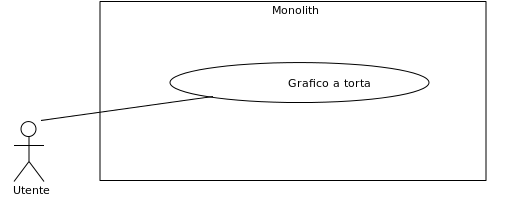
\includegraphics[width=15cm]{../../documenti/AnalisiDeiRequisiti/Diagrammi_img/uc1_28.png}
	\caption{\UCFFCaption{} Grafico a torta}
\end{figure}

\begin{itemize}
	\item \textbf{Attori:}
	\\Utilizzatore del framework.
	\item \textbf{Scopo e descrizione:} 
	\\L'utilizzatore del framework può creare un elemento "grafico a torta".
	\item \textbf{Precondizioni:}
	\begin{itemize}
		\item Avere già istanziato una bubble generica;
		\item Essere in possesso dei dati che si desidera visualizzare nel grafico.
	\end{itemize}
	\item \textbf{Flusso principale degli eventi:}
	\\L'utilizzatore del framework crea l'elemento specificando i dati da rappresentare nel grafico a torta.
	\item \textbf{Post-condizione:}
	\\È stato creato un elemento "grafico a torta".
\end{itemize}

\pagebreak

\UCFF{Grafico a istogramma}{UC1.29}

\begin{figure}[H]
	\centering
	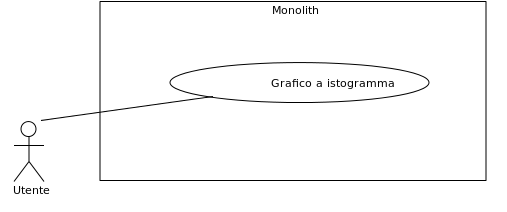
\includegraphics[width=15cm]{../../documenti/AnalisiDeiRequisiti/Diagrammi_img/uc1_29.png}
	\caption{\UCFFCaption{} Grafico a istogramma}
\end{figure}

\begin{itemize}
	\item \textbf{Attori:}
	\\Utilizzatore del framework.
	\item \textbf{Scopo e descrizione:} 
	\\L'utilizzatore del framework può creare un elemento "grafico a istogramma".
	\item \textbf{Precondizioni:}
	\begin{itemize}
		\item Avere già istanziato una bubble generica;
		\item Essere in possesso dei dati che si desidera visualizzare nel grafico.
	\end{itemize}
	\item \textbf{Flusso principale degli eventi:}
	\\L'utilizzatore del framework crea l'elemento specificando i dati da rappresentare nel grafico a istogramma.
	\item \textbf{Post-condizione:}
	\\È stato creato un elemento "grafico a istogramma".
\end{itemize}

\pagebreak

\UCFF{Checkbox}{UC1.30}

\begin{figure}[H]
	\centering
	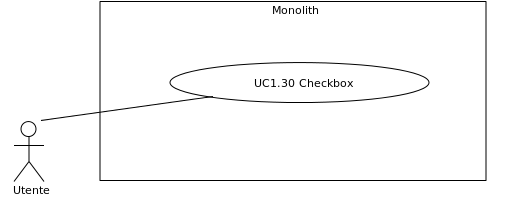
\includegraphics[width=15cm]{../../documenti/AnalisiDeiRequisiti/Diagrammi_img/uc1_30.png}
	\caption{\UCFFCaption{} Checkbox}
\end{figure}

\begin{itemize}
	\item \textbf{Attori:}
	\\Utilizzatore del framework.
	\item \textbf{Scopo e descrizione:} 
	\\L'utilizzatore del framework può creare un elemento \glossario{checkbox}.
	\item \textbf{Precondizioni:}
	\begin{itemize}
		\item Avere già istanziato una bubble generica.
	\end{itemize}
	\item \textbf{Flusso principale degli eventi:}
	\\L'utilizzatore del framework crea l'elemento checkbox.
	\item \textbf{Post-condizione:}
	\\È stato creato l'elemento checkbox.
\end{itemize}

\pagebreak

\UCFF{Bottone Radio}{UC1.31}

\begin{figure}[H]
	\centering
	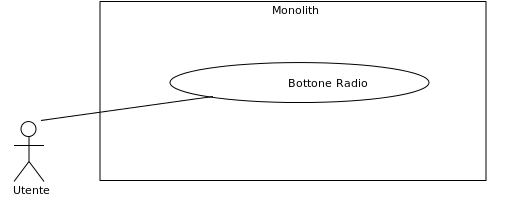
\includegraphics[width=15cm]{../../documenti/AnalisiDeiRequisiti/Diagrammi_img/uc1_31.png}
	\caption{\UCFFCaption{} Bottone Radio}
\end{figure}

\begin{itemize}
	\item \textbf{Attori:}
	\\Utilizzatore del framework.
	\item \textbf{Scopo e descrizione:} 
	\\L'utilizzatore del framework può creare un elemento \glossario{bottone radio}.
	\item \textbf{Precondizioni:}
	\begin{itemize}
		\item Avere già istanziato una bubble generica.
	\end{itemize}
	\item \textbf{Flusso principale degli eventi:}
	\\L'utilizzatore del framework crea un elemento bottone radio.
	\item \textbf{Post-condizione:}
	\\È stato creato l'elemento bottone radio.
\end{itemize}

\pagebreak

\UCFF{Bottone}{UC1.32}

\begin{figure}[H]
	\centering
	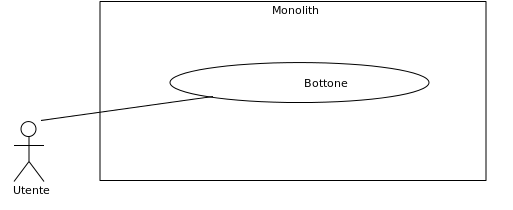
\includegraphics[width=15cm]{../../documenti/AnalisiDeiRequisiti/Diagrammi_img/uc1_32.png}
	\caption{\UCFFCaption{} Bottone}
\end{figure}

\begin{itemize}
	\item \textbf{Attori:}
	\\Utilizzatore del framework.
	\item \textbf{Scopo e descrizione:} 
	\\L'utilizzatore del framework può creare un elemento \glossario{bottone}.
	\item \textbf{Precondizioni:}
	\begin{itemize}
		\item Avere già istanziato una bubble generica;
		\item Avere la funzione da eseguire.
	\end{itemize}
	\item \textbf{Flusso principale degli eventi:}
	\\L'utilizzatore del framework crea l'elemento bottone specificando la funzione da assegnare ad esso.
	\item \textbf{Post-condizione:}
	\\È stato creato un elemento bottone
\end{itemize}

\pagebreak

\UCFF{TextEdit}{UC1.33}

\begin{figure}[H]
	\centering
	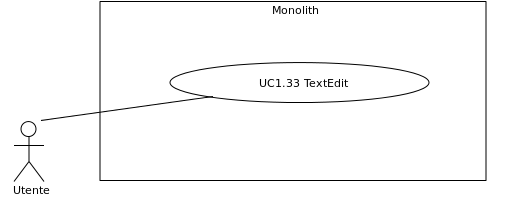
\includegraphics[width=15cm]{../../documenti/AnalisiDeiRequisiti/Diagrammi_img/uc1_33.png}
	\caption{\UCFFCaption{} TextEdit}
\end{figure}

\begin{itemize}
	\item \textbf{Attori:}
	\\Utilizzatore del framework.
	\item \textbf{Scopo e descrizione:} 
	\\L'utilizzatore del framework può creare un input testuale \glossario{TextEdit}.
	\item \textbf{Precondizioni:}
	\begin{itemize}
		\item Avere già istanziato una bubble generica.
	\end{itemize}
	\item \textbf{Flusso principale degli eventi:}
	\\L'utilizzatore del framework crea l'elemento TextEdit.
	\item \textbf{Post-condizione:}
	\\È stato creato l'elemento TextEdit.
\end{itemize}

\pagebreak

\UCF{Aggiunta di un elemento}{UC1.04}

\begin{figure}[H]
	\centering
	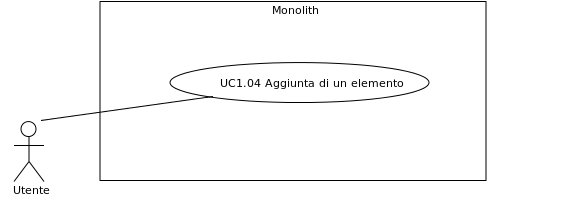
\includegraphics[width=15cm]{../../documenti/AnalisiDeiRequisiti/Diagrammi_img/uc1_04.png}
	\caption{\UCFCaption{} Aggiunta di un elemento}
\end{figure}

\begin{itemize}
	\item \textbf{Attori:}
	\\Utilizzatore del framework.
	\item \textbf{Scopo e descrizione:} 
	\\Inserire nella bubble un elemento.
	\item \textbf{Precondizioni:}
	\begin{itemize}
		\item Avere già istanziato una bubble generica;
		\item Aver istanziato un elemento.
	\end{itemize}
	\item \textbf{Flusso principale degli eventi:}
	\\L'utilizzatore invoca il metodo sulla bubble e il metodo lo aggiunge alla bubble.
	\item \textbf{Post-condizione:}
	\\La bubble avrà al suo interno l'elemento passato al metodo.
\end{itemize}

\pagebreak

\UCC[2]{Rimozione di un elemento presente}{UC1.03.1}

\begin{figure}[H]
	\centering
	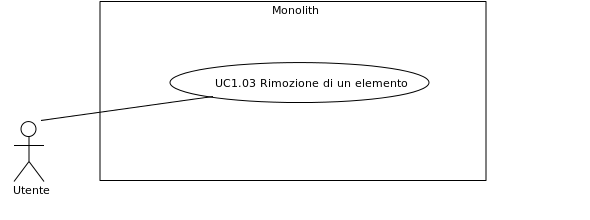
\includegraphics[width=15cm]{../../documenti/AnalisiDeiRequisiti/Diagrammi_img/uc1_03.png}
	\caption{\UCCCaption{} Rimozione di un elemento}
\end{figure}

\begin{itemize}
	\item \textbf{Attori:}
	\\Utilizzatore del framework.
	\item \textbf{Scopo e descrizione:}
	\\Rimuovere dalla bubble un \glossario{elemento}\footnote{Viene considerato elemento del framework un qualsiasi componente grafico (form, immagini, label ad esempio) o funzionale (notifiche, API).} specificato.
	\item \textbf{Precondizioni:}
	\begin{itemize}
		\item Avere già istanziato una bubble generica;
		\item La bubble possiede degli \glossario{elementi}.
	\end{itemize}
	\item \textbf{Flusso principale degli eventi:}
	\\L'utilizzatore chiama il metodo, il quale rimuove l'elemento dalla bubble.
	\item \textbf{Scenari alternativi:}
	\\L'elemento che si vuole eliminare non è presente nella bubble \ref{UC1.03.2}.
	\item \textbf{Post-condizione:}
	\\La bubble non contiene l'elemento indicato da rimuovere.
\end{itemize}

\UCC[2]{Rimozione di un elemento non presente}{UC1.03.2}

\begin{itemize}
	\item \textbf{Attori:}
	\\Utilizzatore del framework.
	\item \textbf{Scopo e descrizione:} 
	\\Rimuovere dalla bubble un elemento specificato.
	\item \textbf{Precondizioni:}
	\begin{itemize}
		\item Avere già istanziato una bubble generica;
		\item La bubble possiede degli elementi.
	\end{itemize}
	\item \textbf{Flusso principale degli eventi:}
	\\L'utilizzatore chiama il metodo, il quale, non trovando l'elemento, restituisce un messaggio di errore.
	\item \textbf{Scenari alternativi:}
	\\L'elemento è presente nella bubble \ref{UC1.03.1}.
	\item \textbf{Post-condizione:}
	\\La bubble non contiene l'elemento indicato da rimuovere e l'utilizzatore è stato avvisato della sua mancanza.
\end{itemize}

\pagebreak
\isfirsttrue

\UCC[2]{Modifica di un elemento presente}{UC1.05.1}

\begin{figure}[H]
	\centering
	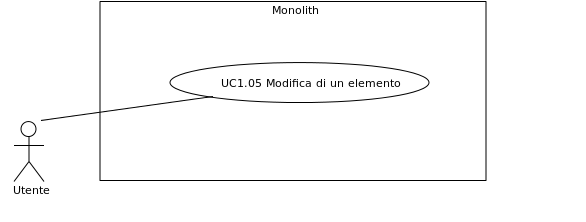
\includegraphics[width=15cm]{../../documenti/AnalisiDeiRequisiti/Diagrammi_img/uc1_05.png}
	\caption{\UCCCaption{} Modifica di un elemento}
\end{figure}

\begin{itemize}
	\item \textbf{Attori:}
	\\Utilizzatore del framework.
	\item \textbf{Scopo e descrizione:} 
	\\Modificare un elemento di una bubble.
	\item \textbf{Precondizioni:}
	\begin{itemize}
		\item Avere già istanziato una bubble generica;
		\item All'interno della bubble sono presenti degli elementi.
	\end{itemize}
	\item \textbf{Flusso principale degli eventi:}
	\\L'utilizzatore invoca il metodo sulla bubble e il metodo modifica l'elemento.
	\item \textbf{Scenari alternativi:}
	\\L'elemento che si vuole modificare non è presente nella bubble \ref{UC1.05.2}.
	\item \textbf{Post-condizione:}
	\\La bubble contiene l'elemento modificato.
\end{itemize}

\UCC[2]{Modifica di un elemento non presente}{UC1.05.2}

\begin{itemize}
	\item \textbf{Attori:}
	\\Utilizzatore del framework.
	\item \textbf{Scopo e descrizione:} 
	\\Modificare un elemento di una bubble.
	\item \textbf{Precondizioni:}
	\begin{itemize}
		\item Avere già istanziato una bubble generica;
		\item All'interno della bubble sono presenti degli elementi.
	\end{itemize}
	\item \textbf{Flusso principale degli eventi:}
	\\L'utilizzatore invoca il metodo sulla bubble e il metodo, non trovando l'elemento da modificare, lancia un messaggio di errore.
	\item \textbf{Scenari alternativi:}
	\\L'elemento è presente nella bubble \ref{UC1.05.1}.
	\item \textbf{Post-condizione:}
	\\L'utilizzatore del metodo è a conoscenza che la modifica è fallita in quanto non era presente l'elemento da modificare.
\end{itemize}

\pagebreak

\UCF{Creazione notifica statica}{UC1.17}

\begin{figure}[H]
	\centering
	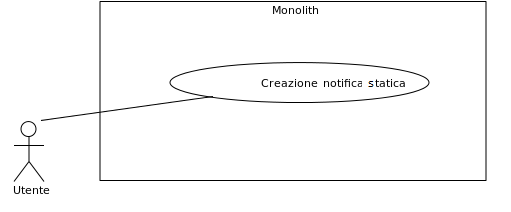
\includegraphics[width=15cm]{../../documenti/AnalisiDeiRequisiti/Diagrammi_img/uc1_17.png}
	\caption{\UCFCaption{} Creazione notifica statica}
\end{figure}

\begin{itemize}
	\item \textbf{Attori:}
	\\Utilizzatore del framework.
	\item \textbf{Scopo e descrizione:} 
	\\L'utilizzatore del framework potrà creare una notifica statica specificandone il testo.
	\item \textbf{Precondizioni:}
	\begin{itemize}
		\item Avere già istanziato una bubble generica;
		\item Essere in possesso del messaggio che si desidera notificare sotto forma di testo.
	\end{itemize}
	\item \textbf{Flusso principale degli eventi:}
	\\L'utilizzatore del framework chiama il metodo specificando il testo da visualizzare nella notifica statica.
	\item \textbf{Post-condizione:}
	\\Sul dispositivo sul quale si sta utilizzando Rocket.Chat sarà notificato il testo specificato nel metodo.
\end{itemize}

\pagebreak

\UCF{Visualizza notifica statica}{UC1.18}

\begin{figure}[H]
	\centering
	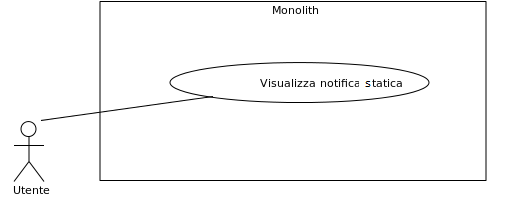
\includegraphics[width=15cm]{../../documenti/AnalisiDeiRequisiti/Diagrammi_img/uc1_18.png}
	\caption{\UCFCaption{} Visualizza notifica statica}
\end{figure}

\begin{itemize}
	\item \textbf{Attori:}
	\\Utilizzatore del framework.
	\item \textbf{Scopo e descrizione:} 
	\\L'utilizzatore del framework può far visualizzare all'utente una notifica statica che visualizzi del testo.
	\item \textbf{Precondizioni:}
	\begin{itemize}
		\item Avere già istanziato una bubble generica;
		\item Aver creato una notifica statica.
	\end{itemize}
	\item \textbf{Flusso principale degli eventi:}
	\\L'utilizzatore del framework fa visualizzare una certa notifica da lui creata.
	\item \textbf{Post-condizione:}
	\\La notifica contiene il valore del testo specificato.
\end{itemize}

\pagebreak

\UCF{Mostra elemento grafico}{UC1.21}

\begin{figure}[H]
	\centering
	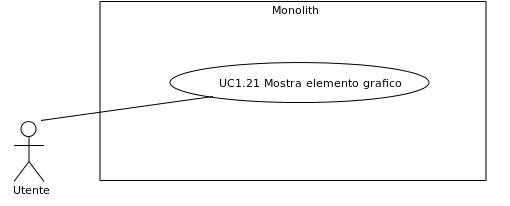
\includegraphics[width=15cm]{../../documenti/AnalisiDeiRequisiti/Diagrammi_img/uc1_21.png}
	\caption{\UCFCaption{} Mostra elemento grafico}
\end{figure}

\begin{itemize}
	\item \textbf{Attori:}
	\\Utilizzatore del framework.
	\item \textbf{Scopo e descrizione:} 
	\\L'utilizzatore del framework potrà mostrare un \glossario{elemento grafico}.\footnote{Esempi di elementi grafici sono: label, immagini, textview.}
	\item \textbf{Precondizioni:}
	\begin{itemize}
		\item Avere già istanziato una bubble generica;
		\item Avere almeno un elemento grafico nella bubble.
	\end{itemize}
	\item \textbf{Flusso principale degli eventi:}
	\\L'utilizzatore del framework chiama il metodo specificando quale elemento grafico della bubble vuole mostrare.
	\item \textbf{Post-condizione:}
	\\L'elemento grafico specificato è visibile.
\end{itemize}

\pagebreak

\UCF{Nascondi elemento grafico}{UC1.22}

\begin{figure}[H]
	\centering
	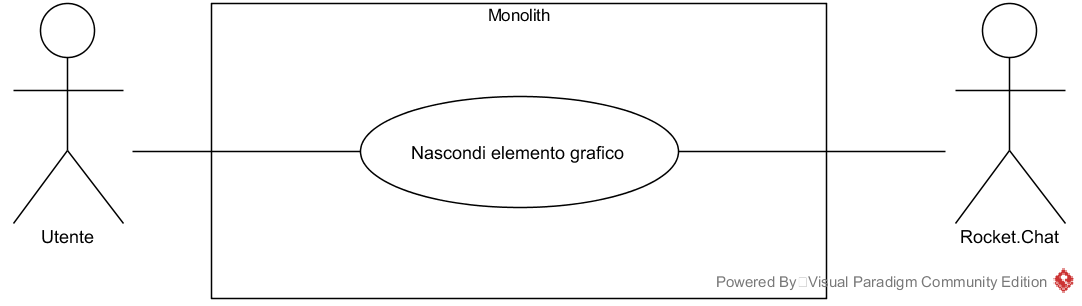
\includegraphics[width=15cm]{../../documenti/AnalisiDeiRequisiti/Diagrammi_img/uc1_22.png}
	\caption{\UCFCaption{} Nascondi elemento grafico}
\end{figure}

\begin{itemize}
	\item \textbf{Attori:}
	\\Utilizzatore del framework.
	\item \textbf{Scopo e descrizione:} 
	\\L'utilizzatore del framework potrà nascondere un elemento grafico.
	\item \textbf{Precondizioni:}
	\begin{itemize}
		\item Avere già istanziato una bubble generica;
		\item Avere almeno un elemento nella bubble.
	\end{itemize}
	\item \textbf{Flusso principale degli eventi:}
	\\L'utilizzatore del framework chiama il metodo specificando quale elemento grafico della bubble vuole nascondere.
	\item \textbf{Post-condizione:}
	\\L'elemento grafico specificato non è più visibile.
\end{itemize}

\pagebreak

\UCF{Imposta posizione elemento grafico}{UC1.23}

\begin{figure}[H]
	\centering
	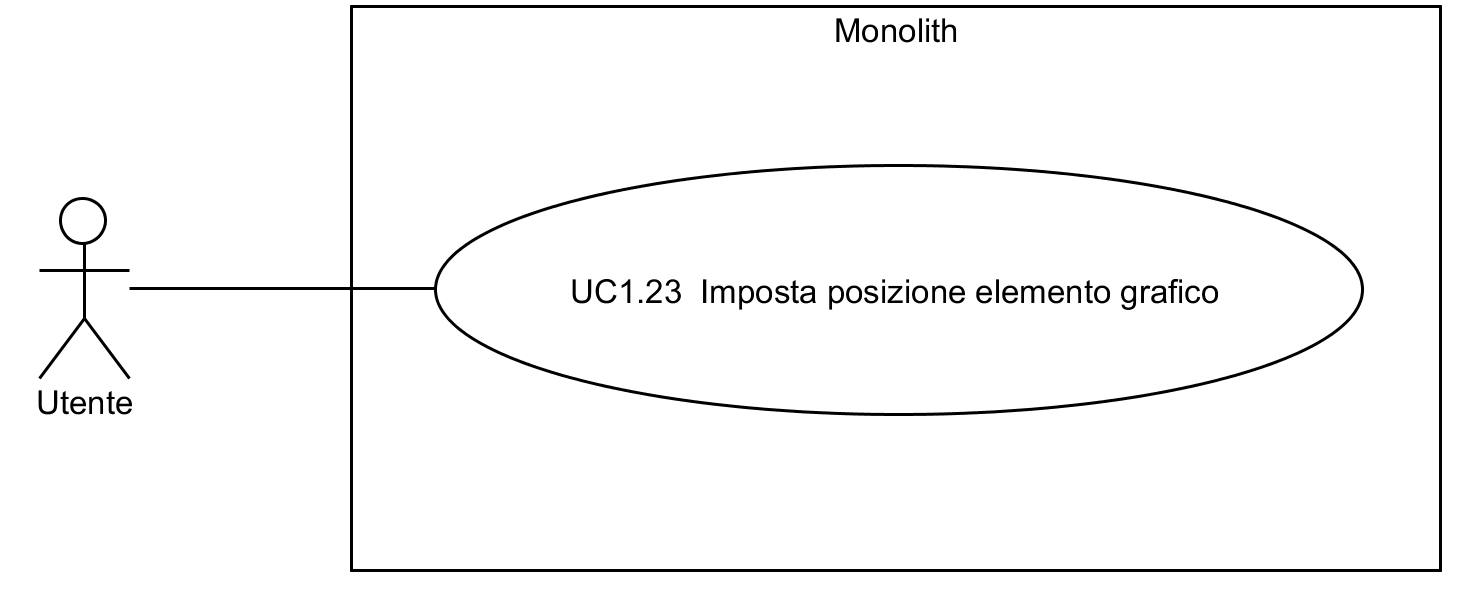
\includegraphics[width=15cm]{../../documenti/AnalisiDeiRequisiti/Diagrammi_img/uc1_23.png}
	\caption{\UCFCaption{} Imposta posizione elemento grafico}
\end{figure}

\begin{itemize}
	\item \textbf{Attori:}
	\\Utilizzatore del framework.
	\item \textbf{Scopo e descrizione:} 
	\\L'utilizzatore del framework può specificare una posizione per un elemento grafico della bubble.
	\item \textbf{Precondizioni:}
	\begin{itemize}
		\item Avere già istanziato una bubble generica;
		\item Avere almeno un componente nella bubble.
	\end{itemize}
	\item \textbf{Flusso principale degli eventi:}
	\\L'utilizzatore del framework chiama il metodo specificando la posizione e l'elemento grafico di cui vuole fissare la posizione.
	\item \textbf{Post-condizione:}
	\\L'elemento grafico specificato si trova nella posizione specificata.
\end{itemize}

\pagebreak
\isfirsttrue

\UCC{Cambiamento di stato della bubble su proprietà esistente}{UC1.06.1}

\begin{figure}[H]
	\centering
	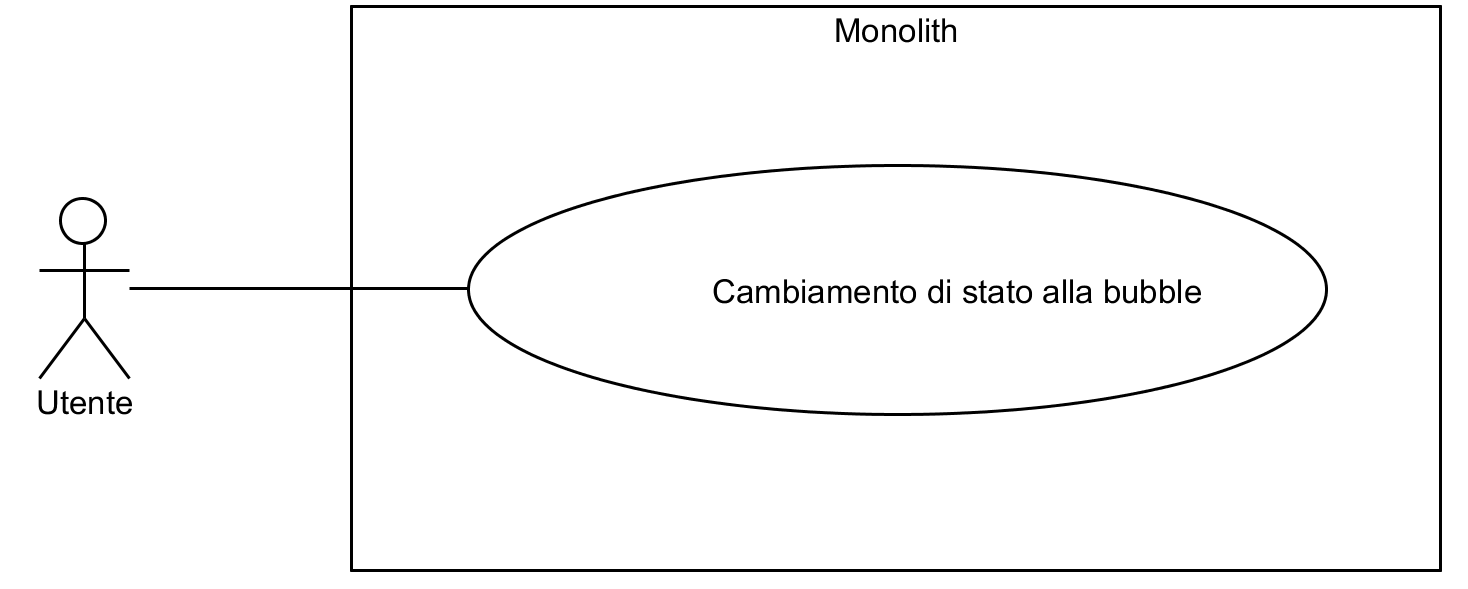
\includegraphics[width=15cm]{../../documenti/AnalisiDeiRequisiti/Diagrammi_img/uc1_06.png}
	\caption{\UCCCaption{} Cambiamento di stato della bubble}
\end{figure}

\begin{itemize}
	\item \textbf{Attori:}
	\\Utilizzatore del framework.
	\item \textbf{Scopo e descrizione:} 
	\\Modificare lo specifico stato della bubble.
	\item \textbf{Precondizioni:}
	\begin{itemize}
		\item Avere già istanziato una bubble generica.
	\end{itemize}
	\item \textbf{Flusso principale degli eventi:}
	\\L'utilizzatore invoca il metodo sulla bubble indicando il nuovo stato e il metodo esegue la modifica.
	\item \textbf{Scenari alternativi:}
	\\L'oggetto che si sta cercando di modificare non ha la proprietà cercata \ref{UC1.06.2}.
	\item \textbf{Post-condizione:}
	\\L'oggetto è stato modificato.
\end{itemize}

\UCC{Cambiamento di stato della bubble su proprietà non esistente}{UC1.06.2}

\begin{itemize}
	\item \textbf{Attori:}
	\\Utilizzatore del framework.
	\item \textbf{Scopo e descrizione:} 
	\\Modificare lo specifico stato della bubble.
	\item \textbf{Precondizioni:}
	\begin{itemize}
		\item Avere già istanziato una bubble generica.
	\end{itemize}
	\item \textbf{Flusso principale degli eventi:}
	\\L'utilizzatore invoca il metodo sulla bubble indicando il nuovo stato e il metodo, non trovando la proprietà cercata, restituisce un messaggio di errore.
	\item \textbf{Scenari alternativi:}
	\\L'oggetto che si sta cercando di modificare ha la proprietà cercata \ref{UC1.06.1}.
	\item \textbf{Post-condizione:}
	\\L'oggetto non è stato modificato.
\end{itemize}

\pagebreak
\isfirsttrue

\UCC{Chiamata API esterne disponibili}{UC1.07.1}

\begin{figure}[H]
	\centering
	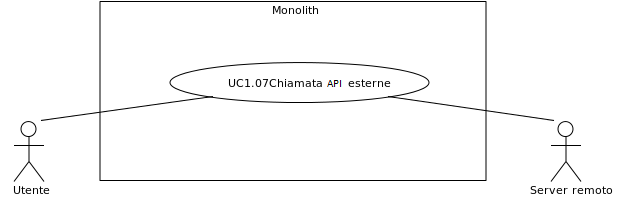
\includegraphics[width=15cm]{../../documenti/AnalisiDeiRequisiti/Diagrammi_img/uc1_07.png}
	\caption{\UCCCaption{} Chiamata API esterne}
\end{figure}

\begin{itemize}
	\item \textbf{Attori:}
	\\Utilizzatore del framework.
	\item \textbf{Scopo e descrizione:} 
	\\Ottenere il risultato dell'interrogazione di un servizio esterno al framework tramite chiamata di \glossario{API}.
	\item \textbf{Precondizioni:}
	\begin{itemize}
		\item Avere già istanziato una bubble generica;
		\item Conoscere l'URL del servizio desiderato.
	\end{itemize}
	\item \textbf{Flusso principale degli eventi:}
	\\Il metodo prende l'indirizzo del servizio e ritorna in formato JSON il risultato della chiamata.
	\item \textbf{Scenari alternativi:}
	\\Il servizio che si sta cercando di contattare non è disponibile \ref{UC1.07.2}.
	\item \textbf{Post-condizione:}
	\\All'interno della logica della bubble è utilizzabile il risultato della consultazione del servizio.
\end{itemize}

\UCC{Chiamata API esterne non disponibili}{UC1.07.2}

\begin{itemize}
	\item \textbf{Attori:}
	\\Utilizzatore del framework.
	\item \textbf{Scopo e descrizione:} 
	\\Ottenere il risultato dell'interrogazione di un servizio esterno al framework tramite chiamata di API.
	\item \textbf{Precondizioni:}
	\begin{itemize}
		\item Avere già istanziato una bubble generica;
		\item Conoscere l'URL del servizio desiderato.
	\end{itemize}
	\item \textbf{Flusso principale degli eventi:}
	\\Il metodo prende l'indirizzo del servizio e, non trovandolo disponibile, ritorna un messaggio di errore.
	\item \textbf{Scenari alternativi:}
	\\Il servizio che si sta cercando di contattare è disponibile \ref{UC1.07.1}.
	\item \textbf{Post-condizione:}
	\\L'utilizzatore del metodo è stato avvisato della non disponibilità del servizio.
\end{itemize}

\UC{Controllo sul JSON}{UC1.12}

\begin{figure}[H]
	\centering
	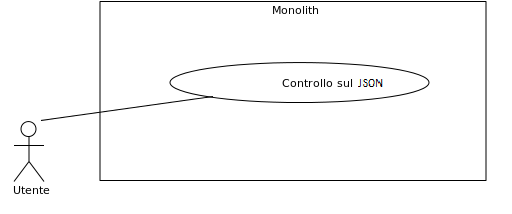
\includegraphics[width=15cm]{../../documenti/AnalisiDeiRequisiti/Diagrammi_img/uc1_12.png}
	\caption{\UCCaption{} Controllo sul JSON}
\end{figure}

\begin{itemize}
	\item \textbf{Attori:}
	\\Utilizzatore del framework.
	\item \textbf{Scopo e descrizione:} 
	\\Verificare che la struttura di un oggetto JSON sia compatibile con lo schema fornito.
	\item \textbf{Precondizioni:}
	\begin{itemize}
		\item Avere già istanziato una bubble generica;
		\item Avere un oggetto JSON da validare;
		\item Avere lo schema attraverso cui validare l'oggetto JSON.
	\end{itemize}
	\item \textbf{Flusso principale degli eventi:}
	\\Alla chiamata del metodo viene specificato il JSON da verificare e lo schema di dati rispetto al quale validare tale oggetto. Il metodo poi si occupa della validazione.
	\item \textbf{Post-condizione:}
	\\È noto se l'oggetto JSON è compatibile con la struttura indicata.
\end{itemize}

\UC{Settare le impostazioni della bubble}{UCimpostazioni}
\begin{figure}[H]
	\centering
	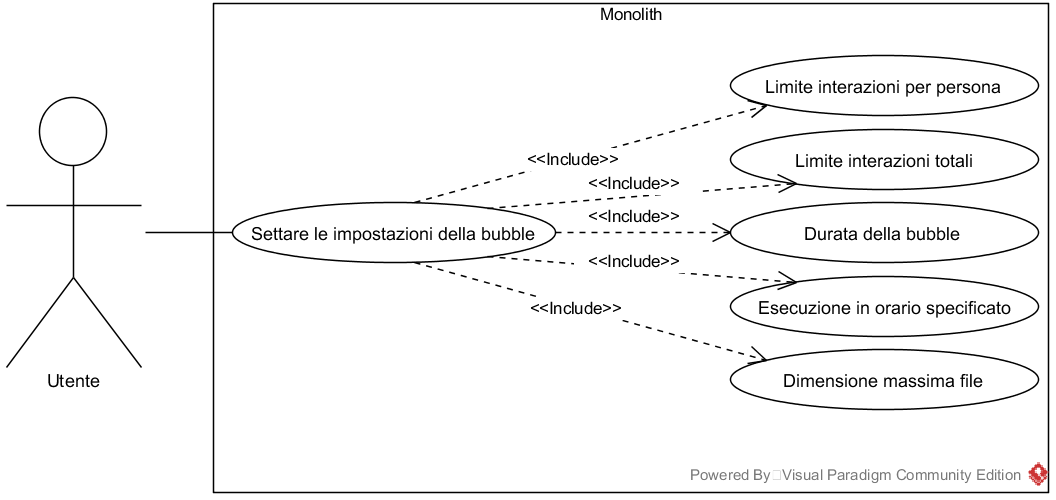
\includegraphics[width=15cm]{../../documenti/AnalisiDeiRequisiti/Diagrammi_img/Impostazioni.png}
	\caption{\UCCaption{} Settare le impostazioni della bubble}
\end{figure}

\begin{itemize}
	\item \textbf{Attori:}
	\\Utilizzatore del framework.
	\item \textbf{Scopo e descrizione:} 
	\\Modificare le impostazioni della bubble per adattarle allo scopo della stessa.
	\item \textbf{Precondizioni:}
	\begin{itemize}
		\item Avere già istanziato una bubble generica;
	\end{itemize}
	\item \textbf{Flusso principale degli eventi:}
	\begin{itemize}
		\item L'utente imposta un limite di interazioni per persona \ref{UC1.08};
		\item L'utente imposta un limite di interazioni totali \ref{UC1.09};
		\item L'utente imposta la durata della bubble \ref{UC1.13};
		\item L'utente specifica l'orario di esecuzione \ref{UC1.16};
		\item L'utente imposta una dimensione massima per i file \ref{}.
	\end{itemize}
	\item \textbf{Post-condizione:}
	\\La bubble è stata configurata con le impostazioni definite.
\end{itemize}

\pagebreak

\UCF{Limite interazioni per persona}{UC1.08}

\begin{figure}[H]
	\centering
	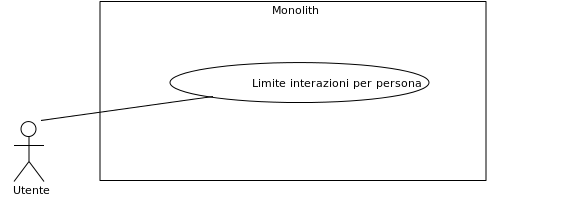
\includegraphics[width=15cm]{../../documenti/AnalisiDeiRequisiti/Diagrammi_img/uc1_08.png}
	\caption{\UCFCaption{} Limite interazioni per persona}
\end{figure}

\begin{itemize}
	\item \textbf{Attori:}
	\\Utilizzatore del framework.
	\item \textbf{Scopo e descrizione:} 
	\\Porre un limite superiore al numero delle interazioni che un utente di Rocket.Chat può avere con una stessa bubble.
	\item \textbf{Precondizioni:}
	\begin{itemize}
		\item Avere già istanziato una bubble generica;
		\item Avere almeno un \glossario{elemento di input} all'interno della bubble.
	\end{itemize}
	\item \textbf{Flusso principale degli eventi:}
	\\Alla chiamata del metodo viene specificato il numero massimo di interazioni possibili per una persona con una singola istanza della bubble.
	\item \textbf{Post-condizione:}
	\\Il singolo utilizzatore della bubble come utente di Rocket.Chat non potrà interagire con la stessa istanza della bubble più volte di quelle specificate.
\end{itemize}

\pagebreak

\UCF{Limite interazioni totali}{UC1.09}

\begin{figure}[H]
	\centering
	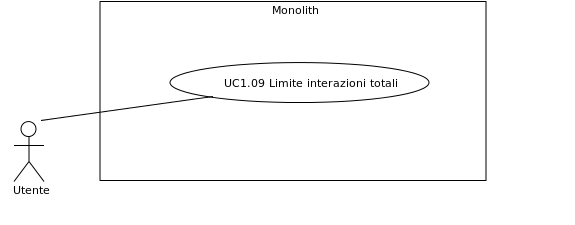
\includegraphics[width=15cm]{../../documenti/AnalisiDeiRequisiti/Diagrammi_img/uc1_09.png}
	\caption{\UCFCaption{} Limite interazioni totali}
\end{figure}

\begin{itemize}
	\item \textbf{Attori:}
	\\Utilizzatore del framework.
	\item \textbf{Scopo e descrizione:} 
	\\Porre un limite superiore al numero delle interazioni che tutti gli utenti possono avere con una stessa istanza della bubble.
	\item \textbf{Precondizioni:}
	\begin{itemize}
		\item Avere già istanziato una bubble generica;
		\item Avere almeno un elemento di input all'interno della bubble.
	\end{itemize}
	\item \textbf{Flusso principale degli eventi:}
	\\Alla chiamata del metodo viene specificato il numero massimo di interazioni possibili per l'istanza della bubble.
	\item \textbf{Post-condizione:}
	\\La singola istanza della bubble ha un numero massimo di interazioni possibili condiviso tra tutti i suoi utenti. 
\end{itemize}

\pagebreak

\UCF{Durata della bubble}{UC1.13}

\begin{figure}[H]
	\centering
	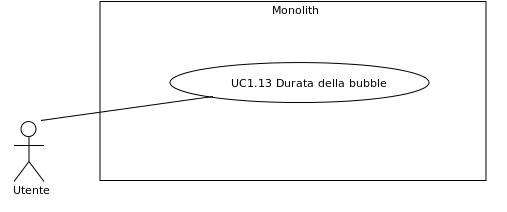
\includegraphics[width=15cm]{../../documenti/AnalisiDeiRequisiti/Diagrammi_img/uc1_13.png}
	\caption{\UCFCaption{} Durata della bubble}
\end{figure}

\begin{itemize}
	\item \textbf{Attori:}
	\\Utilizzatore del framework.
	\item \textbf{Scopo e descrizione:} 
	\\Dare la possibilità all'utilizzatore del framework di impostare un limite temporale entro il quale la bubble smetterà di essere attiva.
	\item \textbf{Precondizioni:}
	\begin{itemize}
		\item Avere già istanziato una bubble generica.
	\end{itemize}
	\item \textbf{Flusso principale degli eventi:}
	\\Alla chiamata del metodo viene specificato il tempo per il quale la bubble sarà attiva.
	\item \textbf{Post-condizione:}
	\\Al termine del periodo di tempo specificato dal metodo verrà invocata la sua terminazione secondo quanto specificato nel caso d'uso \ref{UC1.19} termina bubble.
\end{itemize}

\pagebreak

\UCF{Esecuzione in orario specificato}{UC1.16}

\begin{figure}[H]
	\centering
	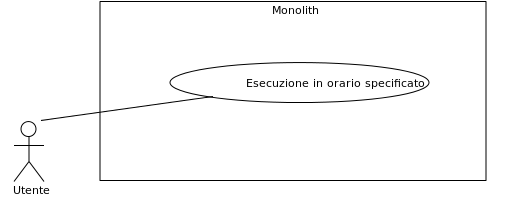
\includegraphics[width=15cm]{../../documenti/AnalisiDeiRequisiti/Diagrammi_img/uc1_16.png}
	\caption{\UCFCaption{} Esecuzione in orario specificato}
\end{figure}

\begin{itemize}
	\item \textbf{Attori:}
	\\Utilizzatore del framework.
	\item \textbf{Scopo e descrizione:} 
	\\L'utilizzatore del framework può fornire un orario per l'esecuzione della funzionalità della bubble.
	\item \textbf{Precondizioni:}
	\begin{itemize}
		\item Avere già istanziato una bubble generica;
		\item Avere la funzione di callback che si desidera eseguire all'orario specificato.
	\end{itemize}
	\item \textbf{Flusso principale degli eventi:}
	\\Alla chiamata del metodo viene specificato l'orario di esecuzione della specifica funzionalità della bubble.
	\item \textbf{Post-condizione:}
	\\Nell'orario stabilito viene eseguita la funzionalità della bubble.
\end{itemize}

\pagebreak

\UCF{Dimensione massima del file}{UC1.11}

\begin{figure}[H]
	\centering
	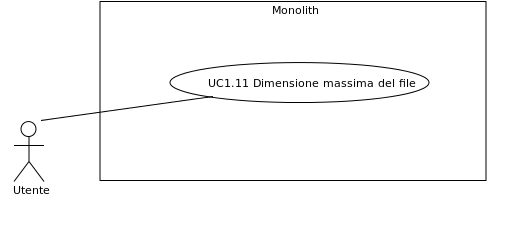
\includegraphics[width=15cm]{../../documenti/AnalisiDeiRequisiti/Diagrammi_img/uc1_11.png}
	\caption{\UCFCaption{} Dimensione massima del file}
\end{figure}

\begin{itemize}
	\item \textbf{Attori:}
	\\Utilizzatore del framework.
	\item \textbf{Scopo e descrizione:} 
	\\Verificare che la dimensione dei file caricati in input sia minore o uguale a quella specificata.
	\item \textbf{Precondizioni:}
	\begin{itemize}
		\item Avere già istanziato una bubble generica;
		\item Avere almeno un elemento di input all'interno della bubble.
	\end{itemize}
	\item \textbf{Flusso principale degli eventi:}
	\\Alla chiamata del metodo viene specificata la dimensione massima accettata per i file di input.
	\item \textbf{Post-condizione:}
	\\È stata impostata una dimensione massima per i file allegabili.
\end{itemize}

\UC{Match con espressione regolare}{UC1.10}

\begin{figure}[H]
	\centering
	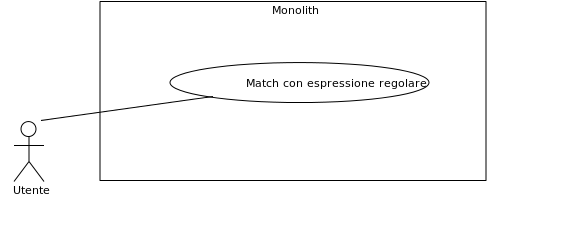
\includegraphics[width=15cm]{../../documenti/AnalisiDeiRequisiti/Diagrammi_img/uc1_10.png}
	\caption{\UCCaption{} Match con espressione regolare}
\end{figure}

\begin{itemize}
	\item \textbf{Attori:}
	\\Utilizzatore del framework.
	\item \textbf{Scopo e descrizione:} 
	\\Verificare che l'input testuale di una bubble sia compatibile con un'espressione regolare data.
	\item \textbf{Precondizioni:}
	\begin{itemize}
		\item Avere già istanziato una bubble generica;
		\item Avere almeno un elemento di input all'interno della bubble.
	\end{itemize}
	\item \textbf{Flusso principale degli eventi:}
	\\Alla chiamata del metodo viene specificato l'elemento da verificare e l'espressione regolare in base a cui controllarlo.
	\item \textbf{Post-condizione:}
	\\È noto se l'input della bubble è corretto secondo l'espressione regolare.
\end{itemize}

\UC{Lista utenti partecipanti}{UC1.14}

\begin{figure}[H]
	\centering
	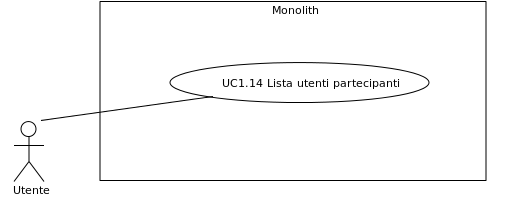
\includegraphics[width=15cm]{../../documenti/AnalisiDeiRequisiti/Diagrammi_img/uc1_14.png}
	\caption{\UCCaption{} Lista utenti partecipanti}
\end{figure}

\begin{itemize}
	\item \textbf{Attori:}
	\\Utilizzatore del framework.
	\item \textbf{Scopo e descrizione:} 
	\\Possibilità di visualizzare gli utilizzatori correnti della bubble.
	\item \textbf{Precondizioni:}
	\begin{itemize}
		\item Avere già istanziato una bubble generica.
	\end{itemize}
	\item \textbf{Flusso principale degli eventi:}
	\\Alla chiamata del metodo viene specificato l'elenco degli utilizzatori correnti della bubble.
	\item \textbf{Post-condizione:}
	\\Viene restituita una lista di utilizzatori della bubble.
\end{itemize}

\pagebreak

\UCC{Storico interazioni con la bubble per utente presente}{UC1.15.1}

\begin{figure}[H]
	\centering
	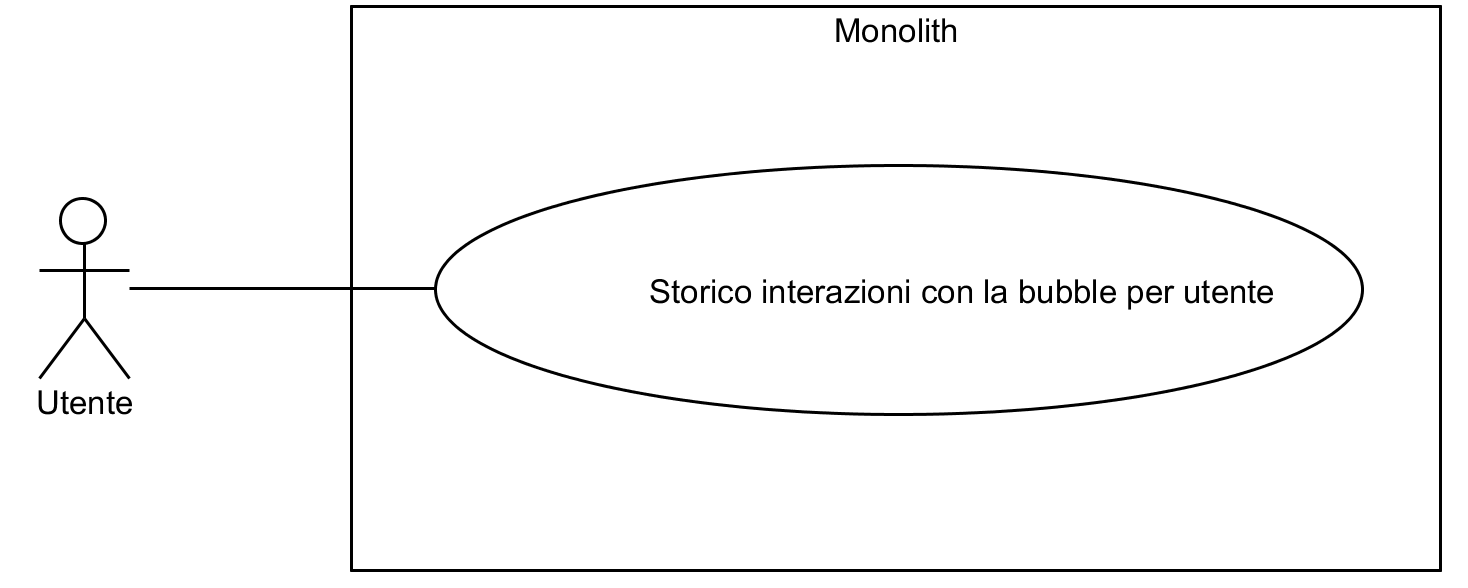
\includegraphics[width=15cm]{../../documenti/AnalisiDeiRequisiti/Diagrammi_img/uc1_15.png}
	\caption{\UCCCaption{} Storico interazioni con la bubble per utente}
\end{figure}

\begin{itemize}
	\item \textbf{Attori:}
	\\Utilizzatore del framework.
	\item \textbf{Scopo e descrizione:} 
	\\Dare la possibilità all'utilizzatore del framework di consultare lo storico delle interazioni che un singolo utente ha avuto con la bubble.
	\item \textbf{Precondizioni:}
	\begin{itemize}
		\item Avere già istanziato una bubble generica;
		\item Avere elementi di input all'interno della bubble.
	\end{itemize}
	\item \textbf{Flusso principale degli eventi:}
	\\Alla chiamata del metodo viene specificato l'utente di cui si è interessati a conoscere lo storico delle interazioni.
	\item \textbf{Scenari alternativi:}
	\\Non è presente l'utente specificato all'interno della conversazione \ref{UC1.15.2}.
	\item \textbf{Post-condizione:}
	\\L'informazione relativa allo storico delle interazioni di un singolo utente con la bubble è noto all'interno della bubble stessa.
\end{itemize}

\UCC{Storico interazioni con la bubble per utente non presente}{UC1.15.2}

\begin{itemize}
	\item \textbf{Attori:}
	\\Utilizzatore del framework.
	\item \textbf{Scopo e descrizione:} 
	\\Dare la possibilità all'utilizzatore del framework di consultare lo storico delle interazioni che un singolo utente ha avuto con la bubble.
	\item \textbf{Precondizioni:}
	\begin{itemize}
		\item Avere già istanziato una bubble generica;
		\item Avere elementi di input all'interno della bubble.
	\end{itemize}
	\item \textbf{Flusso principale degli eventi:}
	\\Alla chiamata del metodo viene specificato l'utente di cui si è interessati a conoscere lo storico delle interazioni e il metodo, non trovando l'utente, restituisce un messaggio di errore.
	\item \textbf{Scenari alternativi:}
	\\È presente l'utente specificato all'interno della conversazione \ref{UC1.15.1}.
	\item \textbf{Post-condizione:}
	\\L'utilizzatore del metodo ha ricevuto un messaggio di errore che lo avvisa dell'assenza all'interno della conversazione dell'utente di cui aveva richiesto lo storico.
\end{itemize}

\pagebreak

\UCC{Converti in PDF}{UC1.20.1}

\begin{figure}[H]
	\centering
	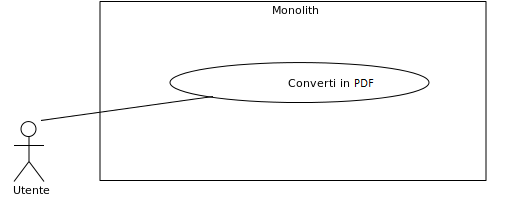
\includegraphics[width=15cm]{../../documenti/AnalisiDeiRequisiti/Diagrammi_img/uc1_20.png}
	\caption{\UCCCaption{} Converti in PDF}
\end{figure}

\begin{itemize}
	\item \textbf{Attori:}
	\\Utilizzatore del framework.
	\item \textbf{Scopo e descrizione:} 
	\\L'utilizzatore del framework potrà convertire il testo specificato in un \glossario{PDF}.
	\item \textbf{Precondizioni:}
	\begin{itemize}
		\item Avere già istanziato una bubble generica;
		\item Possedere il testo da convertire in formato PDF;
		\item Conoscere il percorso in cui si desidera che il file sia salvato.
	\end{itemize}
	\item \textbf{Flusso principale degli eventi:}
	\\L'utilizzatore del framework chiama il metodo specificando il testo da convertire in PDF e il percorso in cui si desidera salvare il file.
	\item \textbf{Scenari alternativi:}
	\\Il salvataggio del file PDF non ha successo \ref{UC1.20.2}.
	\item \textbf{Post-condizione:}
	\\Un file PDF è stato creato nella posizione corretta e contiene il testo specificato.
\end{itemize}

\UCC{Conversione in PDF fallita}{UC1.20.2}

\begin{itemize}
	\item \textbf{Attori:}
	\\Utilizzatore del framework.
	\item \textbf{Scopo e descrizione:} 
	\\L'utilizzatore del framework potrà convertire il testo specificato in un PDF.
	\item \textbf{Precondizioni:}
	\begin{itemize}
		\item Avere già istanziato una bubble generica;
		\item Possedere il testo da convertire in formato PDF;
		\item Conoscere il percorso in cui si desidera che il file sia salvato.
	\end{itemize}
	\item \textbf{Flusso principale degli eventi:}
	\\L'utilizzatore del framework chiama il metodo specificando il testo da convertire in PDF e il percorso in cui si desidera salvare il file, ma il salvataggio non avviene e l'utilizzatore del framework visualizza un messaggio d'errore.
	\item \textbf{Scenari alternativi:}
	\\Il salvataggio del file PDF ha successo \ref{UC1.20.2}.
	\item \textbf{Post-condizione:}
	\\L'utilizzatore del metodo ha ricevuto un messaggio di errore che lo avvisa che il file PDF non è stato salvato.
\end{itemize}

\pagebreak
\isfirsttrue

\UCC{File output}{UC1.24.1}

\begin{figure}[H]
	\centering
	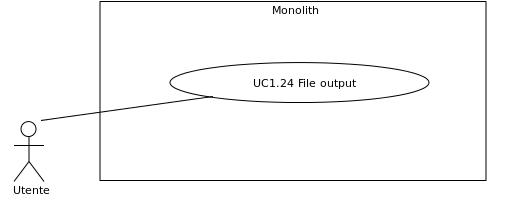
\includegraphics[width=15cm]{../../documenti/AnalisiDeiRequisiti/Diagrammi_img/uc1_24.png}
	\caption{\UCCCaption{} File output}
\end{figure}

\begin{itemize}
	\item \textbf{Attori:}
	\\Utilizzatore del framework.
	\item \textbf{Scopo e descrizione:} 
	\\L'utilizzatore del framework può salvare l'output della bubble in un file.
	\item \textbf{Precondizioni:}
	\begin{itemize}
		\item Avere già istanziato una bubble generica;
		\item Avere almeno un elemento nella bubble.
	\end{itemize}
	\item \textbf{Flusso principale degli eventi:}
	\\L'utilizzatore del framework chiama il metodo che specifica che l'output della bubble sia un file e le informazioni da salvare in esso.
	\item \textbf{Scenari alternativi:}
	\\Il salvataggio del file non ha successo, in tale caso verrà notificata la condizione anomala con un messaggio d'errore \ref{UC1.24.2}.
	\item \textbf{Post-condizione:}
	\\Verrà generato un file contenente l'informazione desiderata.
\end{itemize}

\UCC{Errore File output}{UC1.24.2}

\begin{itemize}
	\item \textbf{Attori:}
	\\Utilizzatore del framework.
	\item \textbf{Scopo e descrizione:} 
	\\L'utilizzatore del framework può salvare l'output della bubble in un file, il salvataggio non va a buon fine e viene generato un messaggio d'errore.
	\item \textbf{Precondizioni:}
	\begin{itemize}
		\item Avere già istanziato una bubble generica;
		\item Avere delle informazioni da esportare.
	\end{itemize}
	\item \textbf{Flusso principale degli eventi:}
	\\L'utilizzatore del framework chiama il metodo che specifica che l'output della bubble sia un file e le informazioni da salvare in esso, il salvataggio non va a buon fine e viene generato un messaggio d'errore.
	\item \textbf{Scenari alternativi:}
	\\Il salvataggio del file ha successo \ref{UC1.24.1}.
	\item \textbf{Post-condizione:}
	\\Viene generato un messaggio d'errore.
\end{itemize}

\UC{File input}{UC1.34}

\begin{figure}[H]
	\centering
	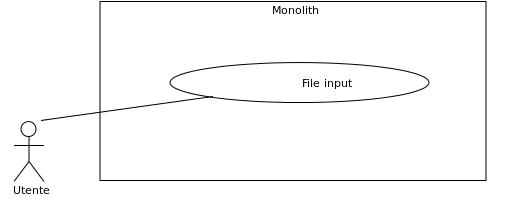
\includegraphics[width=15cm]{../../documenti/AnalisiDeiRequisiti/Diagrammi_img/uc1_34.png}
	\caption{\UCCaption{} File input}
\end{figure}

\begin{itemize}
	\item \textbf{Attori:}
	\\Utilizzatore del framework.
	\item \textbf{Scopo e descrizione:} 
	\\L'utilizzatore del framework può richiedere l'input di un file.
	\item \textbf{Precondizioni:}
	\begin{itemize}
		\item Avere già istanziato una bubble generica.
	\end{itemize}
	\item \textbf{Flusso principale degli eventi:}
	\\L'utilizzatore del framework chiama il metodo che restituisce il file in input.
	\item \textbf{Post-condizione:}
	\\Il file è stato caricato e passato alla bubble.
\end{itemize}

\UC{Mostra bubble generica}{UC1.36}

\begin{figure}[H]
	\centering
	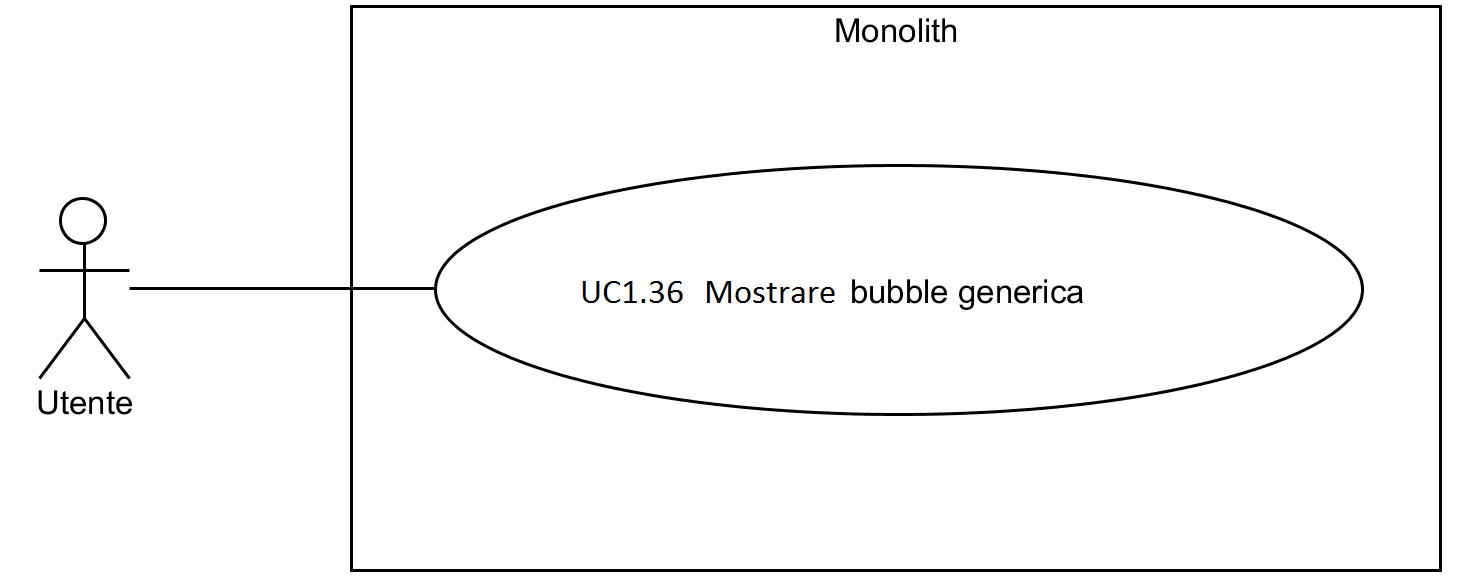
\includegraphics[width=15cm]{../../documenti/AnalisiDeiRequisiti/Diagrammi_img/uc1_36.png}
	\caption{UC1.36 Mostrare bubble generica}
\end{figure}

\begin{itemize}
	\item \textbf{Attori:}
	\\Utilizzatore del framework.
	\item \textbf{Scopo e descrizione:} 
	\\L'utilizzatore del framework, utilizzando questo metodo, rende la bubble visibile all'interno della chat.
	\item \textbf{Precondizioni:}
	\begin{itemize}
		\item Avere già istanziato una bubble generica.
	\end{itemize}
	\item \textbf{Flusso principale degli eventi:}
	\\L'utilizzatore del framework chiama il metodo.
	\item \textbf{Post-condizione:}
	\\La bubble specificata viene mostrata all'interno della chat.
\end{itemize}

\UC{Termina bubble}{UC1.19}

\begin{figure}[H]
	\centering
	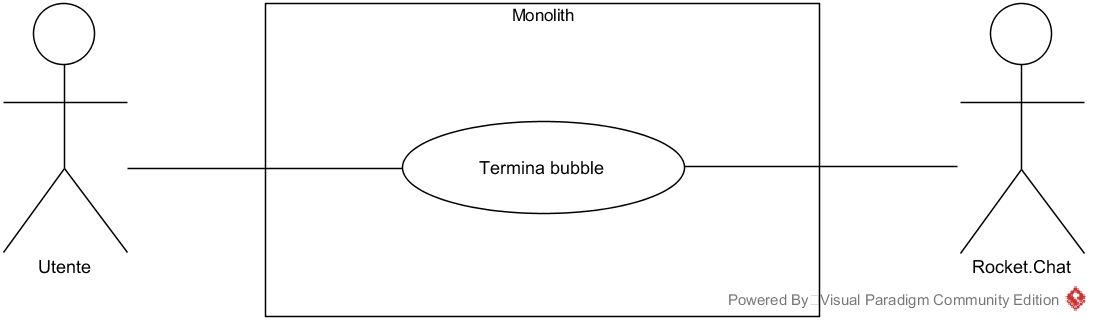
\includegraphics[width=15cm]{../../documenti/AnalisiDeiRequisiti/Diagrammi_img/uc1_19.png}
	\caption{\UCCaption{} Termina bubble}
\end{figure}

\begin{itemize}
	\item \textbf{Attori:}
	\\Utilizzatore del framework.
	\item \textbf{Scopo e descrizione:} 
	\\L'utilizzatore del framework potrà terminare la bubble.
	\item \textbf{Precondizioni:}
	\begin{itemize}
		\item Avere già istanziato una bubble generica.
	\end{itemize}
	\item \textbf{Flusso principale degli eventi:}
	\\L'utilizzatore del framework chiama il metodo.
	\item \textbf{Post-condizione:}
	\\La bubble è stata terminata e quindi non sarà più possibile interagire con la stessa. L'interfaccia verrà aggiornata, disabilitando la possibilità di dare input e avere output dinamico ma mantenendo un'istantanea del suo ultimo stato.
\end{itemize}

\subsection{To-do list}

\UC{Creare una lista}{UC2.1}

\begin{figure}[H]
	\centering
	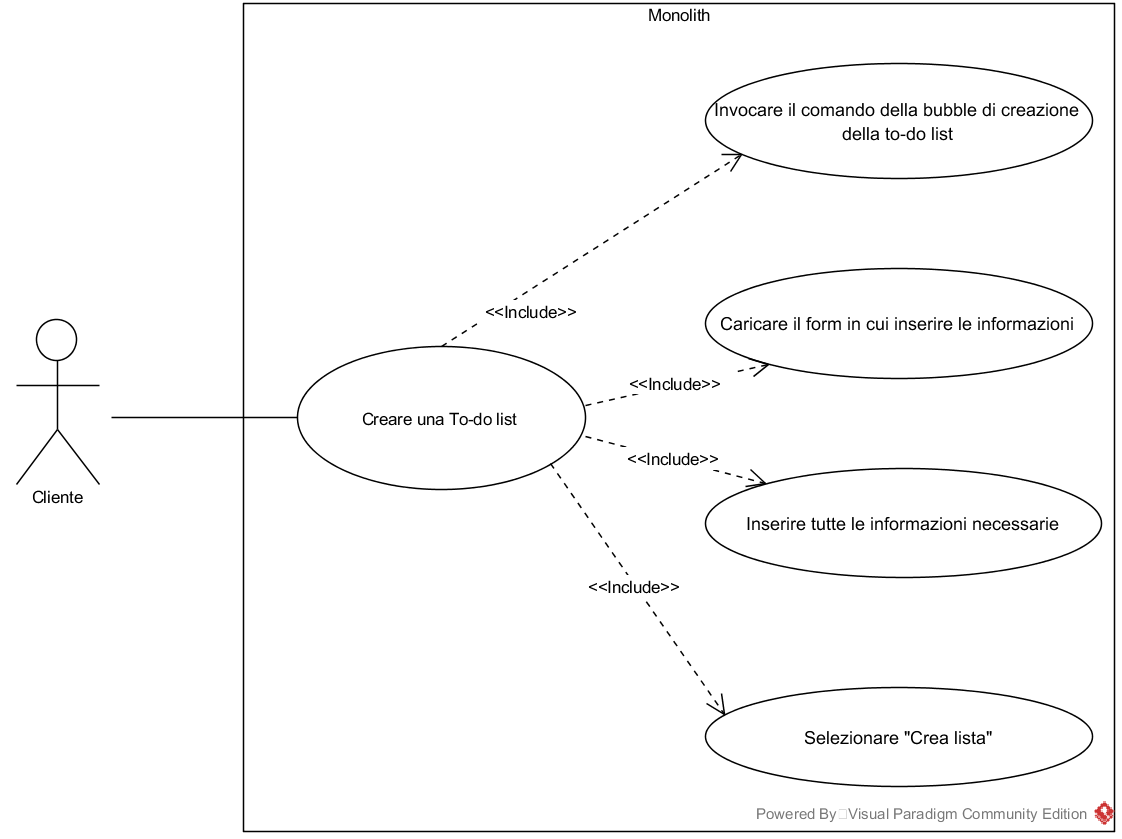
\includegraphics[width=15cm]{../../documenti/AnalisiDeiRequisiti/Diagrammi_img/uc2_1.png}
	\caption{\UCCaption{} Creare una lista}
\end{figure}

\begin{itemize}
	\item \textbf{Attori:}
	\\Utente di Rocket.Chat in possesso di \ProjectName{}.
	\item \textbf{Scopo e descrizione:} 
	\\Creare una lista di cose da fare.
	\item \textbf{Precondizioni:}
	\begin{itemize}
		\item Essere utenti di Rocket.Chat;
		\item Avere \ProjectName{} installato.
	\end{itemize}
	\item \textbf{Flusso principale degli eventi:}
	\begin{itemize}
		\item L'utente invoca il comando di creazione della bubble To-do list \ref{UC2.1.1};
		\item L'utente carica il form in cui inserire le informazioni \ref{UC2.1.2};
		\item L'utente inserisce tutte le informazioni necessarie \ref{UC2.1.3};
		\item L'utente seleziona \virgolette{Crea lista} \ref{UC2.1.4}.
	\end{itemize}
	\item \textbf{Post-condizione:}
	\\Nella conversazione è presente una bubble To-do list con il titolo indicato.
\end{itemize}

\UCF{Invocare il comando della bubble di creazione della to-do list}{UC2.1.1}

\begin{itemize}
	\item \textbf{Attori:}
	\\Utente di Rocket.Chat in possesso di \ProjectName{}.
	\item \textbf{Scopo e descrizione:} 
	\\Creare una to-do list all'interno della chat.
	\item \textbf{Precondizioni:}
	\begin{itemize}
		\item Essere utenti di Rocket.Chat;
		\item Avere \ProjectName{} installato;
		\item Avere accesso alla bubble To-do list.
	\end{itemize}
	\item \textbf{Flusso principale degli eventi:}
	\\L'utilizzatore di \ProjectName{} utilizzando l'apposito comando inizia la creazione della bubble To-do list.
	\item \textbf{Post-condizione:}
	\\Viene istanziata la bubble.
\end{itemize}

\UCF{Caricare il form in cui inserire le informazioni}{UC2.1.2}

\begin{itemize}
	\item \textbf{Attori:}
	\\Utente di Rocket.Chat in possesso di \ProjectName{}.
	\item \textbf{Scopo e descrizione:} 
	\\Creare una to-do list all'interno della chat.
	\item \textbf{Precondizioni:}
	\begin{itemize}
		\item Essere utenti di Rocket.Chat;
		\item Avere \ProjectName{} installato;
		\item Aver invocato il comando di creazione della to-do list \ref{UC2.1.1}.
	\end{itemize}
	\item \textbf{Flusso principale degli eventi:}
	\\Viene caricato il form per l'inserimento delle informazioni.
	\item \textbf{Post-condizione:}
	\\Nella conversazione è presente una bubble To-do list con al suo interno un form per l'inserimento delle informazioni necessarie al completamento della creazione della to-do list.
\end{itemize}

\UCF{Inserire tutte le informazioni necessarie}{UC2.1.3}

\begin{itemize}
	\item \textbf{Attori:}
	\\Utente di Rocket.Chat in possesso di \ProjectName{}.
	\item \textbf{Scopo e descrizione:} 
	\\Specificare le informazioni necessarie alla creazione della lista.
	\item \textbf{Precondizioni:}
	\begin{itemize}
		\item Essere utenti di Rocket.Chat;
		\item Avere \ProjectName{} installato;
		\item Aver caricato il form di inserimento secondo \ref{UC2.1.2}.
	\end{itemize}
	\item \textbf{Flusso principale degli eventi:}
	\\L'utilizzatore della bubble inserisce i dati necessari nel form visualizzato al caso d'uso \ref{UC2.1.2}.
	\item \textbf{Post-condizione:}
	\\Nella memoria della bubble sono salvati i dati richiesti nel caso d'uso \ref{UC2.1.4}. 
\end{itemize}

\UCF{Selezionare \virgolette{Crea lista}}{UC2.1.4}

\begin{itemize}
	\item \textbf{Attori:}
	\\Utente di Rocket.Chat in possesso di \ProjectName{}.
	\item \textbf{Scopo e descrizione:} 
	\\Creazione di una lista di cose da fare.
	\item \textbf{Precondizioni:}
	\begin{itemize}
		\item Essere utenti di Rocket.Chat;
		\item Avere \ProjectName{} installato;
		\item Sono stati inseriti i dati come da \ref{UC2.1.3}.
	\end{itemize}
	\item \textbf{Flusso principale degli eventi:}
	\\Viene utilizzato l'apposito comando per la creazione effettiva della lista all'interno della bubble.
	\item \textbf{Post-condizione:}
	\\Nella conversazione è presente una bubble To-do list con il titolo indicato. 
\end{itemize}

\UC{Aggiungere elemento alla to-do list}{UC2.2}

\begin{figure}[H]
	\centering
	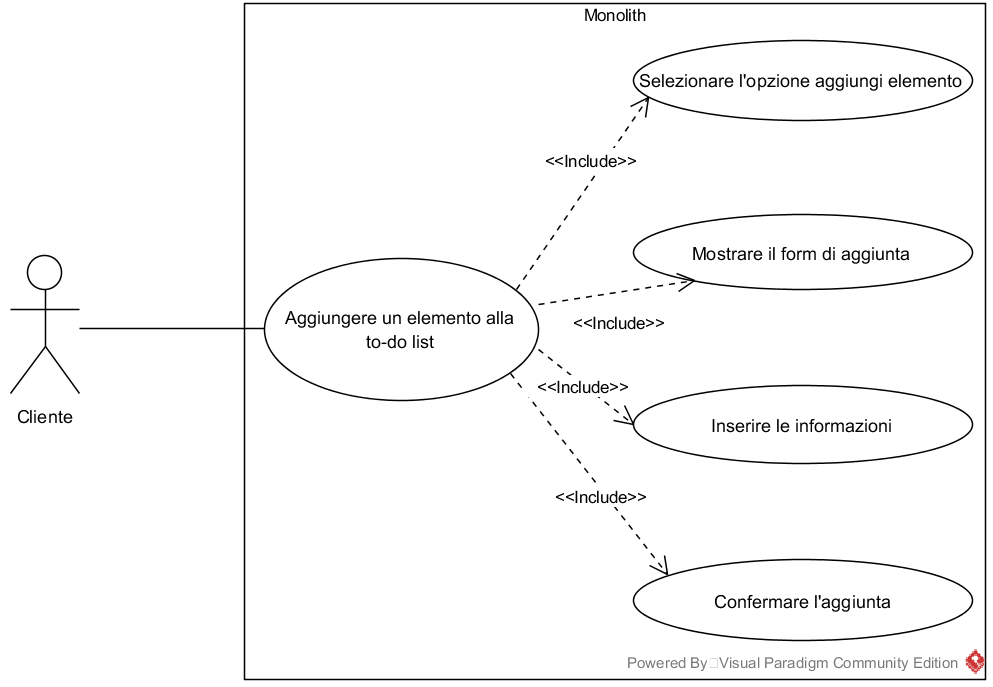
\includegraphics[width=15cm]{../../documenti/AnalisiDeiRequisiti/Diagrammi_img/uc2_2.png}
	\caption{\UCCaption{} Aggiungere elemento alla to-do list}
\end{figure}

\begin{itemize}
	\item \textbf{Attori:}
	\\Utente di Rocket.Chat in possesso di \ProjectName{}.
	\item \textbf{Scopo e descrizione:} 
	\\Un utente inserisce un nuovo elemento\footnote{Sono considerati elementi per la to-do list le voci testuali e/o con immagini.} alla to-do list.
	\item \textbf{Precondizioni:}
	\begin{itemize}
		\item Avere ricevuto una bubble To-do list;
		\item L'elemento non è già stato completato.
	\end{itemize}
	\item \textbf{Flusso principale degli eventi:}
	\begin{itemize}
		\item L'utente seleziona l'opzione aggiungi elemento \ref{UC2.2.1};
		\item Mostrare il form di aggiunta \ref{UC2.2.2};
		\item L'utente inserisce le informazioni \ref{UC2.2.3};
		\item L'utente conferma l'aggiunta \ref{UC2.2.4}.
	\end{itemize}
	\item \textbf{Post-condizione:}
	\\La to-do list avrà il nuovo elemento aggiunto.
\end{itemize}

\UCF{Selezionare l'opzione aggiungi elemento}{UC2.2.1}

\begin{itemize}
	\item \textbf{Attori:}
	\\Utente di Rocket.Chat in possesso di \ProjectName{}.
	\item \textbf{Scopo e descrizione:} 
	\\L'utente seleziona l'opzione per inserire un nuovo elemento alla to-do list.
	\item \textbf{Precondizioni:}
	\begin{itemize}
		\item Avere ricevuto una bubble To-do list.
	\end{itemize}
	\item \textbf{Flusso principale degli eventi:}
	\\L'utilizzatore del metodo seleziona l'opzione apposita.
	\item \textbf{Post-condizione:}
	\\È possibile inserire il testo per il nuovo elemento. 
\end{itemize}

\UCF{Mostrare il form di aggiunta}{UC2.2.2}

\begin{itemize}
	\item \textbf{Attori:}
	\\Utente di Rocket.Chat in possesso di \ProjectName{}.
	\item \textbf{Scopo e descrizione:} 
	\\Visualizzazione del form di aggiunta delle informazioni relative al nuovo elemento della to-do list.
	\item \textbf{Precondizioni:}
	\begin{itemize}
		\item Avere ricevuto una bubble To-do list;
		\item Avere selezionato l'opzione aggiungi elemento come da \ref{UC2.2.1}.
	\end{itemize}
	\item \textbf{Flusso principale degli eventi:}
	\\L'utilizzatore del metodo scrive il testo da inserire nel nuovo elemento e lo aggiunge alla to-do list.
	\item \textbf{Post-condizione:}
	\\Il nuovo elemento è aggiunto alla bubble To-do list.
\end{itemize}

\UCF{Inserire le informazioni}{UC2.2.3}

\begin{itemize}
	\item \textbf{Attori:}
	\\Utente di Rocket.Chat in possesso di \ProjectName{}.
	\item \textbf{Scopo e descrizione:} 
	\\L'utente inserisce le informazioni necessarie ad aggiungere un elemento alla to-do list.
	\item \textbf{Precondizioni:}
	\begin{itemize}
		\item Avere ricevuto una bubble To-do list;
		\item Aver caricato il form di inserimento secondo \ref{UC2.2.2};
	\end{itemize}
	\item \textbf{Flusso principale degli eventi:}
	\\L'utilizzatore del metodo completa il form di inserimento di un nuovo elemento in tutte le sue parti.
	\item \textbf{Post-condizione:}
	\\La to-do list ha tutte le informazioni necessarie per aggiungere il nuovo elemento.
\end{itemize}

\UCF{Confermare l'aggiunta}{UC2.2.4}

\begin{itemize}
	\item \textbf{Attori:}
	\\Utente di Rocket.Chat in possesso di \ProjectName{}.
	\item \textbf{Scopo e descrizione:} 
	\\Un utente conferma l'inserimento del nuovo elemento alla to-do list.
	\item \textbf{Precondizioni:}
	\begin{itemize}
		\item Avere ricevuto una bubble To-do list;
		\item Aver inserito le informazioni per il nuovo elemento secondo \ref{UC2.2.3}.
	\end{itemize}
	\item \textbf{Flusso principale degli eventi:}
	\\L'utilizzatore del metodo conferma l'aggiunta alla to-do list.
	\item \textbf{Post-condizione:}
	\\L'elemento è stato aggiunto alla to-do list.
\end{itemize}

\UC{Indicare come completati gli elementi della to-do list}{UC2.3}

\begin{figure}[H]
	\centering
	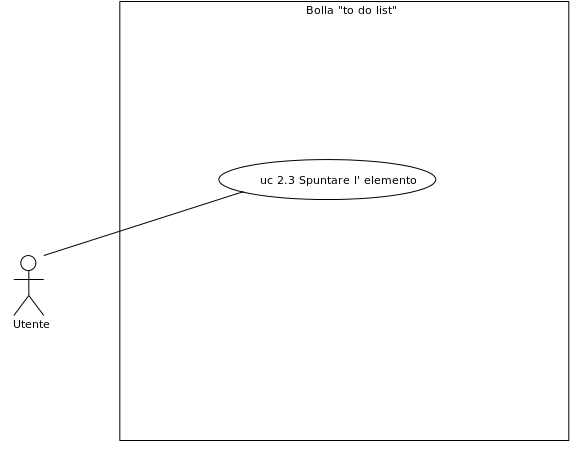
\includegraphics[width=15cm]{../../documenti/AnalisiDeiRequisiti/Diagrammi_img/uc2_3.png}
	\caption{\UCCaption{} Indicare come completati gli elementi della to-do list}
\end{figure}

\begin{itemize}
	\item \textbf{Attori:}
	\\Utente di Rocket.Chat in possesso di \ProjectName{} che abbia ricevuto come messaggio una bubble To-do list.
	\item \textbf{Scopo e descrizione:} 
	\\L'utente con questo metodo può indicare come completato uno degli elementi della lista.
	\item \textbf{Precondizioni:}
	\begin{itemize}
		\item Avere ricevuto una bubble To-do list;
		\item L'elemento non è già stato completato.
	\end{itemize}
	\item \textbf{Flusso principale degli eventi:}
	\\L'utilizzatore del metodo seleziona un elemento della to-do list e lo indica come completato. 
	\item \textbf{Post-condizione:}
	\\L'elemento della to-do list viene aggiornato come completato.
\end{itemize}

\UC{Possibilità di mettere un reminder come notifica statica}{UC2.4}

\begin{figure}[H]
	\centering
	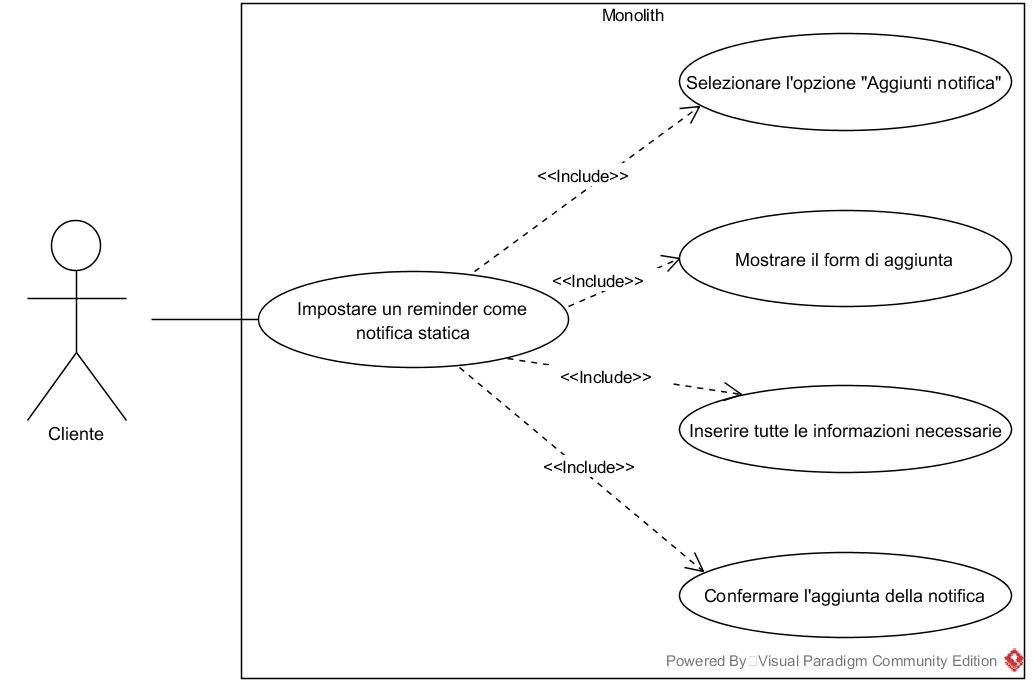
\includegraphics[width=15cm]{../../documenti/AnalisiDeiRequisiti/Diagrammi_img/uc2_4.png}
	\caption{\UCCaption{} Possibilità di mettere un reminder come notifica statica}
\end{figure}

\begin{itemize}
	\item \textbf{Attori:}
	\\Utente di Rocket.Chat in possesso di \ProjectName{} che ha creato la to-do list.
	\item \textbf{Scopo e descrizione:} 
	\\Il creatore della lista imposta una notifica statica da visualizzare ai membri del canale ad un orario specificato.
	\item \textbf{Precondizioni:}
	\begin{itemize}
		\item Avere ricevuto una bubble To-do list.
	\end{itemize}
	\item \textbf{Flusso principale degli eventi:}
	\begin{itemize}
		\item L'utente seleziona l'opzione aggiungi notifica \ref{UC2.4.1};
		\item Mostrare il form di aggiunta \ref{UC2.4.2};
		\item L'utente inserisce tutte le informazioni necessarie \ref{UC2.4.3};
		\item L'utente conferma l'aggiunta della notifica \ref{UC2.4.4}.
	\end{itemize}
	\item \textbf{Post-condizione:}
	\\I partecipanti al gruppo nel quale è presente la bubble verranno notificati della lista all'ora specificata.
\end{itemize}

\UCF{Selezionare l'opzione aggiungi notifica}{UC2.4.1}

\begin{itemize}
	\item \textbf{Attori:}
	\\Utente di Rocket.Chat in possesso di \ProjectName{}.
	\item \textbf{Scopo e descrizione:} 
	\\Il creatore della lista seleziona l'opzione \virgolette{aggiungi notifica} per la to-do list che ha creato.
	\item \textbf{Precondizioni:}
	\begin{itemize}
		\item Avere creato una bubble To-do list.
	\end{itemize}
	\item \textbf{Flusso principale degli eventi:}
	\\L'utilizzatore del metodo seleziona l'opzione \virgolette{aggiungi notifica} sulla bubble.
	\item \textbf{Post-condizione:}
	\\L'utente ha selezionato l'opzione di aggiungere una notifica alla to-do list che ha creato.
\end{itemize}

\UCF{Mostrare il form di aggiunta}{UC2.4.2}

\begin{itemize}
	\item \textbf{Attori:}
	\\Utente di Rocket.Chat in possesso di \ProjectName{}.
	\item \textbf{Scopo e descrizione:} 
	\\Questa funzionalità permette alla bubble di caricare il form necessario ad inserire i dati per aggiungere una notifica alla bubble.
	\item \textbf{Precondizioni:}
	\begin{itemize}
		\item Avere ricevuto una bubble To-do list;
		\item Essere entrati nell'opzione \virgolette{aggiungi modifica} della propria bubble secondo \ref{UC2.4.1}.
	\end{itemize}
	\item \textbf{Flusso principale degli eventi:}
	\\La bubble To-do list carica il form di inserimento dati per le notifiche.
	\item \textbf{Post-condizione:}
	\\La bubble ha caricato il form ed è pronta a ricevere in input le informazioni sulla notifica.
\end{itemize}

\UCF{Inserire tutte le informazioni necessarie}{UC2.4.3}

\begin{itemize}
	\item \textbf{Attori:}
	\\Utente di Rocket.Chat in possesso di monolith.
	\item \textbf{Scopo e descrizione:} 
	\\Il creatore della lista completa il form di aggiunta notifica.
	\item \textbf{Precondizioni:}
	\begin{itemize}
		\item Avere ricevuto una bubble di to-do list;
		\item La bubble ha caricato il form di inserimento dati secondo lo \ref{UC2.4.2}.
	\end{itemize}
	\item \textbf{Flusso principale degli eventi:}
	\\L'utilizzatore del metodo inserirà tutte le informazioni necessarie a completare il form di aggiunta di una notifica.
	\item \textbf{Post-condizione:}
	\\La bubble possiede tutte le informazioni necessarie ad aggiungere una notifica alla to-do list.
\end{itemize}

\UCF{Confermare l'aggiunta della notifica}{UC2.4.4}

\begin{itemize}
	\item \textbf{Attori:}
	\\Utente di Rocket.Chat in possesso di \ProjectName{}.
	\item \textbf{Scopo e descrizione:} 
	\\Il creatore della lista conferma l'aggiunta della notifica.
	\item \textbf{Precondizioni:}
	\begin{itemize}
		\item Avere ricevuto una bubble To-do list;
		\item Aver completato il form di aggiunta di una notifica secondo lo \ref{UC2.4.3}.
	\end{itemize}
	\item \textbf{Flusso principale degli eventi:}
	\\L'utilizzatore del metodo seleziona l'opzione \virgolette{conferma aggiunta} e la bubble aggiunge la notifica alla lista.
	\item \textbf{Post-condizione:}
	\\La bubble ha aggiunto la notifica alla to-do list.
\end{itemize}

\subsection{Bubble \& eat - Cliente}

\UC{Registrazione dei propri dati personali}{UC3.1}

\begin{figure}[H]
	\centering
	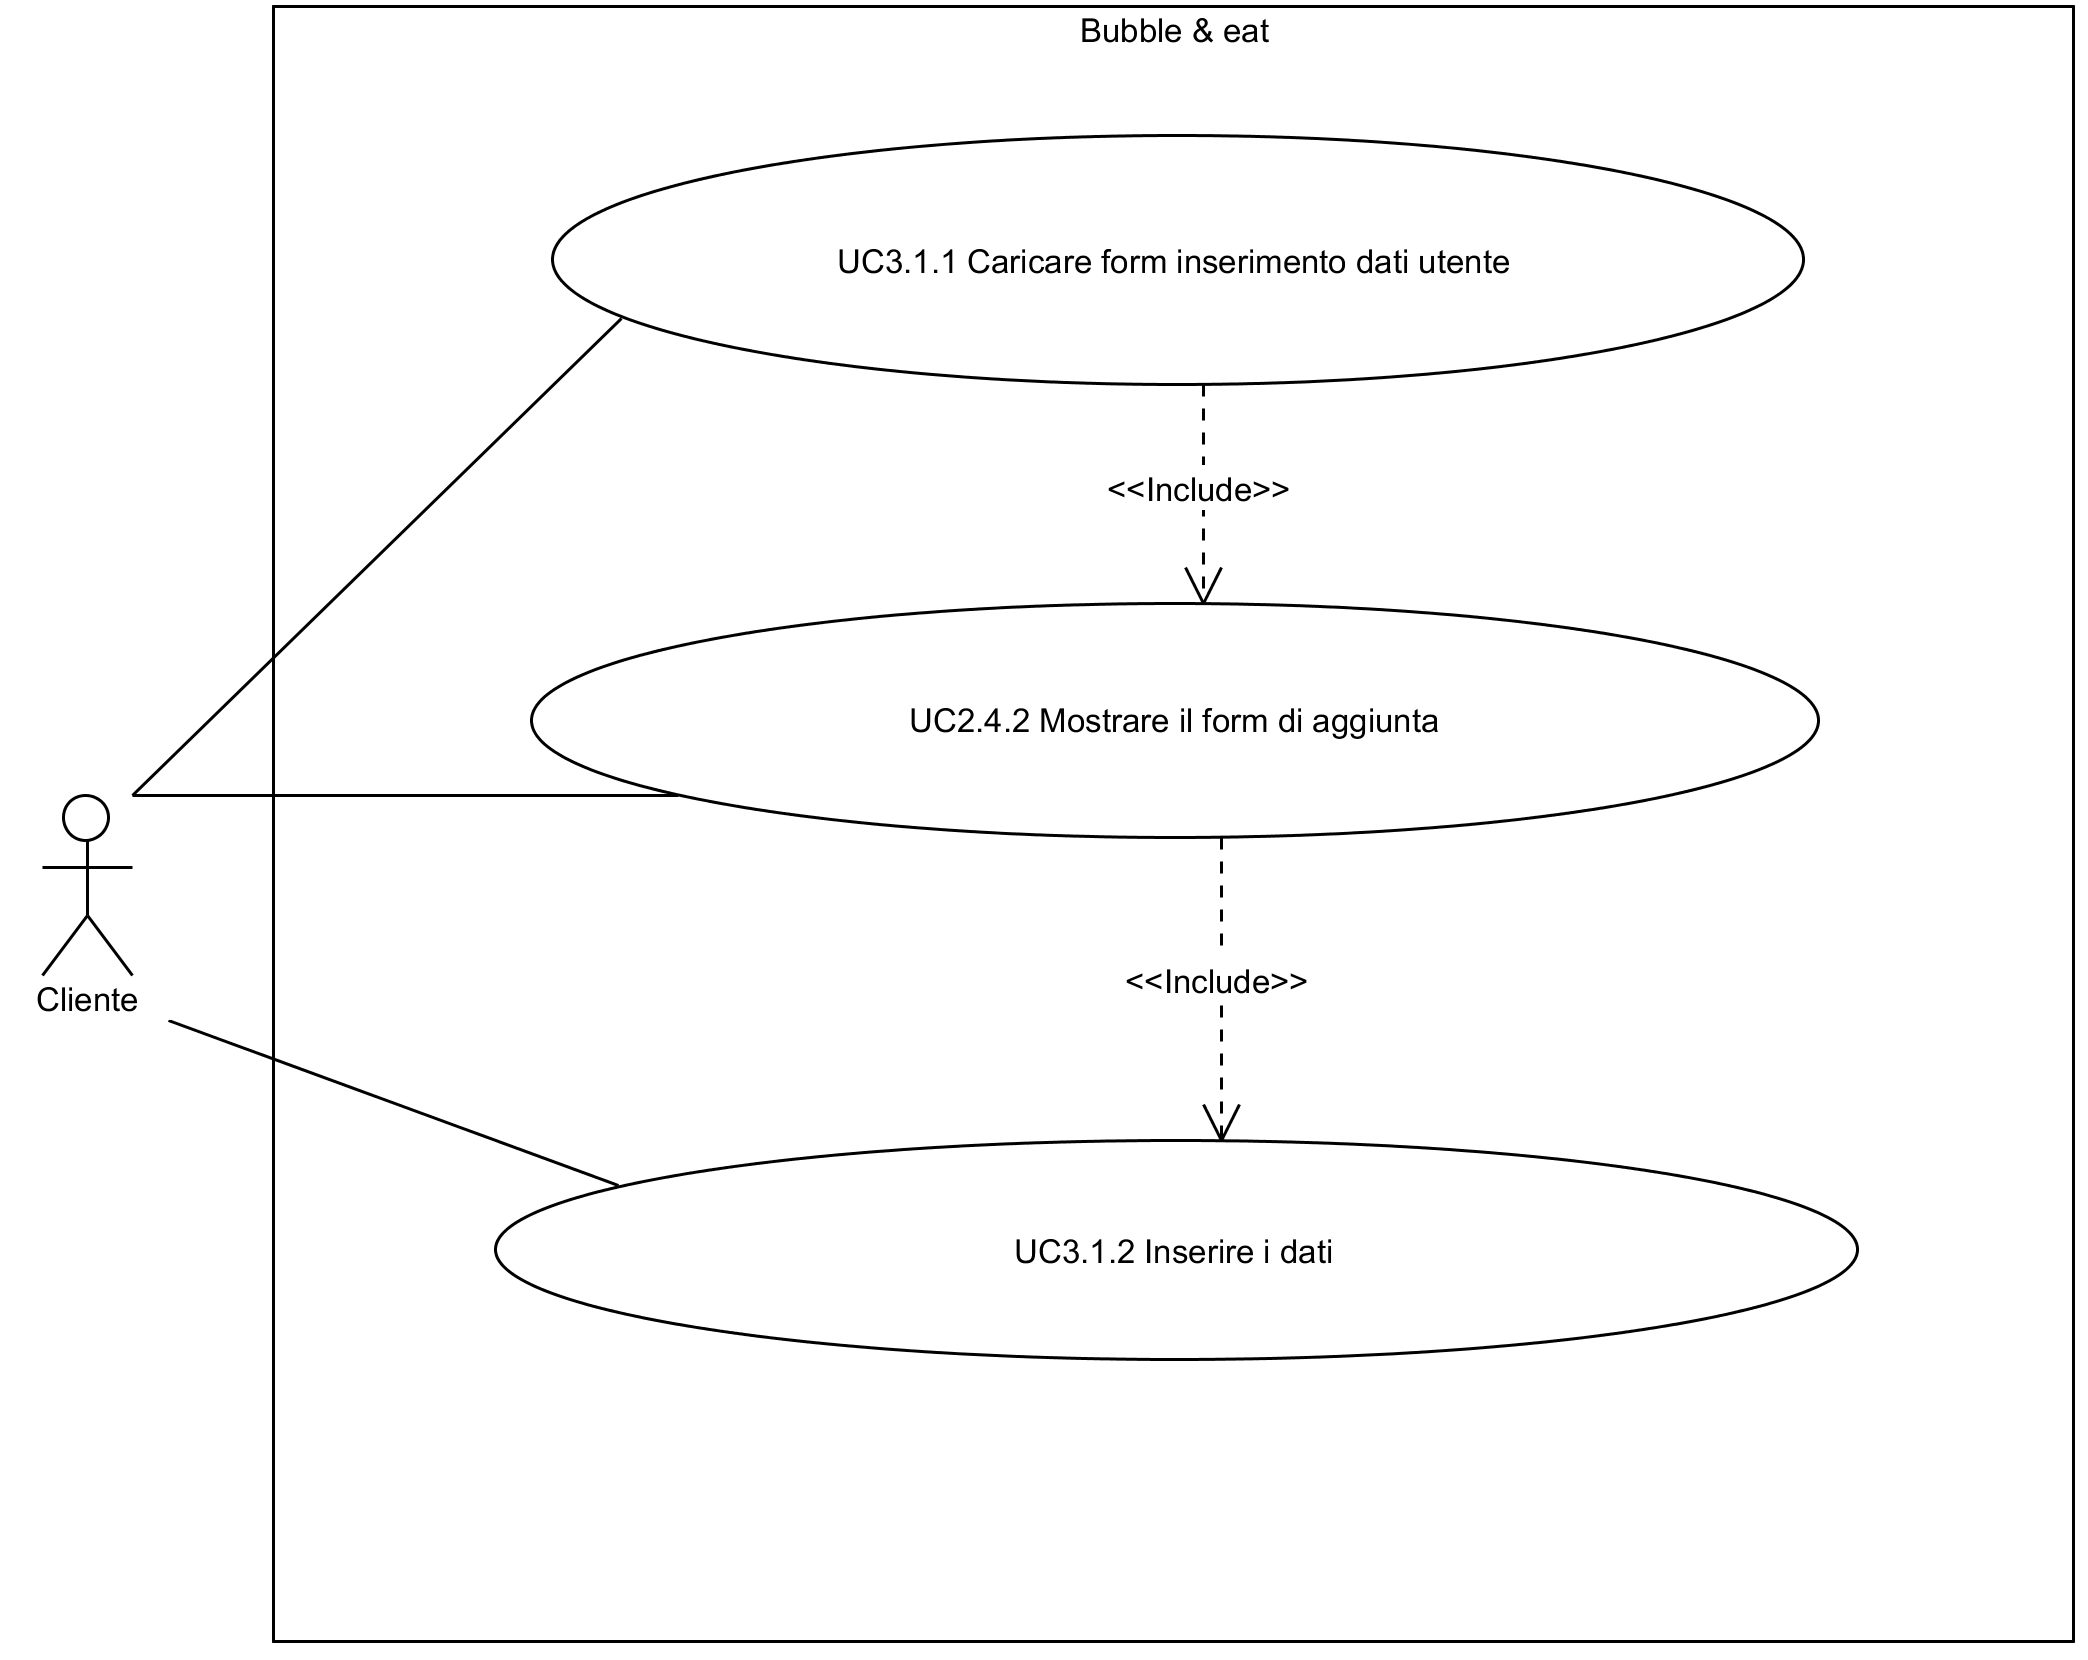
\includegraphics[width=15cm]{../../documenti/AnalisiDeiRequisiti/Diagrammi_img/uc3_1.png}
	\caption{\UCCaption{} Registrazione dei propri dati personali}
\end{figure}

\begin{itemize}
	\item \textbf{Attori:}
	\\Cliente.
	\item \textbf{Scopo e descrizione:} 
	\\Registrare il proprio indirizzo e il proprio nome e cognome in modo tale da segnalarli all'azienda come destinazione per la spedizione del cibo.
	\item \textbf{Precondizioni:}
	\begin{itemize}
		\item Avere Rocket.Chat;
		\item Avere la bubble del ristorante selezionato.
	\end{itemize}
	\item \textbf{Flusso principale degli eventi:}
	\begin{itemize}
		\item Viene caricato il form di inserimento dati dell'utente \ref{UC3.1.1};
		\item L'utente inserisce i dati \ref{UC3.1.2};
		\item L'utente conferma l'inserimento \ref{UC3.1.3}.
	\end{itemize}
	\item \textbf{Post-condizione:}
	\\I dati dell'utente sono stati registrati nella bubble memory.
\end{itemize}

\UCF{Caricare form inserimento dati utente}{UC3.1.1}

\begin{itemize}
	\item \textbf{Attori:}
	\\Cliente.
	\item \textbf{Scopo e descrizione:} 
	\\Dare la possibilità di inserire i propri dati con lo scopo di segnalarli al locale per il corretto funzionamento del servizio.
	\item \textbf{Precondizioni:}
	\begin{itemize}
		\item Avere Rocket.Chat;
		\item Avere la bubble del ristorante selezionato.
	\end{itemize}
	\item \textbf{Flusso principale degli eventi:}
	\\Il form per l'inserimento dei dati utente viene caricato.
	\item \textbf{Post-condizione:}
	\\Nella bubble è presente il form per l'inserimento dei dati.
\end{itemize}

\UCF{Inserire i dati}{UC3.1.2}

\begin{itemize}
	\item \textbf{Attori:}
	\\Cliente.
	\item \textbf{Scopo e descrizione:} 
	\\Questo metodo permette all'utente di inserire il proprio indirizzo e il proprio nome e cognome con il fine di segnalarlo all'azienda, in modo tale da avere una destinazione per la spedizione del cibo.
	\item \textbf{Precondizioni:}
	\begin{itemize}
		\item Avere Rocket.Chat;
		\item Avere la bubble del ristorante selezionato.
	\end{itemize}
	\item \textbf{Flusso principale degli eventi:}
	\\L'utente seleziona i campi del form di inserimento e digita le informazioni.
	\item \textbf{Post-condizione:}
	\\I dati dell'utente sono stati inseriti.
\end{itemize}

\UCF{Conferma inserimento}{UC3.1.3}

\begin{itemize}
	\item \textbf{Attori:}
	\\Cliente.
	\item \textbf{Scopo e descrizione:} 
	\\Questo metodo permette all'utente di confermare l'inserimento dei dati inseriti nel form di registrazione.
	\item \textbf{Precondizioni:}
	\begin{itemize}
		\item Avere Rocket.Chat;
		\item Avere la bubble del ristorante selezionato.
	\end{itemize}
	\item \textbf{Flusso principale degli eventi:}
	\\Con l'apposito comando il Cliente conferma che i dati precedentemente immessi al caso d'uso \ref{UC3.1.2} siano corretti.
	\item \textbf{Post-condizione:}
	\\I dati confermati sono presenti nella memoria della bubble.
\end{itemize}

\UC{Guardare il menù}{UC3.2}

\begin{figure}[H]
	\centering
	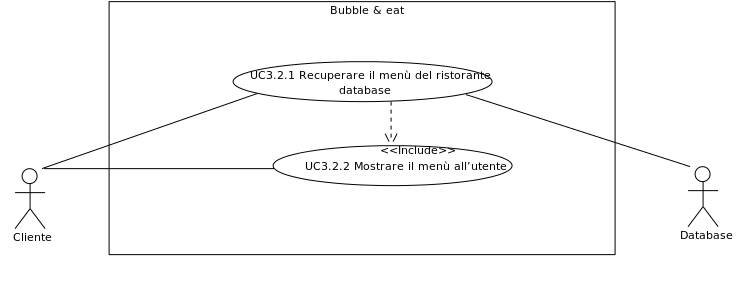
\includegraphics[width=15cm]{../../documenti/AnalisiDeiRequisiti/Diagrammi_img/uc3_2.png}
	\caption{\UCCaption{} Guardare il menù}
\end{figure}

\begin{itemize}
	\item \textbf{Attori:}
	\\Cliente.
	\item \textbf{Scopo e descrizione:} 
	\\Il Cliente consulta il menù.
	\item \textbf{Precondizioni:}
	\begin{itemize}
		\item Avere Rocket.Chat;
		\item Avere la bubble del ristorante selezionato;
		\item Essere loggato nella bubble.
	\end{itemize}
	\item \textbf{Flusso principale degli eventi:}
	\begin{itemize}
		\item Viene recuperato il menù del ristorante dal database \ref{UC3.2.1};
		\item Il menù caricato viene mostrato all'utente \ref{UC3.2.2}.
	\end{itemize}
	\item \textbf{Post-condizione:}
	\\Il menù è visualizzato sulla bubble.
\end{itemize}

\UCF{Recuperare il menù del ristorante dal database}{UC3.2.1}

\begin{itemize}
	\item \textbf{Attori:}
	\\Cliente.
	\item \textbf{Scopo e descrizione:} 
	\\Recuperare dal database le voci del menù del ristorante.
	\item \textbf{Precondizioni:}
	\begin{itemize}
		\item Avere Rocket.Chat;
		\item Avere la bubble del ristorante selezionato;
		\item Essere loggato nella bubble.
	\end{itemize}
	\item \textbf{Flusso principale degli eventi:}
	\\L'utente invia la richiesta di visualizzazione del menù e la bubble lo carica dal database.
	\item \textbf{Post-condizione:}
	\\Le informazioni sul menù sono state recuperate dalla bubble.
\end{itemize}

\UCF{Mostrare il menù all'utente}{UC3.2.2}

\begin{itemize}
	\item \textbf{Attori:}
	\\Cliente.
	\item \textbf{Scopo e descrizione:} 
	\\Visualizzare il menù nella bubble.
	\item \textbf{Precondizioni:}
	\begin{itemize}
		\item Avere Rocket.Chat;
		\item Avere la bubble del ristorante selezionato;
		\item Essere loggato nella bubble.
	\end{itemize}
	\item \textbf{Flusso principale degli eventi:}
	\\Il menù viene mostrato all'utente.
	\item \textbf{Post-condizione:}
	\\Il menù è visualizzato sulla bubble.
\end{itemize}

\UC{Fare le ordinazioni}{UC3.3}

\begin{figure}[H]
	\centering
	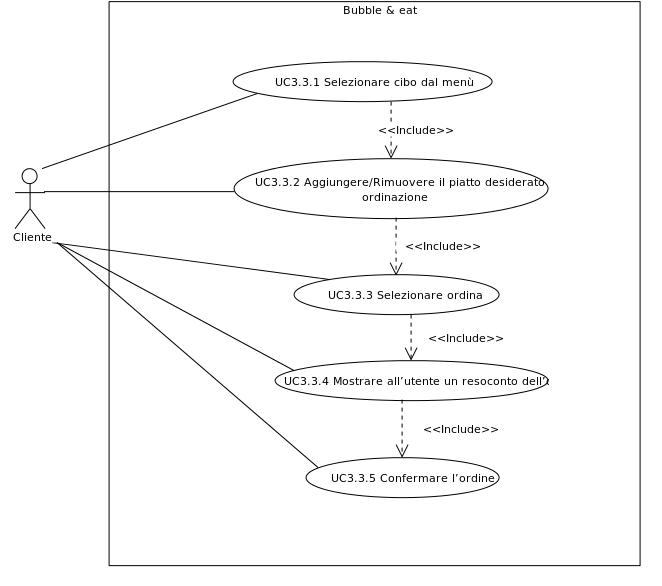
\includegraphics[width=15cm]{../../documenti/AnalisiDeiRequisiti/Diagrammi_img/uc3_3.png}
	\caption{UC3.3 Fare le ordinazioni}
\end{figure}

\begin{itemize}
	\item \textbf{Attori:}
	\\Cliente.
	\item \textbf{Scopo e descrizione:} 
	\\Selezionare i piatti e le quantità relative ad ogni pietanza.
	\item \textbf{Precondizioni:}
	\begin{itemize}
		\item Avere Rocket.Chat;
		\item Avere la bubble del ristorante selezionato;
		\item Essere loggato nella bubble.
	\end{itemize}
	\item \textbf{Flusso principale degli eventi:}
	\begin{itemize}
		\item Visualizzare menù \ref{UC3.2};
		\item Selezionare cibi dal menù \ref{UC3.3.1};
		\item Aggiungere/Rimuovere il cibo selezionato all'ordine \ref{UC3.3.2};
		\item Selezionare \virgolette{Ordina} \ref{UC3.3.3};
		\item Mostrare all'utente un resoconto dell'ordine \ref{UC3.3.4};
		\item Confermare l'ordine \ref{UC3.3.5}.
	\end{itemize}
	\item \textbf{Post-condizione:}
	\\L'ordinazione viene aggiornata.
\end{itemize}

\UCF{Selezionare cibo dal menù}{UC3.3.1}

\begin{itemize}
	\item \textbf{Attori:}
	\\Cliente.
	\item \textbf{Scopo e descrizione:} 
	\\Selezionare voce di menù e relativa quantità.
	\item \textbf{Precondizioni:}
	\begin{itemize}
		\item Avere Rocket.Chat;
		\item Avere la bubble del ristorante selezionato;
		\item Essere loggato nella bubble;
		\item Aver caricato il menù del ristorante \ref{UC3.2}.
	\end{itemize}
	\item \textbf{Flusso principale degli eventi:}
	\begin{itemize}
		\item L'utente scorre la lista dei cibi ne seleziona voci e relative quantità.
	\end{itemize}
	\item \textbf{Post-condizione:}
	\\L'utente ha selezionato almeno un piatto dal menù.
\end{itemize}

\UCF{Aggiungere/Rimuovere il piatto desiderato dall'ordinazione}{UC3.3.2}

\begin{itemize}
	\item \textbf{Attori:}
	\\Cliente.
	\item \textbf{Scopo e descrizione:} 
	\\Aggiungere oppure rimuovere alla propria ordinazione un'unità del piatto selezionato.
	\item \textbf{Precondizioni:}
	\begin{itemize}
		\item Avere Rocket.Chat;
		\item Avere la bubble del ristorante selezionato;
		\item Essere loggato nella bubble.
	\end{itemize}
	\item \textbf{Flusso principale degli eventi:}
	\\L'utente invoca l'apposito comando sulla bubble per poter rimuovere o aggiungere il piatto selezionato al proprio ordine.
	\item \textbf{Post-condizione:}
	\\L'ordinazione viene aggiornata correttamente con il piatto selezionato.
\end{itemize}

\UCF{Selezionare \virgolette{Ordina}}{UC3.3.3}

\begin{itemize}
	\item \textbf{Attori:}
	\\Cliente.
	\item \textbf{Scopo e descrizione:} 
	\\Il Cliente effettua l'ordine selezionando l'apposita funzione.
	\item \textbf{Precondizioni:}
	\begin{itemize}
		\item Avere Rocket.Chat;
		\item Avere la bubble del ristorante selezionato;
		\item Essere loggato nella bubble;
		\item Aver selezionato cibi e quantità dal menù \ref{UC3.3.1} \ref{UC3.3.2}.
	\end{itemize}
	\item \textbf{Flusso principale degli eventi:}
	\\L'utente invoca l'apposito comando di ordine sulla bubble.
	\item \textbf{Post-condizione:}
	\\L'ordinazione è registrata ed è in attesa di conferma.
\end{itemize}

\UCF{Mostrare all'utente un resoconto dell'ordine}{UC3.3.4}

\begin{itemize}
	\item \textbf{Attori:}
	\\Cliente.
	\item \textbf{Scopo e descrizione:} 
	\\Mostrare all'utente un resoconto dell'ordine che sta per effettuare prima della conferma.
	\item \textbf{Precondizioni:}
	\begin{itemize}
		\item Avere Rocket.Chat;
		\item Avere la bubble del ristorante selezionato;
		\item Essere loggato nella bubble;
		\item Aver selezionato cibi e quantità dal menù \ref{UC3.3.1} \ref{UC3.3.2}.
	\end{itemize}
	\item \textbf{Flusso principale degli eventi:}
	\\L'utente seleziona \virgolette{Mostra resoconto} e riceve dunque una lista completa di tutto e solo quello che sta per ordinare, insieme al prezzo totale dell'ordine.
	\item \textbf{Post-condizione:}
	\\L'utente visualizza un resoconto dell'ordine prima di confermarlo.
\end{itemize}

\UCF{Confermare l'ordine}{UC3.3.5}

\begin{itemize}
	\item \textbf{Attori:}
	\\Cliente.
	\item \textbf{Scopo e descrizione:} 
	\\Confermare che quanto mostrato nel caso d'uso \ref{UC3.3.4} è corretto e salvare l'ordinazione nella memoria della bubble.
	\item \textbf{Precondizioni:}
	\begin{itemize}
		\item Avere Rocket.Chat;
		\item Avere la bubble del ristorante selezionato;
		\item Essere loggato nella bubble;
		\item Aver effettuato l'ordinazione \ref{UC3.3.4}.
	\end{itemize}
	\item \textbf{Flusso principale degli eventi:}
	\\L'utente invoca l'apposito comando sulla bubble.
	\item \textbf{Post-condizione:}
	\\L'ordinazione viene salvata nella memoria della bubble.
\end{itemize}

\UC{Inviare l'ordinazione}{UC3.4}

\begin{figure}[H]
	\centering
	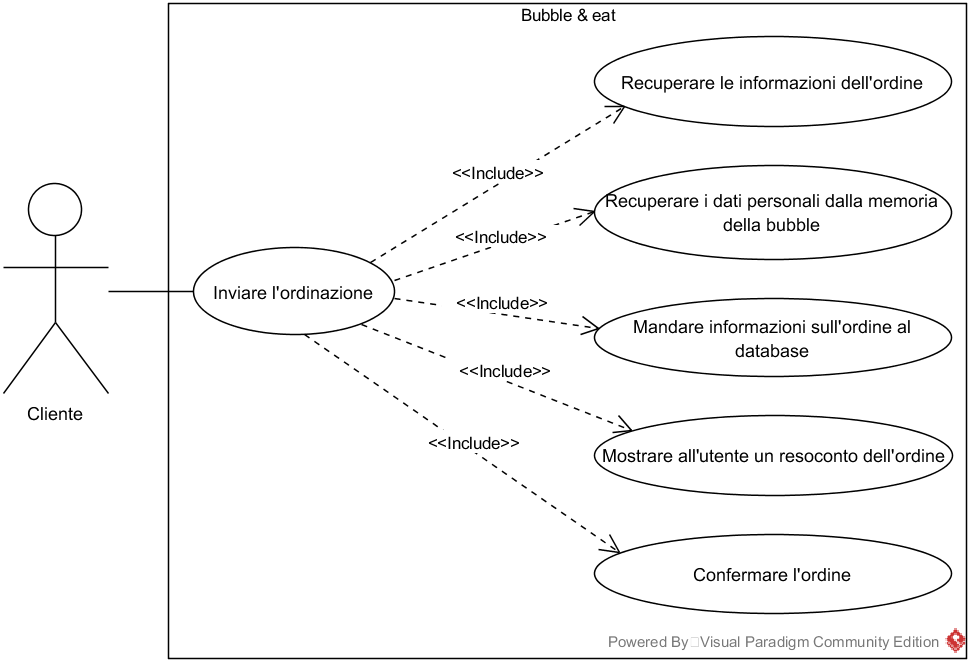
\includegraphics[width=15cm]{../../documenti/AnalisiDeiRequisiti/Diagrammi_img/uc3_4.png}
	\caption{UC3.4 Inviare l'ordinazione}
\end{figure}

\begin{itemize}
	\item \textbf{Attori:}
	\\Cliente.
	\item \textbf{Scopo e descrizione:} 
	\\Selezionare il comando di invio dell'ordinazione.
	\item \textbf{Precondizioni:}
	\begin{itemize}
		\item Avere Rocket.Chat;
		\item Avere la bubble del ristorante selezionato;
		\item Essere loggato nella bubble;
		\item Avere un'ordinazione non vuota.
	\end{itemize}
	\item \textbf{Flusso principale degli eventi:}
	\begin{itemize}
		\item Vengono recuperate dalla memoria della bubble le informazioni sull'ordine \ref{UC3.4.1};
		\item Vengono recuperate le informazioni sui dati personali del Cliente dalla memoria della bubble \ref{UC3.4.2};
		\item Vengono inviate le informazioni sull'ordine al database \ref{UC3.4.3}.
	\end{itemize}
	\item \textbf{Post-condizione:}
	\\L'ordinazione viene inviata.
\end{itemize}

\UCF{Recuperare le informazioni dell'ordine}{UC3.4.1}

\begin{itemize}
	\item \textbf{Attori:}
	\\Cliente.
	\item \textbf{Scopo e descrizione:} 
	\\Prelevare dalla memoria della bubble i dati relativi all'ordinazione confermata nell'\ref{UC3.3.5}.
	\item \textbf{Precondizioni:}
	\begin{itemize}
		\item \ref{UC3.3.5};
		\item Avere Rocket.Chat;
		\item Avere la bubble del ristorante selezionato;
		\item Essere loggato nella bubble.
	\end{itemize}
	\item \textbf{Flusso principale degli eventi:}
	\\L'utente invoca con l'apposito comando l'\ref{UC3.4}.
	\item \textbf{Post-condizione:}
	\\I dati desiderati, relativi all'ordinazione effettuata nell'\ref{UC3.3}, sono stati recuperati. 
\end{itemize}

\UCF{Recuperare informazioni dei dati personali dalla memoria della bubble}{UC3.4.2}

\begin{itemize}
	\item \textbf{Attori:}
	\\Cliente.
	\item \textbf{Scopo e descrizione:} 
	\\Ottenere informazioni riguardanti il Cliente dalla memoria della bubble.
	\item \textbf{Precondizioni:}
	\begin{itemize}
		\item Avere Rocket.Chat;
		\item Avere la bubble del ristorante selezionato;
		\item Essere loggato nella bubble;
		\item Avere un'ordinazione da inviare non vuota.
	\end{itemize}
	\item \textbf{Flusso principale degli eventi:}
	\\Vengono recuperate le informazioni sui dati personali del Cliente dalla memoria della bubble.
	\item \textbf{Post-condizione:}
	\\I dati personali del Cliente sono stati letti dalla memoria della bubble.
\end{itemize}

\UCF{Mandare informazioni sull'ordine al database}{UC3.4.3}

\begin{itemize}
	\item \textbf{Attori:}
	\\Cliente.
	\item \textbf{Scopo e descrizione:} 
	\\Invio delle informazioni al database.
	\item \textbf{Precondizioni:}
	\begin{itemize}
		\item Avere Rocket.Chat;
		\item Avere la bubble del ristorante selezionato;
		\item Essere loggato nella bubble;
		\item Avere un'ordinazione non vuota.
	\end{itemize}
	\item \textbf{Flusso principale degli eventi:}
	\\Le informazioni sull'ordinazione vengono mandate al database.
	\item \textbf{Post-condizione:}
	\\L'ordinazione è salvata nel database.
\end{itemize}

\subsection{Bubble \& eat - Cuoco}

\UC{Leggere la lista dei piatti da preparare}{UC3.5}

\begin{figure}[H]
	\centering
	\includegraphics[width=15cm]{../../documenti/AnalisiDeiRequisiti/Diagrammi_img/uc3_5.png}
	\caption{\UCCaption{} Leggere la lista dei piatti da preparare}
\end{figure}

\begin{itemize}
	\item \textbf{Attori:}
	\\Cuoco.
	\item \textbf{Scopo e descrizione:} 
	\\Lo scopo di questa funzionalità è permettere al Cuoco di consultare la lista dei piatti da preparare ottenuta tramite le ordinazioni effettuate dai clienti.
	\item \textbf{Precondizioni:}
	\begin{itemize}
		\item Avere Rocket.Chat;
		\item Avere la bubble del ristorante selezionato;
		\item Avere accesso alla bubble con il ruolo di Cuoco.
	\end{itemize}
	\item \textbf{Flusso principale degli eventi:}
	\begin{itemize}
		\item Il Cuoco seleziona la parte corrispondente della bubble;
		\item Viene recuperata dal database la lista dei piatti \ref{UC3.5.1};
		\item Viene mostrata la lista all'utente \ref{UC3.5.2}.
	\end{itemize}
	\item \textbf{Post-condizione:}
	\\Il Cuoco è a conoscenza dei piatti ordinati.
\end{itemize}

\UCF{Recuperare dal database la lista dei piatti}{UC3.5.1}

\begin{itemize}
	\item \textbf{Attori:}
	\\Cuoco.
	\item \textbf{Scopo e descrizione:} 
	\\Lo scopo di questa funzionalità è quello di caricare dal database la lista dei piatti da preparare.
	\item \textbf{Precondizioni:}
	\begin{itemize}
		\item Avere Rocket.Chat;
		\item Avere la bubble del ristorante selezionato;
		\item Avere accesso alla bubble con il ruolo di Cuoco.
	\end{itemize}
	\item \textbf{Flusso principale degli eventi:}
	\\Il Cuoco richiede di visualizzare la lista dei piatti da preparare, la bubble carica la lista dal database.
	\item \textbf{Post-condizione:}
	\\La bubble ha recuperato la lista dei piatti da preparare dal database.
\end{itemize}

\UCF{Mostrare la lista}{UC3.5.2}

\begin{itemize}
	\item \textbf{Attori:}
	\\Cuoco.
	\item \textbf{Scopo e descrizione:} 
	\\Lo scopo di questa funzionalità è di far visualizzare al Cuoco la lista dei piatti precedentemente caricata dal database sulla bubble.
	\item \textbf{Precondizioni:}
	\begin{itemize}
		\item Avere Rocket.Chat;
		\item Avere la bubble del ristorante selezionato;
		\item Avere accesso alla bubble con il ruolo di Cuoco;
		\item Aver caricato la lista dei piatti \ref{UC3.5.1}.
	\end{itemize}
	\item \textbf{Flusso principale degli eventi:}
	\\La bubble mostra la lista dei piatti precedentemente memorizzata al Cuoco.
	\item \textbf{Post-condizione:}
	\\Il Cuoco visualizza la lista dei piatti.
\end{itemize}

\UC{Spunta piatti pronti}{UC3.6}

\begin{figure}[H]
	\centering
	\includegraphics[width=15cm]{../../documenti/AnalisiDeiRequisiti/Diagrammi_img/uc3_6.png}
	\caption{\UCCaption{} Spunta piatti pronti}
\end{figure}

\begin{itemize}
	\item \textbf{Attori:}
	\\Cuoco.
	\item \textbf{Scopo e descrizione:} 
	\\I piatti presenti nella lista possono essere spuntati quando il Cuoco ha finito la loro preparazione.
	\item \textbf{Precondizioni:}
	\begin{itemize}
		\item Avere Rocket.Chat;
		\item Avere la bubble del ristorante selezionato;
		\item Avere accesso alla bubble con il ruolo di Cuoco;
		\item Avere la lista dei piatti da preparare.
	\end{itemize}
	\item \textbf{Flusso principale degli eventi:}
	\begin{itemize}
		\item Il Cuoco indica che ha terminato la preparazione di un piatto \ref{UC3.6.1};
		\item Il database viene aggiornato con le nuove informazioni \ref{UC3.6.2}.
	\end{itemize}
	\item \textbf{Post-condizione:}
	\\Il piatto è stato spuntato.
\end{itemize}

\UCF{Indicare che la preparazione del piatto è stata completata}{UC3.6.1}

\begin{itemize}
	\item \textbf{Attori:}
	\\Cuoco.
	\item \textbf{Scopo e descrizione:} 
	\\Lo scopo di questa funzionalità è di permettere al Cuoco di indicare che ha completato la preparazione di un piatto.
	\item \textbf{Precondizioni:}
	\begin{itemize}
		\item Avere Rocket.Chat;
		\item Avere la bubble del ristorante selezionato;
		\item Avere accesso alla bubble con il ruolo di Cuoco;
		\item Avere la lista dei piatti da preparare;
		\item Aver precedentemente indicato che si stava preparando un determinato piatto.
	\end{itemize}
	\item \textbf{Flusso principale degli eventi:}
	\\Il Cuoco indica sulla sua lista che ha completato la preparazione del piatto.
	\item \textbf{Post-condizione:}
	\\Il Cuoco ha indicato che ha completato un piatto.
\end{itemize}

\UCF{Aggiornare il database indicando che il piatto è stato preparato}{UC3.6.2}

\begin{itemize}
	\item \textbf{Attori:}
	\\Cuoco.
	\item \textbf{Scopo e descrizione:} 
	\\Lo scopo di questa funzionalità è quello di aggiornare il database in base ai piatti preparati dal Cuoco.
	\item \textbf{Precondizioni:}
	\begin{itemize}
		\item Avere Rocket.Chat;
		\item Avere la bubble del ristorante selezionato;
		\item Avere accesso alla bubble con il ruolo di Cuoco;
		\item Avere preparato dei piatti dalla lista di piatti da preparare.
	\end{itemize}
	\item \textbf{Flusso principale degli eventi:}
	\\I dati sui piatti preparati dal Cuoco vengono aggiornati nel database.
	\item \textbf{Post-condizione:}
	\\I dati nel database sono aggiornati.
\end{itemize}

\subsection{Bubble \& eat - Responsabile Acquisti}

\UC{Leggere la lista degli acquisti da effettuare}{UC3.7}

\begin{figure}[H]
	\centering
	\includegraphics[width=15cm]{../../documenti/AnalisiDeiRequisiti/Diagrammi_img/uc3_7.png}
	\caption{\UCCaption{} Leggere la lista degli acquisti da effettuare}
\end{figure}

\begin{itemize}
	\item \textbf{Attori:}
	\\Responsabile Acquisti.
	\item \textbf{Scopo e descrizione:} 
	\\Lo scopo di questa funzionalità è permettere al Responsabile Acquisti di consultare la lista degli acquisti da effettuare.
	\item \textbf{Precondizioni:}
	\begin{itemize}
		\item Avere Rocket.Chat;
		\item Avere la bubble del ristorante selezionato;
		\item Avere accesso alla bubble con il ruolo di Responsabile Acquisti.
	\end{itemize}
	\item \textbf{Flusso principale degli eventi:}
	\begin{itemize}
		\item Il Responsabile Acquisti seleziona la parte corrispondente della bubble;
		\item Viene recuperata dal database la lista degli ingredienti \ref{UC3.7.1};
		\item La lista viene mostrata all'utente \ref{UC3.7.2}.
	\end{itemize}
	\item \textbf{Post-condizione:}
	\\Il Responsabile Acquisti è a conoscenza dei prodotti da acquistare.
\end{itemize}

\UCF{Recuperare dal database la lista degli ingredienti da acquistare con le rispettive quantità}{UC3.7.1}

\begin{itemize}
	\item \textbf{Attori:}
	\\Responsabile Acquisti.
	\item \textbf{Scopo e descrizione:} 
	\\Lo scopo di questa funzionalità è di caricare all'interno della bubble la lista degli ingredienti da acquistare con le rispettive quantità.
	\item \textbf{Precondizioni:}
	\begin{itemize}
		\item Avere Rocket.Chat;
		\item Avere la bubble del ristorante selezionato;
		\item Avere accesso alla bubble con il ruolo di Responsabile Acquisti.
	\end{itemize}
	\item \textbf{Flusso principale degli eventi:}
	\\Il Responsabile Acquisti richiede di visualizzare la lista e la bubble la carica dal database.
	\item \textbf{Post-condizione:}
	\\La lista degli ingredienti è stata caricata all'interno della bubble.
\end{itemize}

\UCF{Mostrare la lista al Responsabile Acquisti}{UC3.7.2}

\begin{itemize}
	\item \textbf{Attori:}
	\\Responsabile Acquisti.
	\item \textbf{Scopo e descrizione:} 
	\\Lo scopo di questa funzionalità è rendere il Responsabile Acquisti conscio delle quantità e di cosa è incaricato di comprare.
	\item \textbf{Precondizioni:}
	\begin{itemize}
		\item Avere Rocket.Chat;
		\item Avere la bubble del ristorante selezionato;
		\item Avere accesso alla bubble con il ruolo di Responsabile Acquisti.
	\end{itemize}
	\item \textbf{Flusso principale degli eventi:}
	\\Il Responsabile Acquisti guarda la bubble interattiva.
	\item \textbf{Post-condizione:}
	\\Il Responsabile Acquisti è a conoscenza dei prodotti da acquistare.
\end{itemize}

\UC{Spunta acquisti effettuati}{UC3.8}

\begin{figure}[H]
	\centering
	\includegraphics[width=15cm]{../../documenti/AnalisiDeiRequisiti/Diagrammi_img/uc3_8.png}
	\caption{\UCCaption{} Spunta acquisti effettuati}
\end{figure}

\begin{itemize}
	\item \textbf{Attori:}
	\\Responsabile Acquisti.
	\item \textbf{Scopo e descrizione:} 
	\\Gli acquisti da effettuare presenti nella lista possono essere spuntati quando il Responsabile Acquisti ha acquisito un prodotto nella lista acquisti.
	\item \textbf{Precondizioni:}
	\begin{itemize}
		\item Avere Rocket.Chat;
		\item Avere la bubble del ristorante selezionato;
		\item Avere accesso alla bubble con il ruolo di Responsabile Acquisti;
		\item Visualizzare la lista degli acquisti da effettuare \ref{UC3.7.2}.
	\end{itemize}
	\item \textbf{Flusso principale degli eventi:}
	\\Il Responsabile Acquisti spunta una voce della lista.
	\item \textbf{Post-condizione:}
	\\La voce della lista acquisti è stata spuntata.
\end{itemize}

\UCF{Spunta degli ingredienti acquistati}{UC3.8.1}

\begin{itemize}
	\item \textbf{Attori:}
	\\Responsabile Acquisti.
	\item \textbf{Scopo e descrizione:} 
	\\Questa funzionalità permette al Responsabile Acquisti di segnalare i prodotti acquistati.
	\item \textbf{Precondizioni:}
	\begin{itemize}
		\item Avere Rocket.Chat;
		\item Avere la bubble del ristorante selezionato;
		\item Avere accesso alla bubble con il ruolo di Responsabile Acquisti;
		\item Visualizzare la lista degli acquisti da effettuare \ref{UC3.7.2}.
	\end{itemize}
	\item \textbf{Flusso principale degli eventi:}
	\\I dati vengono inseriti dal Responsabile Acquisti.
	\item \textbf{Post-condizione:}
	\\I dati sono pronti per essere aggiornati nel database.
\end{itemize}

\UCF{Aggiornare il database con le nuove informazioni}{UC3.8.2}

\begin{itemize}
	\item \textbf{Attori:}
	\\Responsabile Acquisti.
	\item \textbf{Scopo e descrizione:} 
	\\Lo scopo di questa funzionalità è quello di registrare all'interno del database i cambiamenti che sono avvenuti nelle quantità degli ingredienti, come conseguenza degli acquisti del Responsabile Acquisti.
	\item \textbf{Precondizioni:}
	\begin{itemize}
		\item Avere Rocket.Chat;
		\item Avere la bubble del ristorante selezionato;
		\item Avere accesso alla bubble con il ruolo di Responsabile Acquisti;
		\item Visualizzare la lista degli acquisti da effettuare \ref{UC3.7.2};
		\item Il Responsabile Acquisti ha inserito i dati degli ingredienti acquistati.
	\end{itemize}
	\item \textbf{Flusso principale degli eventi:}
	\\Il Responsabile Acquisti ha inserito i dati degli ingredienti acquistati all'interno della bubble, la quale aggiorna il database.
	\item \textbf{Post-condizione:}
	\\Il database possiede le informazioni aggiornate sulla quantità degli ingredienti.
\end{itemize}

\subsection{Bubble \& eat - Fattorino}

\UC{Leggere la lista delle consegne da effettuare}{UC3.9}

\begin{figure}[H]
	\centering
	\includegraphics[width=15cm]{../../documenti/AnalisiDeiRequisiti/Diagrammi_img/uc3_9.png}
	\caption{\UCCaption{} Leggere la lista delle consegne da effettuare}
\end{figure}

\begin{itemize}
	\item \textbf{Attori:}
	\\Fattorino.
	\item \textbf{Scopo e descrizione:} 
	\\Lo scopo di questa funzionalità è permettere al Fattorino di consultare la lista delle consegne da effettuare.
	\item \textbf{Precondizioni:}
	\begin{itemize}
		\item Avere Rocket.Chat;
		\item Avere la bubble del ristorante selezionato;
		\item Avere accesso alla bubble con il ruolo Fattorino.
	\end{itemize}
	\item \textbf{Flusso principale degli eventi:}
	\begin{itemize}
		\item Il Fattorino seleziona la parte corrispondente della bubble;
		\item Viene recuperata dal database la lista delle consegne \ref{UC3.9.1};
		\item Viene mostrata la lista all'utente \ref{UC3.9.2}.
	\end{itemize}
	\item \textbf{Post-condizione:}
	\\Il Fattorino è a conoscenza delle consegne da effettuare.
\end{itemize}

\UCF{Recuperare dal database la lista delle consegne}{UC3.9.1}

\begin{itemize}
	\item \textbf{Attori:}
	\\Fattorino.
	\item \textbf{Scopo e descrizione:} 
	\\Lo scopo di questa funzionalità è avere a disposizione nella memoria della bubble la lista delle consegne da effettuare.
	\item \textbf{Precondizioni:}
	\begin{itemize}
		\item Avere Rocket.Chat;
		\item Avere la bubble del ristorante selezionato;
		\item Avere accesso alla bubble con il ruolo Fattorino.
	\end{itemize}
	\item \textbf{Flusso principale degli eventi:}
	\\La bubble salva nella propria memoria la lista delle consegne.
	\item \textbf{Post-condizione:}
	\\Nella memoria della bubble è presente la lista delle consegne da effettuare.
\end{itemize}

\UCF{Mostrare al fattorino la lista}{UC3.9.2}

\begin{itemize}
	\item \textbf{Attori:}
	\\Fattorino.
	\item \textbf{Scopo e descrizione:} 
	\\Lo scopo di questa funzionalità è permettere al Fattorino di accedere e leggere la lista delle consegne da effettuare.
	\item \textbf{Precondizioni:}
	\begin{itemize}
		\item Avere Rocket.Chat;
		\item Avere la bubble del ristorante selezionato;
		\item Avere accesso alla bubble con il ruolo Fattorino.
	\end{itemize}
	\item \textbf{Flusso principale degli eventi:}
	\\La lista viene visualizzata.
	\item \textbf{Post-condizione:}
	\\La lista è visualizzata e il Fattorino è a conoscenza delle consegne da effettuare.
\end{itemize}

\UC{Selezionare la consegna da effettuare}{UC3.10}

\begin{figure}[H]
	\centering
	\includegraphics[width=15cm]{../../documenti/AnalisiDeiRequisiti/Diagrammi_img/uc3_10.png}
	\caption{\UCCaption{} Selezionare la consegna da effettuare}
\end{figure}

\begin{itemize}
	\item \textbf{Attori:}
	\\Fattorino.
	\item \textbf{Scopo e descrizione:} 
	\\Lo scopo di questa funzionalità è permettere al Fattorino di selezionare dalla lista delle consegne una da effettuare.
	\item \textbf{Precondizioni:}
	\begin{itemize}
		\item Avere Rocket.Chat;
		\item Avere la bubble del ristorante selezionato;
		\item Avere accesso alla bubble con il ruolo Fattorino;
		\item Visualizzare la lista delle consegne da effettuare \ref{UC3.9.2};
		\item Devono esistere consegne da effettuare.
	\end{itemize}
	\item \textbf{Flusso principale degli eventi:}
	\begin{itemize}
		\item Il Fattorino visualizza la lista delle consegne \ref{UC3.9};
		\item Il Fattorino seleziona dalla lista quale consegna desidera effettuare \ref{UC3.10.1};
		\item Il database viene aggiornato per indicare che l'ordine è in consegna \ref{UC3.10.2}.
	\end{itemize}
	\item \textbf{Post-condizione:}
	\\La lista delle consegne viene aggiornata e viene selezionata la consegna scelta.
\end{itemize}

\UCF{Selezionare dalla lista la consegna che si vuole effettuare}{UC3.10.1}

\begin{itemize}
	\item \textbf{Attori:}
	\\Fattorino.
	\item \textbf{Scopo e descrizione:} 
	\\Lo scopo di questa funzionalità è permettere al Fattorino di selezionare dalla lista delle consegne una da effettuare.
	\item \textbf{Precondizioni:}
	\begin{itemize}
		\item Avere Rocket.Chat;
		\item Avere la bubble del ristorante selezionato;
		\item Avere accesso alla bubble con il ruolo Fattorino;
		\item Devono esistere consegne da effettuare;
		\item La lista delle consegne da effettuare è visualizzata.
	\end{itemize}
	\item \textbf{Flusso principale degli eventi:}
	\\Il Fattorino seleziona dalla lista quale consegna desidera effettuare.
	\item \textbf{Post-condizione:}
	\\La consegna che il Fattorino vuole effettuare è selezionata.
\end{itemize}

\UCF{Aggiornare il database per indicare che l'ordine è in consegna}{UC3.10.2}

\begin{itemize}
	\item \textbf{Attori:}
	\\Fattorino.
	\item \textbf{Scopo e descrizione:} 
	\\Lo scopo di questa funzionalità è di aggiornare lo stato dell'ordine una volta che il Fattorino l'abbia preso in consegna.
	\item \textbf{Precondizioni:}
	\begin{itemize}
		\item Avere Rocket.Chat;
		\item Avere la bubble del ristorante selezionato;
		\item Avere accesso alla bubble con il ruolo Fattorino;
		\item Devono esistere consegne da effettuare;
		\item È stata selezionata una consegna da effettuare come indicato in \ref{UC3.10.1}.
	\end{itemize}
	\item \textbf{Flusso principale degli eventi:}
	\\Il Fattorino seleziona dalla lista quale consegna desidera effettuare.
	\item \textbf{Post-condizione:}
	\\L'ordine selezionato in \ref{UC3.10.1} è stato aggiornato nel database cambiandone lo stato in \virgolette{in consegna}.
\end{itemize}

\UC{Consegna effettuata}{UC3.11}

\begin{figure}[H]
	\centering
	\includegraphics[width=15cm]{../../documenti/AnalisiDeiRequisiti/Diagrammi_img/uc3_11.png}
	\caption{\UCCaption{} Consegna effettuata}
\end{figure}

\begin{itemize}
	\item \textbf{Attori:}
	\\Fattorino.
	\item \textbf{Scopo e descrizione:} 
	\\Lo scopo di questa funzionalità è permettere al Fattorino di confermare l'effettuazione della consegna.
	\item \textbf{Precondizioni:}
	\begin{itemize}
		\item Avere Rocket.Chat;
		\item Avere la bubble del ristorante selezionato;
		\item Avere accesso alla bubble con il ruolo Fattorino;
		\item Deve essere stata selezionata una consegna dalla lista.
	\end{itemize}
	\item \textbf{Flusso principale degli eventi:}
	\begin{itemize}
		\item Il Fattorino indica che la consegna è stata effettuata \ref{UC3.11.1};
		\item Il database viene aggiornato \ref{UC3.11.2}.
	\end{itemize}
	\item \textbf{Post-condizione:}
	\\La lista delle consegne viene aggiornata e viene eliminata la consegna effettuata.
\end{itemize}

\UCF{Selezionare nella bubble l'opzione per indicare che la consegna è stata effettuata}{UC3.11.1}

\begin{itemize}
	\item \textbf{Attori:}
	\\Fattorino.
	\item \textbf{Scopo e descrizione:} 
	\\Lo scopo di questa funzionalità è di notificare l'avvenuta consegna della pietanza all'indirizzo inviato dall'utente.
	\item \textbf{Precondizioni:}
	\begin{itemize}
		\item Avere Rocket.Chat;
		\item Avere la bubble del ristorante selezionato;
		\item Avere accesso alla bubble con il ruolo Fattorino;
		\item Deve essere stata selezionata una consegna dalla lista;
		\item La consegna deve essere stata effettuata.
	\end{itemize}
	\item \textbf{Flusso principale degli eventi:}
	\\Il Fattorino indica quando la consegna viene portata a termine.
	\item \textbf{Post-condizione:}
	\\Nella bubble del Fattorino è salvato lo stato che la consegna è stata effettuata con successo.
\end{itemize}

\UCF{Aggiornare il database per mostrare che l'ordine è stato completato}{UC3.11.2}

\begin{itemize}
	\item \textbf{Attori:}
	\\Fattorino.
	\item \textbf{Scopo e descrizione:} 
	\\Lo scopo di questa funzionalità è aggiornare il database quando un Fattorino conferma l'effettuazione della consegna.
	\item \textbf{Precondizioni:}
	\begin{itemize}
		\item Avere Rocket.Chat;
		\item Avere la bubble del ristorante selezionato;
		\item Avere accesso alla bubble con il ruolo Fattorino;
		\item Deve essere stata selezionata una consegna dalla lista per essere segnata come completata.
	\end{itemize}
	\item \textbf{Flusso principale degli eventi:}
	\\Vengono aggiornati i dati nel database quando una consegna viene confermata.
	\item \textbf{Post-condizione:}
	\\I dati nel database sono aggiornati.
\end{itemize}

\subsection{Bubble \& eat - Direttore}

\UC{Cancellare ordini al Cuoco}{UC3.12}

\begin{figure}[H]
	\centering
	\includegraphics[width=15cm]{../../documenti/AnalisiDeiRequisiti/Diagrammi_img/uc3_12.png}
	\caption{\UCCaption{} Cancellare ordini al Cuoco}
\end{figure}

\begin{itemize}
	\item \textbf{Attori:}
	\\Direttore.
	\item \textbf{Scopo e descrizione:} 
	\\Lo scopo di questa funzione è permettere al Direttore di cancellare ordini dalla to-do list del Cuoco.
	\item \textbf{Precondizioni:}
	\begin{itemize}
		\item Avere Rocket.Chat;
		\item Avere la bubble del ristorante selezionato;
		\item Avere accesso alla bubble con il ruolo di Direttore.
	\end{itemize}
	\item \textbf{Flusso principale degli eventi:}
	\begin{itemize}
		\item Recuperare dal database la lista degli ordini \ref{UC3.12.1};
		\item Visualizzare lista ordini \ref{UC3.12.2};
		\item L'utente Direttore seleziona dalla lista gli ordini che desidera rimuovere \ref{UC3.12.3};
		\item L'utente Direttore seleziona l'opzione per rimuovere gli ordini selezionati \ref{UC3.12.4};
		\item L'utente Direttore seleziona l'opzione per confermare \ref{UC3.12.5};
		\item Aggiornare il database \ref{UC3.12.6}.
	\end{itemize}
	\item \textbf{Post-condizione:}
	\\L'ordine è stato cancellato dalla to-do list del Cuoco.
\end{itemize}

\UCF{Recuperare dal database la lista degli ordini (Direttore)}{UC3.12.1}

\begin{itemize}
	\item \textbf{Attori:}
	\\Direttore.
	\item \textbf{Scopo e descrizione:} 
	\\Lo scopo di questa funzione è permettere alla bubble del Direttore di avere nella propria memoria la lista delle ordinazioni effettuate.
	\item \textbf{Precondizioni:}
	\begin{itemize}
		\item Avere Rocket.Chat;
		\item Avere la bubble del ristorante selezionato;
		\item Avere accesso alla bubble con il ruolo di Direttore.
	\end{itemize}
	\item \textbf{Flusso principale degli eventi:}
	\\Il Direttore consulta la bubble in modalità di cancellazione dell'ordinazione del Cuoco.
	\item \textbf{Post-condizione:}
	\\L'ordine è stato cancellato dalla to-do list del Cuoco.
\end{itemize}

\UCF{Visualizzare lista ordini(Direttore)}{UC3.12.2}

\begin{itemize}
	\item \textbf{Attori:}
	\\Direttore.
	\item \textbf{Scopo e descrizione:} 
	\\Lo scopo di questa funzione è permettere al Direttore di cancellare ordini dalla to-do list del Cuoco.
	\item \textbf{Precondizioni:}
	\begin{itemize}
		\item Avere Rocket.Chat;
		\item Avere la bubble del ristorante selezionato;
		\item Avere accesso alla bubble con il ruolo di Direttore.
	\end{itemize}
	\item \textbf{Flusso principale degli eventi:}
	\\Il Direttore visualizza la lista degli ordini per poterne rimuovere.
	\item \textbf{Post-condizione:}
	\\La lista degli ordini è visualizzata.
\end{itemize}

\UCF{Selezionare dalla lista gli ordini che si desidera rimuovere}{UC3.12.3}

\begin{itemize}
	\item \textbf{Attori:}
	\\Direttore.
	\item \textbf{Scopo e descrizione:} 
	\\Lo scopo di questa funzione è permettere al Direttore di selezionare ordini da cancellare dalla to-do list del Cuoco.
	\item \textbf{Precondizioni:}
	\begin{itemize}
		\item Avere Rocket.Chat;
		\item Avere la bubble del ristorante selezionato;
		\item Avere accesso alla bubble con il ruolo di Direttore;
		\item La lista degli ordini da eliminare è visualizzata.
	\end{itemize}
	\item \textbf{Flusso principale degli eventi:}
	\\Il Direttore sceglie l'ordine da eliminare dalla to-do list del Cuoco.
	\item \textbf{Post-condizione:}
	\\Sono stati selezionati degli ordini dalla lista.
\end{itemize}

\UCF{Selezionare l'opzione per rimuovere gli ordini selezionati}{UC3.12.4}

\begin{itemize}
	\item \textbf{Attori:}
	\\Direttore.
	\item \textbf{Scopo e descrizione:} 
	\\Lo scopo di questa funzione è permettere al Direttore di eliminare gli ordini selezionati per l'eliminazione.
	\item \textbf{Precondizioni:}
	\begin{itemize}
		\item Avere Rocket.Chat;
		\item Avere la bubble del ristorante selezionato;
		\item Avere accesso alla bubble con il ruolo di Direttore;
		\item Sono stati selezionati ordini da eliminare \ref{UC3.12.3}.
	\end{itemize}
	\item \textbf{Flusso principale degli eventi:}
	\\Il Direttore sceglie l'ordine da eliminare dalla to-do list del Cuoco.
	\item \textbf{Post-condizione:}
	\\L'ordine da cancellare è selezionato.
\end{itemize}

\UCF{Selezionare l'opzione per confermare la rimozione degli ordini selezionati}{UC3.12.5}

\begin{itemize}
	\item \textbf{Attori:}
	\\Direttore.
	\item \textbf{Scopo e descrizione:} 
	\\Lo scopo di questa funzione è permettere al Direttore di confermare la selezione degli ordini da eliminare.
	\item \textbf{Precondizioni:}
	\begin{itemize}
		\item Avere Rocket.Chat;
		\item Avere la bubble del ristorante selezionato;
		\item Avere accesso alla bubble con il ruolo di Direttore;
		\item La lista degli ordini da eliminare è visualizzata;
		\item È stata selezionata l'eliminazione degli ordini selezionati \ref{UC3.12.4}.
	\end{itemize}
	\item \textbf{Flusso principale degli eventi:}
	\\Il Direttore sceglie l'ordine da eliminare dalla to-do list del Cuoco.
	\item \textbf{Post-condizione:}
	\\Il Direttore ha confermato quale ordine cancellare.
\end{itemize}

\UCF{Aggiornare il database}{UC3.12.6}

\begin{itemize}
	\item \textbf{Attori:}
	\\Direttore.
	\item \textbf{Scopo e descrizione:} 
	\\Lo scopo di questa funzione è aggiornare il database in base agli ordini cancellati dal Direttore.
	\item \textbf{Precondizioni:}
	\begin{itemize}
		\item Avere Rocket.Chat;
		\item Avere la bubble del ristorante selezionato;
		\item Avere accesso alla bubble con il ruolo di Direttore;
		\item Avere confermato quali ordini eliminare \ref{UC3.12.5}.
	\end{itemize}
	\item \textbf{Flusso principale degli eventi:}
	\\Vengono aggiornati nel database i dati relativi agli ordini da eliminare.
	\item \textbf{Post-condizione:}
	\\L'ordine è stato cancellato dalla to-do list del Cuoco.
\end{itemize}

\UC{Cambiare il menù}{UC3.13}

\begin{figure}[H]
	\centering
	\includegraphics[width=15cm]{../../documenti/AnalisiDeiRequisiti/Diagrammi_img/uc3_13.png}
	\caption{\UCCaption{} Cambiare il menù}
\end{figure}

\begin{itemize}
	\item \textbf{Attori:}
	\\Direttore.
	\item \textbf{Scopo e descrizione:} 
	\\Permettere all'utente Direttore di modificare il menù del ristorante.
	\item \textbf{Precondizioni:}
	\begin{itemize}
		\item Avere Rocket.Chat;
		\item Avere la bubble del ristorante selezionato;
		\item Avere accesso alla bubble con il ruolo di Direttore.
	\end{itemize}
	\item \textbf{Flusso principale degli eventi:}
	\begin{itemize}
		\item Il Direttore visualizza il menù \ref{UC3.13.1};
		\item Il Direttore elimina degli elementi dal menù \ref{UC3.13.2};
		\item Il Direttore modifica degli elementi del menù \ref{UC3.13.3};
		\item Il Direttore aggiunge elementi al menù \ref{UC3.13.4}.
	\end{itemize}
	\item \textbf{Post-condizione:}
	\\Il menù è modificato.
\end{itemize}

\pagebreak

\UCF{Visualizzare il menù del ristorante (Direttore)}{UC3.13.1}

\begin{figure}[H]
	\centering
	\includegraphics[width=15cm]{../../documenti/AnalisiDeiRequisiti/Diagrammi_img/uc3_13_1.png}
	\caption{\UCFCaption{} Visualizzare il menù del ristorante (Direttore)}
\end{figure}

\begin{itemize}
	\item \textbf{Attori:}
	\\Direttore.
	\item \textbf{Scopo e descrizione:} 
	\\Lo scopo di questa funzionalità è di mostrare al Direttore il menù.
	\item \textbf{Precondizioni:}
	\begin{itemize}
		\item Avere Rocket.Chat;
		\item Avere la bubble del ristorante selezionato;
		\item Avere accesso alla bubble con il ruolo di Direttore.
	\end{itemize}
	\item \textbf{Flusso principale degli eventi:}
	\begin{itemize}
		\item Viene recuperato dal database il menù del ristorante \ref{UC3.13.1.1};
		\item Viene mostrato all'utente il menù \ref{UC3.13.1.2}.
	\end{itemize}
	\item \textbf{Post-condizione:}
	\\Nella bubble memory è presente il menù.
\end{itemize}

\UCFF{Recuperare dal database il menù del ristorante (Direttore)}{UC3.13.1.1}

\begin{itemize}
	\item \textbf{Attori:}
	\\Direttore.
	\item \textbf{Scopo e descrizione:} 
	\\Recuperare il menù del ristorante dal database.
	\item \textbf{Precondizioni:}
	\begin{itemize}
		\item Avere Rocket.Chat;
		\item Avere la bubble del ristorante selezionato;
		\item Avere accesso alla bubble con il ruolo di Direttore.
	\end{itemize}
	\item \textbf{Flusso principale degli eventi:}
	\\Il Direttore accede alla sezione di modifica del menù della sua bubble.
	\item \textbf{Post-condizione:}
	\\Nella bubble memory è presente il menù.
\end{itemize}

\UCFF{Visualizzare il menù (Direttore)}{UC3.13.1.2}

\begin{itemize}
	\item \textbf{Attori:}
	\\Direttore.
	\item \textbf{Scopo e descrizione:} 
	\\Il Direttore deve poter visualizzare il menù per poterlo modificare.
	\item \textbf{Precondizioni:}
	\begin{itemize}
		\item Avere Rocket.Chat;
		\item Avere la bubble del ristorante selezionato;
		\item Avere accesso alla bubble con il ruolo di Direttore;
		\item Aver recuperato le informazioni dal database \ref{UC3.13.1.1}.
	\end{itemize}
	\item \textbf{Flusso principale degli eventi:}
	\\Il Direttore si trova nel menù.
	\item \textbf{Post-condizione:}
	\\Il menù è visualizzato.
\end{itemize}

\pagebreak

\UCF{Eliminare elementi dal menù}{UC3.13.2}

\begin{figure}[H]
	\centering
	\includegraphics[width=15cm]{../../documenti/AnalisiDeiRequisiti/Diagrammi_img/uc3_13_2.png}
	\caption{UC3.13.2 Eliminare elementi dal menù}
\end{figure}

\begin{itemize}
	\item \textbf{Attori:}
	\\Direttore.
	\item \textbf{Scopo e descrizione:} 
	\\Lo scopo di questa funzionalità è di eliminare elementi dal menù.
	\item \textbf{Precondizioni:}
	\begin{itemize}
		\item Avere Rocket.Chat;
		\item Avere la bubble del ristorante selezionato;
		\item Avere accesso alla bubble con il ruolo di Direttore;
		\item Aver visualizzato il menù del ristorante \ref{UC3.13.1}.
	\end{itemize}
	\item \textbf{Flusso principale degli eventi:}
	\begin{itemize}
		\item Il Direttore seleziona dal menù i cibi che desidera togliere \ref{UC3.13.2.1};
		\item Il Direttore conferma l'operazione \ref{UC3.13.2.2};
		\item Il database viene aggiornato \ref{UC3.13.2.3}.
	\end{itemize}
	\item \textbf{Post-condizione:}
	\\Gli elementi desiderati sono stati eliminati dal menù.
\end{itemize}

\UCFF{Selezionare dal menù i cibi che si desidera rimuovere}{UC3.13.2.1}

\begin{itemize}
	\item \textbf{Attori:}
	\\Direttore.
	\item \textbf{Scopo e descrizione:} 
	\\Avere una selezione di voci da rimuovere dal menù.
	\item \textbf{Precondizioni:}
	\begin{itemize}
		\item Avere Rocket.Chat;
		\item Avere la bubble del ristorante selezionato;
		\item Avere accesso alla bubble con il ruolo di Direttore;
		\item Aver visualizzato il menù del ristorante \ref{UC3.13.1}.
	\end{itemize}
	\item \textbf{Flusso principale degli eventi:}
	\\Il Direttore seleziona dalla lista visualizzata in \ref{UC3.13.1} gli elementi del menù che desidera rimuovere da esso.
	\item \textbf{Post-condizione:}
	\\Gli elementi sono stati selezionati.
\end{itemize}

\UCFF{Selezionare l'opzione per rimuovere gli elementi selezionati}{UC3.13.2.2}

\begin{itemize}
	\item \textbf{Attori:}
	\\Direttore.
	\item \textbf{Scopo e descrizione:} 
	\\Rimuovere gli elementi selezionati con l'apposita opzione.
	\item \textbf{Precondizioni:}
	\begin{itemize}
		\item Avere Rocket.Chat;
		\item Avere la bubble del ristorante selezionato;
		\item Avere accesso alla bubble con il ruolo di Direttore;
		\item Aver visualizzato il menù del ristorante \ref{UC3.13.1}.
	\end{itemize}
	\item \textbf{Flusso principale degli eventi:}
	\\Il Direttore si trova nel menù, ha selezionato gli elementi da eliminare, e ne conferma l'eliminazione.
	\item \textbf{Post-condizione:}
	\\Gli elementi sono eliminati dal menù.
\end{itemize}

\UCFF{Aggiornare il database}{UC3.13.2.3}

\begin{itemize}
	\item \textbf{Attori:}
	\\Direttore.
	\item \textbf{Scopo e descrizione:} 
	\\Notificare al sistema l'aggiornamento del menù effettuato allo \ref{UC3.13.2.2}.
	\item \textbf{Precondizioni:}
	\begin{itemize}
		\item Avere Rocket.Chat;
		\item Avere la bubble del ristorante selezionato;
		\item Avere accesso alla bubble con il ruolo di Direttore;
		\item Aver selezionato l'opzione per rimuovere gli elementi selezionati dal menù \ref{UC3.13.2.2}.
	\end{itemize}
	\item \textbf{Flusso principale degli eventi:}
	\\Il Direttore ha confermato l'eliminazione dal menù degli elementi selezionati in precedenza.
	\item \textbf{Post-condizione:}
	\\La modifica del menù è stata propagata al database.
\end{itemize}

\pagebreak

\UCF{Modificare elementi del menù}{UC3.13.3}

\begin{figure}[H]
	\centering
	\includegraphics[width=15cm]{../../documenti/AnalisiDeiRequisiti/Diagrammi_img/uc3_13_3.png}
	\caption{\UCFCaption{} Modificare elementi del menù}
\end{figure}

\begin{itemize}
	\item \textbf{Attori:}
	\\Direttore.
	\item \textbf{Scopo e descrizione:} 
	\\Lo scopo di questa funzionalità è di permettere al Direttore di modificare elementi del menù.
	\item \textbf{Precondizioni:}
	\begin{itemize}
		\item Avere Rocket.Chat;
		\item Avere la bubble del ristorante selezionato;
		\item Avere accesso alla bubble con il ruolo di Direttore;
		\item Aver visualizzato il menù del ristorante \ref{UC3.13.1}.
	\end{itemize}
	\item \textbf{Flusso principale degli eventi:}
	\begin{itemize}
		\item Il Direttore seleziona dal menù l'elemento che desidera modificare \ref{UC3.13.3.1};
		\item Viene confermata la selezione \ref{UC3.13.3.2};
		\item Il Direttore inserisce le nuove informazioni \ref{UC3.13.3.3};
		\item Vengono confermati i cambiamenti \ref{UC3.13.3.4};
		\item Il database viene aggiornato \ref{UC3.13.3.5}.
	\end{itemize}
	\item \textbf{Post-condizione:}
	\\Sono state applicate le modifiche desiderate agli elementi del menù.
\end{itemize}

\UCFF{Selezionare dal menù il cibo che si desidera modificare}{UC3.13.3.1}

\begin{itemize}
	\item \textbf{Attori:}
	\\Direttore.
	\item \textbf{Scopo e descrizione:} 
	\\Permettere all'utente Direttore di modificare voci del menù.
	\item \textbf{Precondizioni:}
	\begin{itemize}
		\item Avere Rocket.Chat;
		\item Avere la bubble del ristorante selezionato;
		\item Avere accesso alla bubble con il ruolo di Direttore.
	\end{itemize}
	\item \textbf{Flusso principale degli eventi:}
	\\Il Direttore si trova nel menù, può selezionare la voce del menù da modificare.
	\item \textbf{Post-condizione:}
	\\Le voci sono selezionate.
\end{itemize}

\UCFF{Selezionare l'opzione per modificare la voce del menù selezionata}{UC3.13.3.2}

\begin{itemize}
	\item \textbf{Attori:}
	\\Direttore.
	\item \textbf{Scopo e descrizione:} 
	\\Abilitare il cambiamento della voce del menù selezionata.
	\item \textbf{Precondizioni:}
	\begin{itemize}
		\item Avere Rocket.Chat;
		\item Avere la bubble del ristorante selezionato;
		\item Avere accesso alla bubble con il ruolo di Direttore;
		\item Aver visualizzato il menù del ristorante \ref{UC3.13.1}.
	\end{itemize}
	\item \textbf{Flusso principale degli eventi:}
	\\Il Direttore utilizza l'apposito comando per modificare la voce del menù selezionata al caso d'uso \ref{UC3.13.3.1}.
	\item \textbf{Post-condizione:}
	\\La modifica alla voce del menù selezionata è ora disponibile.
\end{itemize}

\UCFF{Aggiornare le informazioni}{UC3.13.3.3}

\begin{itemize}
	\item \textbf{Attori:}
	\\Direttore.
	\item \textbf{Scopo e descrizione:} 
	\\Modificare le informazioni della voce di menù appena selezionata.
	\item \textbf{Precondizioni:}
	\begin{itemize}
		\item Avere Rocket.Chat;
		\item Avere la bubble del ristorante selezionato;
		\item Avere accesso alla bubble con il ruolo di Direttore;
		\item Aver selezionato una voce da modificare.
	\end{itemize}
	\item \textbf{Flusso principale degli eventi:}
	\\Il Direttore può modificare i dati della voce appena selezionata.
	\item \textbf{Post-condizione:}
	\\I dati della voce di menù sono modificati.
\end{itemize}

\UCFF{Selezionare \virgolette{Applica cambiamenti}}{UC3.13.3.4}

\begin{itemize}
	\item \textbf{Attori:}
	\\Direttore.
	\item \textbf{Scopo e descrizione:} 
	\\Applicare i cambiamenti effettuati.
	\item \textbf{Precondizioni:}
	\begin{itemize}
		\item Avere Rocket.Chat;
		\item Avere la bubble del ristorante selezionato;
		\item Avere accesso alla bubble con il ruolo di Direttore;
		\item Aver effettuato delle modifiche sul menù.
	\end{itemize}
	\item \textbf{Flusso principale degli eventi:}
	\\Il Direttore dopo aver finito di applicare tutti i cambiamenti desiderati al menù seleziona l'opzione \virgolette{Applica cambiamenti}; i cambiamenti vengono dunque memorizzati all'interno della bubble.
	\item \textbf{Post-condizione:}
	\\I cambiamenti sono stati applicati e memorizzati all'interno della bubble.
\end{itemize}

\UCFF{Aggiornare il database con le nuove informazioni}{UC3.13.3.5}

\begin{itemize}
	\item \textbf{Attori:}
	\\Direttore.
	\item \textbf{Scopo e descrizione:} 
	\\Propagare nel database le modifiche effettuate nello \ref{UC3.13.3}.
	\item \textbf{Precondizioni:}
	\begin{itemize}
		\item Avere Rocket.Chat;
		\item Avere la bubble del ristorante selezionato;
		\item Avere accesso alla bubble con il ruolo di Direttore;
		\item Aver selezionato \virgolette{Applica cambiamenti} \ref{UC3.13.4}.
	\end{itemize}
	\item \textbf{Flusso principale degli eventi:}
	\\Le modifiche confermate dal Direttore vengono salvate sul database.
	\item \textbf{Post-condizione:}
	\\Il menù è modificato.
\end{itemize}

\pagebreak

\UCF{Aggiungere elementi al menù}{UC3.13.4}

\begin{figure}[H]
	\centering
	\includegraphics[width=15cm]{../../documenti/AnalisiDeiRequisiti/Diagrammi_img/uc3_13_4.png}
	\caption{\UCFCaption{} Aggiungere elementi al menù}
\end{figure}

\begin{itemize}
	\item \textbf{Attori:}
	\\Direttore.
	\item \textbf{Scopo e descrizione:} 
	\\Lo scopo di questa funzionalità è di permettere al Direttore di aggiungere elementi al menù.
	\item \textbf{Precondizioni:}
	\begin{itemize}
		\item Avere Rocket.Chat;
		\item Avere la bubble del ristorante selezionato;
		\item Avere accesso alla bubble con il ruolo di Direttore;
		\item Aver visualizzato il menù del ristorante \ref{UC3.13.1}.
	\end{itemize}
	\item \textbf{Flusso principale degli eventi:}
	\begin{itemize}
		\item Il Direttore seleziona l'opzione per aggiungere un elemento \ref{UC3.13.4.1};
		\item Vengono inserite le informazioni necessarie alla creazione del nuovo elemento \ref{UC3.13.4.2};
		\item Il Direttore conferma l'aggiunta del nuovo elemento \ref{UC3.13.4.3};
		\item Il database viene aggiornato \ref{UC3.13.4.4}.
	\end{itemize}
	\item \textbf{Post-condizione:}
	\\È stato aggiunto un elemento al menù.
\end{itemize}

\UCFF{Selezionare l'opzione \virgolette{Aggiungi elemento}}{UC3.13.4.1}

\begin{itemize}
	\item \textbf{Attori:}
	\\Direttore.
	\item \textbf{Scopo e descrizione:} 
	\\Permettere al Direttore di aggiungere una voce al menù.
	\item \textbf{Precondizioni:}
	\begin{itemize}
		\item Avere Rocket.Chat;
		\item Avere la bubble del ristorante selezionato;
		\item Avere accesso alla bubble con il ruolo di Direttore;
		\item Il menù deve essere visualizzato.
	\end{itemize}
	\item \textbf{Flusso principale degli eventi:}
	\\Il Direttore si trova nel menù, seleziona l'apposita opzione \virgolette{Aggiungi elemento}.
	\item \textbf{Post-condizione:}
	\\È possibile aggiungere i dati per la nuova voce.
\end{itemize}

\UCFF{Inserire le informazioni necessarie}{UC3.13.4.2}

\begin{itemize}
	\item \textbf{Attori:}
	\\Direttore.
	\item \textbf{Scopo e descrizione:} 
	\\Lo scopo di questa funzionalità è quello di permettere al Direttore di inserire le informazioni necessarie all'aggiunta di un elemento al menù.
	\item \textbf{Precondizioni:}
	\begin{itemize}
		\item Avere Rocket.Chat;
		\item Avere la bubble del ristorante selezionato;
		\item Avere accesso alla bubble con il ruolo di Direttore;
		\item Aver iniziato la procedura di aggiunta di un elemento come da \ref{UC3.13.4.1}.
	\end{itemize}
	\item \textbf{Flusso principale degli eventi:}
	\\Il Direttore compila il form caricato dalla bubble in tutte le sue parti.
	\item \textbf{Post-condizione:}
	\\Il Direttore ha inserito all'interno del form tutte le informazioni necessarie ad aggiungere un elemento al menù.
\end{itemize}

\UCFF{Selezionare l'opzione \virgolette{Conferma}}{UC3.13.4.3}

\begin{itemize}
	\item \textbf{Attori:}
	\\Direttore.
	\item \textbf{Scopo e descrizione:} 
	\\Lo scopo di questa funzionalità è quello di permettere al Direttore di inserire le informazioni necessarie all'aggiunta di un elemento al menù.
	\item \textbf{Precondizioni:}
	\begin{itemize}
		\item Avere Rocket.Chat;
		\item Avere la bubble del ristorante selezionato;
		\item Avere accesso alla bubble con il ruolo di Direttore;
		\item Aver inserito le informazioni necessarie \ref{UC3.13.4.2}.
	\end{itemize}
	\item \textbf{Flusso principale degli eventi:}
	\\Il Direttore conferma le modifiche al menù.
	\item \textbf{Post-condizione:}
	\\Le modifiche sono state confermate e sono pronte per l'invio al database.
\end{itemize}

\UCFF{Aggiornare il database con le nuove informazioni}{UC3.13.4.4}

\begin{itemize}
	\item \textbf{Attori:}
	\\Direttore.
	\item \textbf{Scopo e descrizione:} 
	\\Propagare nel database le modifiche effettuate in \ref{UC3.13.4}.
	\item \textbf{Precondizioni:}
	\begin{itemize}
		\item Avere Rocket.Chat;
		\item Avere la bubble del ristorante selezionato;
		\item Avere accesso alla bubble con il ruolo di Direttore;
		\item Aver confermato l'aggiunta \ref{UC3.13.4.3}.
	\end{itemize}
	\item \textbf{Flusso principale degli eventi:}
	\\Le modifiche confermate dal Direttore vengono propagate al database.
	\item \textbf{Post-condizione:}
	\\Il menù è modificato e la modifica è presente anche nel database.
\end{itemize}

\UC{Aggiungere ordini al Responsabile Acquisti}{UC3.14}

\begin{figure}[H]
	\centering
	\includegraphics[width=15cm]{../../documenti/AnalisiDeiRequisiti/Diagrammi_img/uc3_14.png}
	\caption{\UCCaption{} Aggiungere ordini al Responsabile Acquisti}
\end{figure}

\begin{itemize}
	\item \textbf{Attori:}
	\\Direttore.
	\item \textbf{Scopo e descrizione:} 
	\\Lo scopo di questa funzione è permettere al Direttore di aggiungere ordini alla to-do list del Responsabile Acquisti.
	\item \textbf{Precondizioni:}
	\begin{itemize}
		\item Avere Rocket.Chat;
		\item Avere la bubble del ristorante selezionato;
		\item Avere accesso alla bubble con il ruolo di Direttore.
	\end{itemize}
	\item \textbf{Flusso principale degli eventi:}
	\begin{itemize}
		\item Recuperare la lista degli ordini da effettuare dal database \ref{UC3.14.1};
		\item Mostrare la lista all'utente \ref{UC3.14.2};
		\item L'utente Direttore seleziona \virgolette{Aggiungi ordine} \ref{UC3.14.3};
		\item L'utente Direttore inserisce le informazioni sull'ordine da aggiungere \ref{UC3.14.4};
		\item L'utente Direttore seleziona \virgolette{Conferma} \ref{UC3.14.5};
		\item Aggiornare il database \ref{UC3.14.6}.
	\end{itemize}
	\item \textbf{Post-condizione:}
	\\Il Direttore ha aggiunto gli elementi desiderati alla to-do list del Responsabile Acquisti.
\end{itemize}

\UCF{Recuperare la lista degli ordini da effettuare dal database(Direttore)}{UC3.14.1}

\begin{itemize}
	\item \textbf{Attori:}
	\\Direttore.
	\item \textbf{Scopo e descrizione:} 
	\\Lo scopo di questa funzione è recuperare le informazioni sulla lista di ordini da effettuare dal database.
	\item \textbf{Precondizioni:}
	\begin{itemize}
		\item Avere Rocket.Chat;
		\item Avere la bubble del ristorante selezionato;
		\item Avere accesso alla bubble con il ruolo di Direttore.
	\end{itemize}
	\item \textbf{Flusso principale degli eventi:}
	\\I dati sugli ordini da effettuare devono essere prelevati dal database.
	\item \textbf{Post-condizione:}
	\\I dati sono prelevati dal database.
\end{itemize}

\UCF{Mostrare la lista all'utente (Direttore)}{UC3.14.2}

\begin{itemize}
	\item \textbf{Attori:}
	\\Direttore.
	\item \textbf{Scopo e descrizione:} 
	\\Lo scopo di questa funzione è permettere al Direttore di visualizzare la lista degli ordini da effettuare.
	\item \textbf{Precondizioni:}
	\begin{itemize}
		\item Avere Rocket.Chat;
		\item Avere la bubble del ristorante selezionato;
		\item Avere accesso alla bubble con il ruolo di Direttore;
		\item Aver recuperato dal database le informazioni \ref{UC3.14.1}.
	\end{itemize}
	\item \textbf{Flusso principale degli eventi:}
	\\Il Direttore deve visualizzare la lista degli ordini da effettuare.
	\item \textbf{Post-condizione:}
	\\La lista è visualizzata.
\end{itemize}

\UCF{Selezionare l'opzione \virgolette{Aggiungi ordine}}{UC3.14.3}

\begin{itemize}
	\item \textbf{Attori:}
	\\Direttore.
	\item \textbf{Scopo e descrizione:} 
	\\Lo scopo di questa funzione è permettere al Direttore di selezionare l'opzione per aggiungere ordini alla to-do list del Responsabile Acquisti.
	\item \textbf{Precondizioni:}
	\begin{itemize}
		\item Avere Rocket.Chat;
		\item Avere la bubble del ristorante selezionato;
		\item Avere accesso alla bubble con il ruolo di Direttore;
		\item La lista degli ordini da effettuare è visualizzata \ref{UC3.14.2}.
	\end{itemize}
	\item \textbf{Flusso principale degli eventi:}
	\\Il Direttore seleziona l'opzione per aggiungere un ordine.
	\item \textbf{Post-condizione:}
	\\Il Direttore ha selezionato \virgolette{Aggiungi ordine}.
\end{itemize}

\UCF{Inserire le informazioni sull'ordine da aggiungere}{UC3.14.4}

\begin{itemize}
	\item \textbf{Attori:}
	\\Direttore.
	\item \textbf{Scopo e descrizione:} 
	\\Lo scopo di questa funzione è permettere al Direttore di aggiungere informazioni all'ordine da aggiungere alla to-do list del Responsabile Acquisti.
	\item \textbf{Precondizioni:}
	\begin{itemize}
		\item Avere Rocket.Chat;
		\item Avere la bubble del ristorante selezionato;
		\item Avere accesso alla bubble con il ruolo di Direttore;
		\item Aver selezionato l'opzione \virgolette{Aggiungi ordine} \ref{UC3.14.3}.
	\end{itemize}
	\item \textbf{Flusso principale degli eventi:}
	\\Il Direttore aggiunge informazioni agli elementi da ordinare desiderati per la to-do list del Responsabile Acquisti.
	\item \textbf{Post-condizione:}
	\\Le informazioni sull'ordine possono essere aggiunte.
\end{itemize}

\UCF{Selezionare \virgolette{Conferma}}{UC3.14.5}

\begin{itemize}
	\item \textbf{Attori:}
	\\Direttore.
	\item \textbf{Scopo e descrizione:} 
	\\Lo scopo di questa funzione è permettere al Direttore di confermare le informazioni aggiunte.
	\item \textbf{Precondizioni:}
	\begin{itemize}
		\item Avere Rocket.Chat;
		\item Avere la bubble del ristorante selezionato;
		\item Avere accesso alla bubble con il ruolo di Direttore;
		\item Aver inserito informazioni per l'ordine \ref{UC3.14.4}.
	\end{itemize}
	\item \textbf{Flusso principale degli eventi:}
	\\Il Direttore ha aggiunto informazioni per l'ordine e lo ha confermato selezionando l'apposita opzione.
	\item \textbf{Post-condizione:}
	\\L'ordine è stato confermato.
\end{itemize}

\UCF{Aggiornare il database}{UC3.14.6}

\begin{itemize}
	\item \textbf{Attori:}
	\\Direttore.
	\item \textbf{Scopo e descrizione:} 
	\\Lo scopo di questa funzione è quello di aggiornare il database con l'ordine aggiunto dal Direttore.
	\item \textbf{Precondizioni:}
	\begin{itemize}
		\item Avere Rocket.Chat;
		\item Avere la bubble del ristorante selezionato;
		\item Avere accesso alla bubble con il ruolo di Direttore;
		\item Aver confermato l'ordine \ref{UC3.14.5}.
	\end{itemize}
	\item \textbf{Flusso principale degli eventi:}
	\\Il database deve essere aggiornato con gli elementi aggiunti dal Direttore alla to-do list del Responsabile Acquisti.
	\item \textbf{Post-condizione:}
	\\Il database è aggiornato con i nuovi dati.
\end{itemize}

\UC{Cancellare ordini al Responsabile Acquisti}{UC3.15}

\begin{figure}[H]
	\centering
	\includegraphics[width=15cm]{../../documenti/AnalisiDeiRequisiti/Diagrammi_img/uc3_15.png}
	\caption{\UCCaption{} Cancellare ordini al Responsabile Acquisti}
\end{figure}

\begin{itemize}
	\item \textbf{Attori:}
	\\Direttore.
	\item \textbf{Scopo e descrizione:} 
	\\Lo scopo di questa funzione è permettere al Direttore di eliminare ordini dalla to-do list del Responsabile Acquisti.
	\item \textbf{Precondizioni:}
	\begin{itemize}
		\item Avere Rocket.Chat;
		\item Avere la bubble del ristorante selezionato;
		\item Avere accesso alla bubble con il ruolo di Direttore.
	\end{itemize}
	\item \textbf{Flusso principale degli eventi:}
	\begin{itemize}
		\item Il Direttore seleziona la parte corrispondente della bubble;
		\item I dati vengono recuperati dal database \ref{UC3.15.1};
		\item Viene mostrata la lista degli ordini all'utente \ref{UC3.15.2};
		\item Il Direttore seleziona dalla lista gli ordini che si desidera rimuovere \ref{UC3.15.3};
		\item Il Direttore seleziona l'opzione per rimuovere gli ordini selezionati \ref{UC3.15.4};
		\item Viene aggiornato il database \ref{UC3.15.5}.
	\end{itemize}
	\item \textbf{Post-condizione:}
	\\Il Direttore ha eliminato gli elementi desiderati dalla to-do list del Responsabile Acquisti.
\end{itemize}

\UCF{Recuperare la lista degli ordini da effettuare dal database (Direttore)}{UC3.15.1}

\begin{itemize}
	\item \textbf{Attori:}
	\\Direttore.
	\item \textbf{Scopo e descrizione:} 
	\\Lo scopo di questa funzione è recuperare le informazioni sulla lista di ordini da effettuare dal database.
	\item \textbf{Precondizioni:}
	\begin{itemize}
		\item Avere Rocket.Chat;
		\item Avere la bubble del ristorante selezionato;
		\item Avere accesso alla bubble con il ruolo di Direttore.
	\end{itemize}
	\item \textbf{Flusso principale degli eventi:}
	\\I dati sugli ordini da effettuare devono essere prelevati dal database.
	\item \textbf{Post-condizione:}
	\\I dati sono prelevati dal database.
\end{itemize}

\UCF{Mostrare la lista all'utente (Direttore)}{UC3.15.2}

\begin{itemize}
	\item \textbf{Attori:}
	\\Direttore.
	\item \textbf{Scopo e descrizione:} 
	\\Lo scopo di questa funzione è permettere al Direttore di visualizzare la lista degli ordini da effettuare.
	\item \textbf{Precondizioni:}
	\begin{itemize}
		\item Avere Rocket.Chat;
		\item Avere la bubble del ristorante selezionato;
		\item Avere accesso alla bubble con il ruolo di Direttore.
	\end{itemize}
	\item \textbf{Flusso principale degli eventi:}
	\\Il Direttore deve visualizzare la lista degli ordini da effettuare.
	\item \textbf{Post-condizione:}
	\\La lista è visualizzata.
\end{itemize}

\UCF{Selezionare ordini da eliminare}{UC3.15.3}

\begin{itemize}
	\item \textbf{Attori:}
	\\Direttore.
	\item \textbf{Scopo e descrizione:} 
	\\Lo scopo di questa funzione è permettere al Direttore di selezionare che ordini eliminare.
	\item \textbf{Precondizioni:}
	\begin{itemize}
		\item Avere Rocket.Chat;
		\item Avere la bubble del ristorante selezionato;
		\item Avere accesso alla bubble con il ruolo di Direttore;
		\item La lista degli ordini da effettuare è visualizzata.
	\end{itemize}
	\item \textbf{Flusso principale degli eventi:}
	\\Il Direttore seleziona l'opzione per rimuovere un ordine.
	\item \textbf{Post-condizione:}
	\\Il Direttore ha selezionato gli ordini che desidera eliminare.
\end{itemize}

\UCF{Selezionare l'opzione \virgolette{Rimuovi ordine}}{UC3.15.4}

\begin{itemize}
	\item \textbf{Attori:}
	\\Direttore.
	\item \textbf{Scopo e descrizione:} 
	\\Lo scopo di questa funzione è permettere al Direttore di selezionare l'opzione per rimuovere ordini dalla to-do list del Responsabile Acquisti.
	\item \textbf{Precondizioni:}
	\begin{itemize}
		\item Avere Rocket.Chat;
		\item Avere la bubble del ristorante selezionato;
		\item Avere accesso alla bubble con il ruolo di Direttore;
		\item La lista degli ordini da effettuare è visualizzata;
		\item Sono selezionati ordini per la rimozione.
	\end{itemize}
	\item \textbf{Flusso principale degli eventi:}
	\\Il Direttore seleziona l'opzione per rimuovere gli ordini.
	\item \textbf{Post-condizione:}
	\\Il Direttore ha confermato l'eliminazione degli elementi selezionati.
\end{itemize}

\UCF{Aggiornare il database}{UC3.15.5}

\begin{itemize}
	\item \textbf{Attori:}
	\\Direttore.
	\item \textbf{Scopo e descrizione:} 
	\\Lo scopo di questa funzione è quello di aggiornare il database con gli ordini rimossi dal Direttore dalla lista degli acquisti.
	\item \textbf{Precondizioni:}
	\begin{itemize}
		\item Avere Rocket.Chat;
		\item Avere la bubble del ristorante selezionato;
		\item Avere accesso alla bubble con il ruolo di Direttore;
		\item Aver eliminato degli ordini.
	\end{itemize}
	\item \textbf{Flusso principale degli eventi:}
	\\Il database deve essere aggiornato con gli elementi rimossi dal Direttore dalla to-do list del Responsabile Acquisti.
	\item \textbf{Post-condizione:}
	\\Il database è aggiornato.
\end{itemize}
